%!TeX root=../carlo_master.tex
\chapter{Voronoi tessellations as decision hypothesis class}\label{sec:voronoi_tessellation}

The parallel-shift class $\mathcal{H}_{PS}$ is structured but rigid: its boundary normals are fixed at $\mathbf{c}_i-\mathbf{c}_j$, so learning can only translate the partition. The full class $\mathcal{H}_{Full}$ removes this rigidity by freeing every pairwise boundary, but loses the coupling of a coherent multiclass geometry. This chapter studies a candidate intermediate class, the Voronoi one: its boundaries can rotate, but only through the motion of $K$ shared class prototypes. Moving one prototype changes all boundaries involving that class, so the pairwise decisions are regularized by a common geometric representation.

\section{From argmax to the Voronoi parameterization}

The standard cost-blind argmax rule is already a nearest-prototype rule on the simplex. The squared Euclidean distance from $\mathbf{p}$ to a vertex $\mathbf{e}_i$ is $\|\mathbf{p} - \mathbf{e}_i\|_2^2 = \|\mathbf{p}\|_2^2 - 2 p_i + 1$, in which only the $-2 p_i$ term depends on $i$, so $\arg\min_{i \in \mathcal{Y}} \|\mathbf{p} - \mathbf{e}_i\|_2^2 = \arg\max_{i \in \mathcal{Y}} p_i$. Assigning each $\mathbf{p}$ to its nearest vertex therefore reproduces the Bayes rule under $0/1$ loss, and the induced partition of $\Delta^{K-1}$ is the tessellation into cells closest to each vertex $\{\mathbf{e}_0, \ldots, \mathbf{e}_{K-1}\}$.

Nothing in this construction forces the reference points to sit at the vertices. The vertices are the natural anchors only because argmax treats class $k$ as fully described by $\mathbf{e}_k$; once the estimator's outputs are distorted (Section~\ref{sec:analytical_fragility}), that choice need no longer be the one that minimizes risk. Letting the $K$ prototypes move freely inside the simplex gives a strictly richer family of partitions, parameterized by the prototype locations rather than by hyperplane coefficients. The rest of this section makes that family precise and studies its expressivity and sample complexity.

\section{The Voronoi decision rule}

Let $\mathcal{M} = \{ \boldsymbol{\mu}_0, \boldsymbol{\mu}_1, \dots, \boldsymbol{\mu}_{K-1} \}$ be a set of $K$ distinct prototypes, where $\boldsymbol{\mu}_k \in \mathbb{R}^K$ is the learnable anchor for class $k$.

\begin{definition}[Voronoi decision rule]
    The decision rule $\delta_{\mathcal{M}}: \Delta^{K-1} \to \mathcal{Y}$ assigns a probability vector $\mathbf{p}$ to the class of its nearest prototype,
    \begin{equation}\label{eq:voronoi_rule}
        \delta_{\mathcal{M}}(\mathbf{p}) = \underset{k \in \mathcal{Y}}{\mathrm{argmin}} \, \| \mathbf{p} - \boldsymbol{\mu}_k \|_2.
    \end{equation}
\end{definition}

This rule induces a Voronoi tessellation of the simplex: the decision region $\mathcal{P}_k^{\mathcal{M}}$ is the convex cell of points in $\Delta^{K-1}$ closer to $\boldsymbol{\mu}_k$ than to any other prototype.

The boundary between classes $i$ and $j$ is the perpendicular bisector of the segment joining $\boldsymbol{\mu}_i$ and $\boldsymbol{\mu}_j$. Equivalently, it is the set of $\mathbf{p}$ satisfying
\begin{equation}
    \|\mathbf{p}-\boldsymbol{\mu}_i\|_2^2 = \|\mathbf{p}-\boldsymbol{\mu}_j\|_2^2,
\end{equation}
or
\begin{equation}
    2(\boldsymbol{\mu}_i-\boldsymbol{\mu}_j)^\top \mathbf{p} = \|\boldsymbol{\mu}_i\|_2^2-\|\boldsymbol{\mu}_j\|_2^2.
\end{equation}
Thus the Voronoi boundary normal is
\begin{equation}
    \mathbf{n}_{vor} = \boldsymbol{\mu}_i - \boldsymbol{\mu}_j.
\end{equation}
Unlike in $\mathcal{H}_{PS}$, where the corresponding normal is fixed by the cost matrix at $\mathbf{c}_i-\mathbf{c}_j$, the Voronoi normal can rotate as the prototypes move. Moving a prototype also shifts all boundaries involving that class, coupling the pairwise decisions through a common geometric representation.

This prototype view also explains the role of interior anchors. When the estimator contracts probability mass toward the barycenter (Section~\ref{sec:analytical_fragility}), the simplex vertices may lie outside the effective support of $\hat{\mathbf{p}}$. The argmax Voronoi diagram generated by $\{\mathbf{e}_0,\ldots,\mathbf{e}_{K-1}\}$ then partitions regions that the estimator rarely visits. Moving the prototypes into the simplex interior places the decision boundaries within the support of the estimated probabilities and allows both boundary translation and rotation. Figure~\ref{fig:partition_strategies} compares this geometry with the parallel-shift alternative.


\begin{figure}[H]
    \centering
    \resizebox{0.65\textwidth}{!}{\documentclass[tikz, border=10pt]{standalone}
\usepackage{tikz}
\usepackage{amsmath}
\usetikzlibrary{shapes, calc, backgrounds, arrows.meta}

\begin{document}
\begin{tikzpicture}[font=\sffamily]

    \begin{scope}[xshift=0.0cm, scale=0.5]
    \node[font=\small\bfseries, anchor=north west] at (-4.330, 5.500) {(a)};
    \coordinate (Top) at (0.000, 5.000);
    \coordinate (Right) at (4.330, -2.500);
    \coordinate (Left) at (-4.330, -2.500);

    \coordinate (Int) at (0.433, 1.250);

    \fill[green!15] (0.000, 5.000) -- (1.732, 2.000) -- (0.433, 1.250) -- (-1.516, 2.375) -- cycle;
    \fill[blue!15] (4.330, -2.500) -- (0.433, -2.500) -- (0.433, 1.250) -- (1.732, 2.000) -- cycle;
    \fill[red!15] (-4.330, -2.500) -- (-1.516, 2.375) -- (0.433, 1.250) -- (0.433, -2.500) -- cycle;

    \draw[dashed, gray!50, thin] (Left) -- (2.165, 1.250);
    \draw[dashed, gray!50, thin] (Right) -- (-2.165, 1.250);
    \draw[dashed, gray!50, thin] (Top) -- (0.000, -2.500);

    \draw[thick, black!60] (Int) -- (1.732, 2.000);
    \draw[thick, black!60] (Int) -- (-1.516, 2.375);
    \draw[thick, black!60] (Int) -- (0.433, -2.500);

    \node[circle, fill=black, inner sep=1.2pt] at (Int) {};

    \draw[thick] (Top) -- (Right) -- (Left) -- cycle;

    \node[green!50!black, font=\footnotesize\bfseries] at (0.200, 3.000) {$\mathcal{P}_0$};
    \node[blue!70!black, font=\footnotesize\bfseries] at (2.300, -0.500) {$\mathcal{P}_1$};
    \node[red!70!black, font=\footnotesize\bfseries] at (-2.000, -0.300) {$\mathcal{P}_2$};

    \end{scope}

    \begin{scope}[xshift=5.5cm, scale=0.5]
    \node[font=\small\bfseries, anchor=north west] at (-4.330, 5.500) {(b)};
    \coordinate (Top) at (0.000, 5.000);
    \coordinate (Right) at (4.330, -2.500);
    \coordinate (Left) at (-4.330, -2.500);

    \coordinate (Mu0) at (0.433, 2.750);
    \coordinate (Mu1) at (1.083, 0.125);
    \coordinate (Mu2) at (-1.299, -1.000);

    % Region 0 (Green)
    \begin{scope}
        \clip (Top) -- (Right) -- (Left) -- cycle;
        \path (Mu0) -- (Mu1) coordinate[midway] (M01);
        \clip ($(M01)!20cm!90:(Mu1)$) -- ($(M01)!20cm!-90:(Mu1)$) -- ($(M01)!20cm!180:(Mu1)$) -- cycle;
        \path (Mu0) -- (Mu2) coordinate[midway] (M02);
        \clip ($(M02)!20cm!90:(Mu2)$) -- ($(M02)!20cm!-90:(Mu2)$) -- ($(M02)!20cm!180:(Mu2)$) -- cycle;
        \fill[green!15] (-6,-6) rectangle (6,6);
    \end{scope}

    % Region 1 (Blue)
    \begin{scope}
        \clip (Top) -- (Right) -- (Left) -- cycle;
        \path (Mu1) -- (Mu0) coordinate[midway] (M10);
        \clip ($(M10)!20cm!90:(Mu0)$) -- ($(M10)!20cm!-90:(Mu0)$) -- ($(M10)!20cm!180:(Mu0)$) -- cycle;
        \path (Mu1) -- (Mu2) coordinate[midway] (M12);
        \clip ($(M12)!20cm!90:(Mu2)$) -- ($(M12)!20cm!-90:(Mu2)$) -- ($(M12)!20cm!180:(Mu2)$) -- cycle;
        \fill[blue!15] (-6,-6) rectangle (6,6);
    \end{scope}

    % Region 2 (Red)
    \begin{scope}
        \clip (Top) -- (Right) -- (Left) -- cycle;
        \path (Mu2) -- (Mu0) coordinate[midway] (M20);
        \clip ($(M20)!20cm!90:(Mu0)$) -- ($(M20)!20cm!-90:(Mu0)$) -- ($(M20)!20cm!180:(Mu0)$) -- cycle;
        \path (Mu2) -- (Mu1) coordinate[midway] (M21);
        \clip ($(M21)!20cm!90:(Mu1)$) -- ($(M21)!20cm!-90:(Mu1)$) -- ($(M21)!20cm!180:(Mu1)$) -- cycle;
        \fill[red!15] (-6,-6) rectangle (6,6);
    \end{scope}

    \draw[dashed, gray!50, thin] (Left) -- (2.165, 1.250);
    \draw[dashed, gray!50, thin] (Right) -- (-2.165, 1.250);
    \draw[dashed, gray!50, thin] (Top) -- (0.000, -2.500);

    \begin{scope}
        \clip (Top) -- (Right) -- (Left) -- cycle;
        \path (Mu0) -- (Mu2) coordinate[midway] (Mc02);
        \clip ($(Mc02)!20cm!90:(Mu2)$) -- ($(Mc02)!20cm!-90:(Mu2)$) -- ($(Mc02)!20cm!180:(Mu2)$) -- cycle;
        \path (Mu0) -- (Mu1) coordinate[midway] (Mb01);
        \draw[thick, black!60] ($(Mb01)!20cm!90:(Mu1)$) -- ($(Mb01)!20cm!-90:(Mu1)$);
    \end{scope}
    \begin{scope}
        \clip (Top) -- (Right) -- (Left) -- cycle;
        \path (Mu0) -- (Mu1) coordinate[midway] (Mc01);
        \clip ($(Mc01)!20cm!90:(Mu1)$) -- ($(Mc01)!20cm!-90:(Mu1)$) -- ($(Mc01)!20cm!180:(Mu1)$) -- cycle;
        \path (Mu0) -- (Mu2) coordinate[midway] (Mb02);
        \draw[thick, black!60] ($(Mb02)!20cm!90:(Mu2)$) -- ($(Mb02)!20cm!-90:(Mu2)$);
    \end{scope}
    \begin{scope}
        \clip (Top) -- (Right) -- (Left) -- cycle;
        \path (Mu1) -- (Mu0) coordinate[midway] (Mc10);
        \clip ($(Mc10)!20cm!90:(Mu0)$) -- ($(Mc10)!20cm!-90:(Mu0)$) -- ($(Mc10)!20cm!180:(Mu0)$) -- cycle;
        \path (Mu1) -- (Mu2) coordinate[midway] (Mb12);
        \draw[thick, black!60] ($(Mb12)!20cm!90:(Mu2)$) -- ($(Mb12)!20cm!-90:(Mu2)$);
    \end{scope}

    \draw[thick] (Top) -- (Right) -- (Left) -- cycle;

    \node[star, star points=5, star point ratio=2.25, fill=green!60!black, draw=black, inner sep=2pt] at (Mu0) {};
    \node[font=\scriptsize, green!50!black, anchor=east] at ($(Mu0)+(-0.300,0.000)$) {$\boldsymbol{\mu}_0$};
    \node[star, star points=5, star point ratio=2.25, fill=blue!80, draw=black, inner sep=2pt] at (Mu1) {};
    \node[font=\scriptsize, blue!70!black, anchor=west] at ($(Mu1)+(0.300,0.000)$) {$\boldsymbol{\mu}_1$};
    \node[star, star points=5, star point ratio=2.25, fill=red!80, draw=black, inner sep=2pt] at (Mu2) {};
    \node[font=\scriptsize, red!70!black, anchor=east] at ($(Mu2)+(-0.300,0.000)$) {$\boldsymbol{\mu}_2$};

    \node[green!50!black, font=\footnotesize\bfseries] at (0.000, 3.800) {$\mathcal{P}_0$};
    \node[blue!70!black, font=\footnotesize\bfseries] at (3.000, -2.000) {$\mathcal{P}_1$};
    \node[red!70!black, font=\footnotesize\bfseries] at (-3.000, -2.000) {$\mathcal{P}_2$};

    \end{scope}

\end{tikzpicture}
\end{document}
}
    \caption{Geometric comparison of partition optimization strategies on the 3-class simplex. Dashed gray lines show the baseline argmax boundaries (medians meeting at the barycenter). \textbf{(a)}~Parallel Shift preserves boundary orientations (fixed normals $\mathbf{n}_{ij} = \mathbf{e}_i - \mathbf{e}_j$) and translates the intersection point, using $K{-}1$ free parameters. \textbf{(b)}~Voronoi tessellation places free prototypes $\boldsymbol{\mu}_k$ inside the simplex, allowing both rotation and translation with $K(K{-}1)$ parameters.}\label{fig:partition_strategies}
\end{figure}

We will use two versions of the class. For expressivity results, prototypes are allowed anywhere in $\mathbb{R}^K$; this unconstrained class is denoted $\mathcal{H}_{Vor}$. For the optimizer, prototypes are restricted to the simplex, giving $\mathcal{H}_{Vor}^{\Delta}$. The restriction matches the interpretation of prototypes as probability-space anchors, but it is not only cosmetic: the containment result for $\mathcal{H}_{PS}$ uses off-simplex prototypes and therefore applies to $\mathcal{H}_{Vor}$, not necessarily to $\mathcal{H}_{Vor}^{\Delta}$.

\section{Containment and strict separation from the parallel-shift class}

The preceding paragraphs established the geometry: the parallel-shift normal $\mathbf{n}_{ps} = \mathbf{c}_i - \mathbf{c}_j$ is fixed by the cost matrix, while the Voronoi normal $\mathbf{n}_{vor} = \boldsymbol{\mu}_i - \boldsymbol{\mu}_j$ rotates freely with the prototypes. We now establish what that freedom buys at the population level: $\mathcal{H}_{Vor}$ contains $\mathcal{H}_{PS}$ and represents partitions it cannot (Theorem~\ref{thm:rotational_dominance}, Proposition~\ref{prop:ps_in_vor}), an unconditional property of the function classes. Whether the resulting advantage is realized under a given estimator is a separate, finite-sample question.

The separation is unconditional. It uses symmetric $0/1$ loss, so the parallel-shift normals carry no cost-matrix information and no estimator distortion enters; the comparison isolates pure boundary geometry. We exhibit a single 3-class point configuration, a ``vertical stack'' along the simplex altitude, on which $\mathcal{H}_{PS}$ incurs irreducible positive risk while a Voronoi partition with prototypes in $\mathcal{H}_{Vor}^{\mathrm{DLC}}$ achieves zero risk.

\begin{theorem}[Strict risk separation from the parallel-shift class]\label{thm:rotational_dominance}
    Let $\mathcal{H}_{PS}$ be the class of parallel-shift partitions and let $\mathcal{H}_{Vor}^{\mathrm{DLC}} \subseteq \mathcal{H}_{Vor}$ be the subclass of Voronoi partitions whose prototypes satisfy the pure-class vertex-consistency condition
    \begin{equation}
        \arg\min_{j \in \mathcal{Y}} \, \|\mathbf{e}_k - \boldsymbol{\mu}_j\|_2 = \{k\} \qquad \text{for every } k \in \mathcal{Y},
        \label{eq:thm_vertex_consistency}
    \end{equation}
    so that the Voronoi decoder agrees with argmax decoding at every simplex vertex. (This is the Dominant Label Constraint formalized in Definition~\ref{def:dlc}.) There exist data distributions $\mathbb{P}$ and cost matrices $\mathbf{C}$ such that $\inf_{\delta \in \mathcal{H}_{Vor}^{\mathrm{DLC}}} R(\delta) < \inf_{\delta \in \mathcal{H}_{PS}} R(\delta)$.
\end{theorem}

\begin{proof}
    Take $K = 3$, symmetric $0/1$ loss, and place mass $1/3$ on each of three points $\mathbf{p}_C, \mathbf{p}_A, \mathbf{p}_B$ lying along the simplex altitude $p_1 = p_2$ with true labels $0$, $1$, $2$. Under $0/1$ loss the class-$1$-vs-$2$ parallel-shift score reduces to $s_1(\mathbf{p}) - s_2(\mathbf{p}) = (\alpha_1 - \alpha_2) + (p_2 - p_1)$, which is invariant on the altitude, so any parallel-shift rule assigns $\mathbf{p}_A$ and $\mathbf{p}_B$ a common label and errs on at least one of them, giving $\inf_{\delta \in \mathcal{H}_{PS}} R(\delta) \ge 1/3 > 0$. A DLC-compliant prototype set with $\boldsymbol{\mu}_0 = \mathbf{e}_0$ and $\boldsymbol{\mu}_1, \boldsymbol{\mu}_2$ placed at distinct altitudes resolves the three points correctly through their $p_0$ coordinate, attaining $R = 0$ and exhibiting the strict separation. Appendix~\ref{app:supplementary_proofs} verifies the vertex-consistency condition and the distance computations.
\end{proof}

\begin{proposition}[$\mathcal{H}_{PS} \subseteq \mathcal{H}_{Vor}$ for unconstrained prototypes]\label{prop:ps_in_vor}
    For any cost matrix and any parallel-shift rule $\delta(\mathbf{p}) = \arg\min_{k \in \mathcal{Y}} (\mathbf{c}_k^\top \mathbf{p} + \alpha_k)$ on $\Delta^{K-1}$, there exist prototypes $\boldsymbol{\mu}_0, \ldots, \boldsymbol{\mu}_{K-1} \in \mathbb{R}^K$ whose Voronoi rule induces the same partition. Hence $\mathcal{H}_{PS} \subsetneq \mathcal{H}_{Vor}$.
\end{proposition}

\begin{proof}
    Set $\boldsymbol{\mu}_k = -\tfrac{1}{2}\mathbf{c}_k + \beta_k \mathbf{1}$ with $\beta_k \in \mathbb{R}$ free. Discarding the $k$-independent term $\|\mathbf{p}\|_2^2$, the Voronoi score is $G_k(\mathbf{p}) = -2\boldsymbol{\mu}_k^\top \mathbf{p} + \|\boldsymbol{\mu}_k\|_2^2$. Using $\mathbf{1}^\top \mathbf{p} = 1$ on the simplex,
    \begin{equation}
        G_k(\mathbf{p}) = \mathbf{c}_k^\top \mathbf{p} + \big[\, K\beta_k^2 - (2 + \mathbf{c}_k^\top \mathbf{1})\,\beta_k + \tfrac{1}{4}\|\mathbf{c}_k\|_2^2 \,\big].
    \end{equation}
    The $\mathbf{p}$-dependent part is exactly the parallel-shift score's, so the partitions agree once the bracketed constants $R_k$ satisfy $R_k = \alpha_k + c$ for a single $c \in \mathbb{R}$ (a constant common to all $k$ does not move $\arg\min_{k \in \mathcal{Y}}$). This is a quadratic in $\beta_k$ with positive leading coefficient $K$; its discriminant $(2 + \mathbf{c}_k^\top \mathbf{1})^2 - K\|\mathbf{c}_k\|_2^2 + 4K(\alpha_k + c)$ is nonnegative for every $k$ once $c > \max_k \big[\tfrac{1}{4K}\big(K\|\mathbf{c}_k\|_2^2 - (2 + \mathbf{c}_k^\top \mathbf{1})^2\big) - \alpha_k\big]$. Any real root $\beta_k$ then yields $G_k(\mathbf{p}) = \mathbf{c}_k^\top \mathbf{p} + \alpha_k + c$, so the Voronoi and parallel-shift partitions of $\Delta^{K-1}$ coincide, boundaries included.

    The per-class component $\beta_k \mathbf{1}$ cancels from every boundary normal $\boldsymbol{\mu}_i - \boldsymbol{\mu}_j$ modulo $\mathbf{1}$, yet supplies an arbitrary per-class offset through $\mathbf{1}^\top \mathbf{p} = 1$; this is what decouples offset from normal inside the Voronoi family. The inclusion is proper because the vertical-stack partition of Theorem~\ref{thm:rotational_dominance} lies in $\mathcal{H}_{Vor}$ but not in $\mathcal{H}_{PS}$.
\end{proof}

Two scopes must be separated. The population inequality $\inf_{\delta \in \mathcal{H}_{Vor}} R(\delta) \leq \inf_{\delta \in \mathcal{H}_{PS}} R(\delta)$ is immediate from the inclusion $\mathcal{H}_{PS} \subseteq \mathcal{H}_{Vor}$ (Proposition~\ref{prop:ps_in_vor}) and holds for every cost matrix. The strictness is exhibited on a symmetric-$0/1$ witness, chosen so that the parallel-shift normals reduce to $\mathbf{e}_i - \mathbf{e}_j$ and the strict gap cannot be charged to a cost-induced inductive bias. Combined with $\mathcal{H}_{Vor}^{\mathrm{DLC}} \subseteq \mathcal{H}_{Vor}$, Theorem~\ref{thm:rotational_dominance} also gives a strict separation between $\mathcal{H}_{Vor}$ and $\mathcal{H}_{PS}$ on that witness. This population inequality does not transfer to finite samples: the larger class is estimated from the same validation budget, and the finite-sample comparison, not this inequality, is what determines whether the parallel-shift restriction is the better operational choice despite the inclusion.

\section{Stochastic search over Voronoi prototypes}

The Voronoi training problem is empirical risk minimization over the prototype configuration,
\begin{equation}
    \mathcal{M}^* = \underset{\boldsymbol{\mu}_0, \ldots, \boldsymbol{\mu}_{K-1} \in \Delta^{K-1}}{\mathrm{argmin}} \frac{1}{|\mathcal{V}|} \sum_{(x, y) \in \mathcal{V}} C_{\delta_{\mathcal{M}}(\hat{\mathbf{p}}(x)),\, y},
\end{equation}
so the optimizer searches the simplex-restricted class $\mathcal{H}_{Vor}^{\Delta}$.

In the experiments in following sections, the optimizer searches an even smaller subclass, $\mathcal{H}_{Vor}^{\mathrm{DLC}} \subseteq \mathcal{H}_{Vor}^{\Delta}$, obtained by requiring each simplex vertex $\mathbf{e}_k$ to remain in the cell of prototype $\boldsymbol{\mu}_k$. This restriction prevents label swapping at the pure-class corners and is formalized next.

The objective is piecewise constant in $\mathcal{M}$: gradients are zero almost everywhere and switch discontinuously at boundary crossings. First-order methods therefore do not apply without a relaxation, and we instead use a constrained stochastic local search that proposes candidate configurations from a distribution concentrated near the simplex vertices and accepts those that improve the validation score. The search is deliberately confined to the simplex, $\boldsymbol{\mu}_k \in \Delta^{K-1}$, i.e.\ the class $\mathcal{H}_{Vor}^{\Delta}$, which Section~\ref{sec:voronoi_dlc} further narrows to the DLC subclass $\mathcal{H}_{Vor}^{\mathrm{DLC}}$. The unconstrained alternative $\boldsymbol{\mu}_k \in \mathbb{R}^K$, the class $\mathcal{H}_{Vor}$ on which the containment result of Proposition~\ref{prop:ps_in_vor} relies, is not searched.

\subsection{The dominant label constraint}\label{sec:voronoi_dlc}
Without constraints, the Voronoi cell of $\boldsymbol{\mu}_i$ under $\mathcal{M}$ may contain the simplex vertex $\mathbf{e}_j$ for some $j \neq i$; the decoder~\eqref{eq:voronoi_rule} then maps a pure-class $j$ input to class $i$, permuting the decision logic (\textit{Label Swapping}). To rule this out, the configuration must place $\mathbf{e}_k$ in the interior of the Voronoi cell of $\boldsymbol{\mu}_k$ for every $k$.

\begin{definition}[Dominant label constraint]\label{def:dlc}
A configuration $\mathcal{M} = (\boldsymbol{\mu}_0, \ldots, \boldsymbol{\mu}_{K-1}) \in (\Delta^{K-1})^K$ satisfies the \emph{Dominant Label Constraint} (DLC) if
\begin{equation}
    \arg\min_{j \in \mathcal{Y}} \, \|\mathbf{e}_k - \boldsymbol{\mu}_j\|_2 \;=\; \{k\} \qquad \text{for every } k \in \mathcal{Y}.
    \label{eq:dlc}
\end{equation}
\end{definition}

Equivalently, $\delta_{\mathcal{M}}(\mathbf{e}_k) = k$ for every $k$: on pure-class inputs the Voronoi decoder agrees with the argmax rule used by the Default strategy, so the Voronoi search refines Default at the simplex corners rather than relabelling them. The condition is the one used in Theorem~\ref{thm:rotational_dominance} (Equation~\eqref{eq:thm_vertex_consistency}). It is the prototype-space analogue of element-wise reasonableness (Definition~\ref{def:elementwise}): that condition makes the cost-induced decoder map every simplex vertex to its own class, and the DLC asks exactly this of the Voronoi decoder. Its relationship to the non-emptiness of all cells mirrors Proposition~\ref{prop:elementwise_admissible}: the DLC implies every induced Voronoi cell is non-empty, the prototype-space analogue of admissibility (Definition~\ref{def:admissibility}), but the converse fails, since a configuration can leave all cells non-empty while permuting the labels at the corners. The singleton-argmin formulation is strict: if $\boldsymbol{\mu}_i = \boldsymbol{\mu}_j$ for some $i \neq j$, the argmin at $\mathbf{e}_i$ is not a singleton, so~\eqref{eq:dlc} already rules out coincident prototypes.

\section{Sampling DLC-preserving prototype configurations}\label{sec:voronoi_samplers}\label{sec:voronoi_comparison}

The Dominant Label Constraint~\eqref{eq:dlc} defines the search space but leaves the sampling distribution underspecified. A usable sampler has three desiderata: (i) every emitted configuration satisfies~\eqref{eq:dlc}; (ii) the configurations it emits cover a useful range of the DLC-preserving set, so that the local search has room to improve on the argmax baseline; (iii) sampling remains efficient at the values of $K$ the benchmarks require. We survey five alternatives that fail at least one desideratum, then present the sampler used in the experiments.

Alongside the Voronoi samplers, the empirical comparison later in this section also plots three non-Voronoi baselines: MultidimensionalThreshold ($\mathcal{H}_{PS}$), ThresholdRatio ($\mathcal{H}_{Sc}$), and FullMatrixPartitioning ($\mathcal{H}_{Full}$). Their decoders, $\arg\max_{k \in \mathcal{Y}} (p_k - b_k)$, $\arg\max_{k \in \mathcal{Y}} (p_k / \tau_k)$, and $\arg\min_{i \in \mathcal{Y}} (\mathbf{A}\mathbf{p})_i$, are well-defined for any parameter vector, so the DLC problem is specific to the Voronoi family: these strategies enter the comparison as external baselines rather than fellow Voronoi samplers.

Throughout this subsection we use the identity
\begin{equation}
    d^2(\mathbf{e}_k, \mathbf{p}) \;:=\; \|\mathbf{e}_k - \mathbf{p}\|_2^2 \;=\; 1 - 2\,p_k + \|\mathbf{p}\|_2^2, \qquad \mathbf{p} \in \Delta^{K-1},
    \label{eq:dsq_identity}
\end{equation}
which follows from $\|\mathbf{e}_k\|_2^2 = 1$ and $\mathbf{e}_k^\top \mathbf{p} = p_k$.

The samplers below draw centroids from a Dirichlet $\mathrm{Dir}(\boldsymbol{\alpha})$ with concentration vector $\boldsymbol{\alpha} \in \mathbb{R}^K_{>0}$, written here with the full vector throughout. A symmetric $\boldsymbol{\alpha} = \alpha\,\mathbf{1}_K$ places mass near the simplex vertices when $\alpha < 1$, is uniform on the simplex when $\alpha = 1$, and concentrates toward the barycentre when $\alpha > 1$; an asymmetric $\boldsymbol{\alpha}$ biases the mean toward its larger coordinates.

\paragraph{Rejection.} Draw $\boldsymbol{\mu}_0,\ldots,\boldsymbol{\mu}_{K-1} \overset{\mathrm{iid}}{\sim} \mathrm{Dir}(\tfrac{1}{K}\mathbf{1}_K)$, accept if $k \mapsto \arg\min_{j \in \mathcal{Y}} d^2(\mathbf{e}_k,\boldsymbol{\mu}_j)$ is a permutation of $\{0,\ldots,K-1\}$, and relabel the centroids accordingly; on rejection, retry up to a budget $M$ and otherwise raise. This concentration sits below one, so the draws cluster near the vertices and independent centroids increasingly share a nearest vertex as $K$ grows, making the permutation test fail with probability approaching one.

\paragraph{Hungarian assignment.} Draw centroids as in rejection sampling, solve $\sigma = \arg\min_{\pi \in S_K} \sum_k d^2(\mathbf{e}_k,\boldsymbol{\mu}_{\pi(k)})$ by Hungarian matching, and relabel by $\sigma^{-1}$. The relabelling is a bijection but minimizes the permutation-summed distance, not the per-vertex inequalities required by~\eqref{eq:dlc}, so a relabelled draw need not satisfy~\eqref{eq:dlc} and the satisfaction fraction degrades as $K$ grows.

\paragraph{Shrink-to-vertex.} Fix $\lambda \in (0,1)$ and set $\boldsymbol{\mu}_k = (1-\lambda)\,\mathbf{e}_k + \lambda\,\mathbf{d}_k$ with $\mathbf{d}_k \overset{\mathrm{iid}}{\sim} \mathrm{Dir}(\mathbf{1}_K)$: each prototype is a random simplex point pulled a fraction $1-\lambda$ of the way onto its own vertex. Since $\mathbf{e}_k - \boldsymbol{\mu}_k = \lambda(\mathbf{e}_k - \mathbf{d}_k)$ and any two points of $\Delta^{K-1}$ are within the vertex-to-vertex diameter $\sqrt{2}$, we have $\|\mathbf{e}_k - \boldsymbol{\mu}_k\|_2 \leq \lambda\sqrt{2}$; and for $j \neq k$ the reverse triangle inequality gives $\|\mathbf{e}_k - \boldsymbol{\mu}_j\|_2 \geq \|\mathbf{e}_k - \mathbf{e}_j\|_2 - \|\mathbf{e}_j - \boldsymbol{\mu}_j\|_2 \geq (1-\lambda)\sqrt{2}$. When $\lambda < 1/2$ the first bound is strictly below the second, so every vertex $\mathbf{e}_k$ is closer to its own prototype $\boldsymbol{\mu}_k$ than to any $\boldsymbol{\mu}_j$ and~\eqref{eq:dlc} holds on every draw, not merely with high probability. The cost is exploration range: each $\boldsymbol{\mu}_k$ stays within $\lambda\sqrt{2}$ of $\mathbf{e}_k$, so the tessellation stays close to the argmax one and can differ from it only near the barycentre, where the cells meet.

\paragraph{Concentrated Dirichlet.} Draw $\boldsymbol{\mu}_i \sim \mathrm{Dir}(\boldsymbol{\alpha}^{(i)})$ with $\alpha^{(i)}_i = \beta > 1$ and $\alpha^{(i)}_j = 1$ otherwise. The marginal mean of the $i$-th centroid biases toward $\mathbf{e}_i$, but the sampler imposes no joint condition across the $K$ centroids, so satisfaction of~\eqref{eq:dlc} depends on how the $K$ independent draws interact and degrades as $K$ grows for the same reason as Hungarian.

\paragraph{Swap-max.} For each $i$, draw $\mathbf{p} \sim \mathrm{Dir}(\tfrac{1}{K}\mathbf{1}_K)$, permute its coordinates so that $\arg\max_{j \in \mathcal{Y}} p_j = i$, and set $\boldsymbol{\mu}_i = \mathbf{p}$. This enforces $\boldsymbol{\mu}_i[i] > \boldsymbol{\mu}_i[j]$ for $j \neq i$, the per-centroid diagonal-dominance part of~\eqref{eq:dlc} but not its joint condition across centroids (analyzed below).

\paragraph{Sequential $d^2$.} Centroids are constructed sequentially. Fix a retry budget $M$; for $i = 0, 1, \ldots, K-1$, repeat the following up to $M$ times:
\begin{enumerate}
    \item draw $\mathbf{p} \sim \mathrm{Dir}(\mathbf{1}_K)$ and permute its coordinates so that $\arg\max_{j \in \mathcal{Y}} p_j = i$;
    \item accept $\mathbf{p}$ as $\boldsymbol{\mu}_i$ if, for every $k < i$,
    \begin{equation}
        d^2(\mathbf{e}_k, \mathbf{p}) > d^2(\mathbf{e}_k, \boldsymbol{\mu}_k) \quad \text{and} \quad d^2(\mathbf{e}_i, \mathbf{p}) < d^2(\mathbf{e}_i, \boldsymbol{\mu}_k);
        \label{eq:seqd2_accept}
    \end{equation}
    otherwise repeat step~1.
\end{enumerate}

\begin{proposition}[DLC satisfaction of the sequential $d^2$ sampler]\label{prop:seqd2_correct}
Any configuration $\mathcal{M}$ returned by the sequential $d^2$ sampler satisfies~\eqref{eq:dlc}.
\end{proposition}

\begin{proof}
For $i \in \{0,\ldots,K-1\}$, write $\mathcal{M}^{(i)} = (\boldsymbol{\mu}_0,\ldots,\boldsymbol{\mu}_i)$ for the partial configuration produced after step $i$. We show by induction on $i$ that $\mathcal{M}^{(i)}$ satisfies
\begin{equation}
    \arg\min_{j \in \{0,\ldots,i\}} d^2(\mathbf{e}_k, \boldsymbol{\mu}_j) = \{k\} \qquad \text{for every } k \in \{0,\ldots,i\}.
    \label{eq:seqd2_invariant}
\end{equation}
The base case $i = 0$ is immediate: the argmin over a singleton is $\{0\}$. Suppose~\eqref{eq:seqd2_invariant} holds for $\mathcal{M}^{(i-1)}$. The first inequality in~\eqref{eq:seqd2_accept} gives $d^2(\mathbf{e}_k, \boldsymbol{\mu}_i) > d^2(\mathbf{e}_k, \boldsymbol{\mu}_k)$ for every $k < i$, so adjoining $\boldsymbol{\mu}_i$ does not introduce a new argmin at $\mathbf{e}_k$; combined with the inductive hypothesis, $\arg\min_{j \leq i} d^2(\mathbf{e}_k, \boldsymbol{\mu}_j) = \{k\}$ for $k < i$. For the new vertex $\mathbf{e}_i$ the second inequality in~\eqref{eq:seqd2_accept} gives $d^2(\mathbf{e}_i, \boldsymbol{\mu}_i) < d^2(\mathbf{e}_i, \boldsymbol{\mu}_j)$ for every $j < i$ (the $j = i$ self-comparison is vacuous since a candidate does not compete with itself for being the argmin), establishing~\eqref{eq:seqd2_invariant} at $k = i$. Taking $i = K-1$ yields~\eqref{eq:dlc}.
\end{proof}

Figure~\ref{fig:sampler_partition_overlay} renders sampler-level classification disagreement at $K = 3$: at each point of a triangular grid on $\Delta^2$ the panel shades by the normalised Shannon entropy of the empirical class-fraction vector over $300$ sampled configurations, with white marking unanimous agreement and black marking uniform disagreement.

\begin{figure}[H]
    \centering
    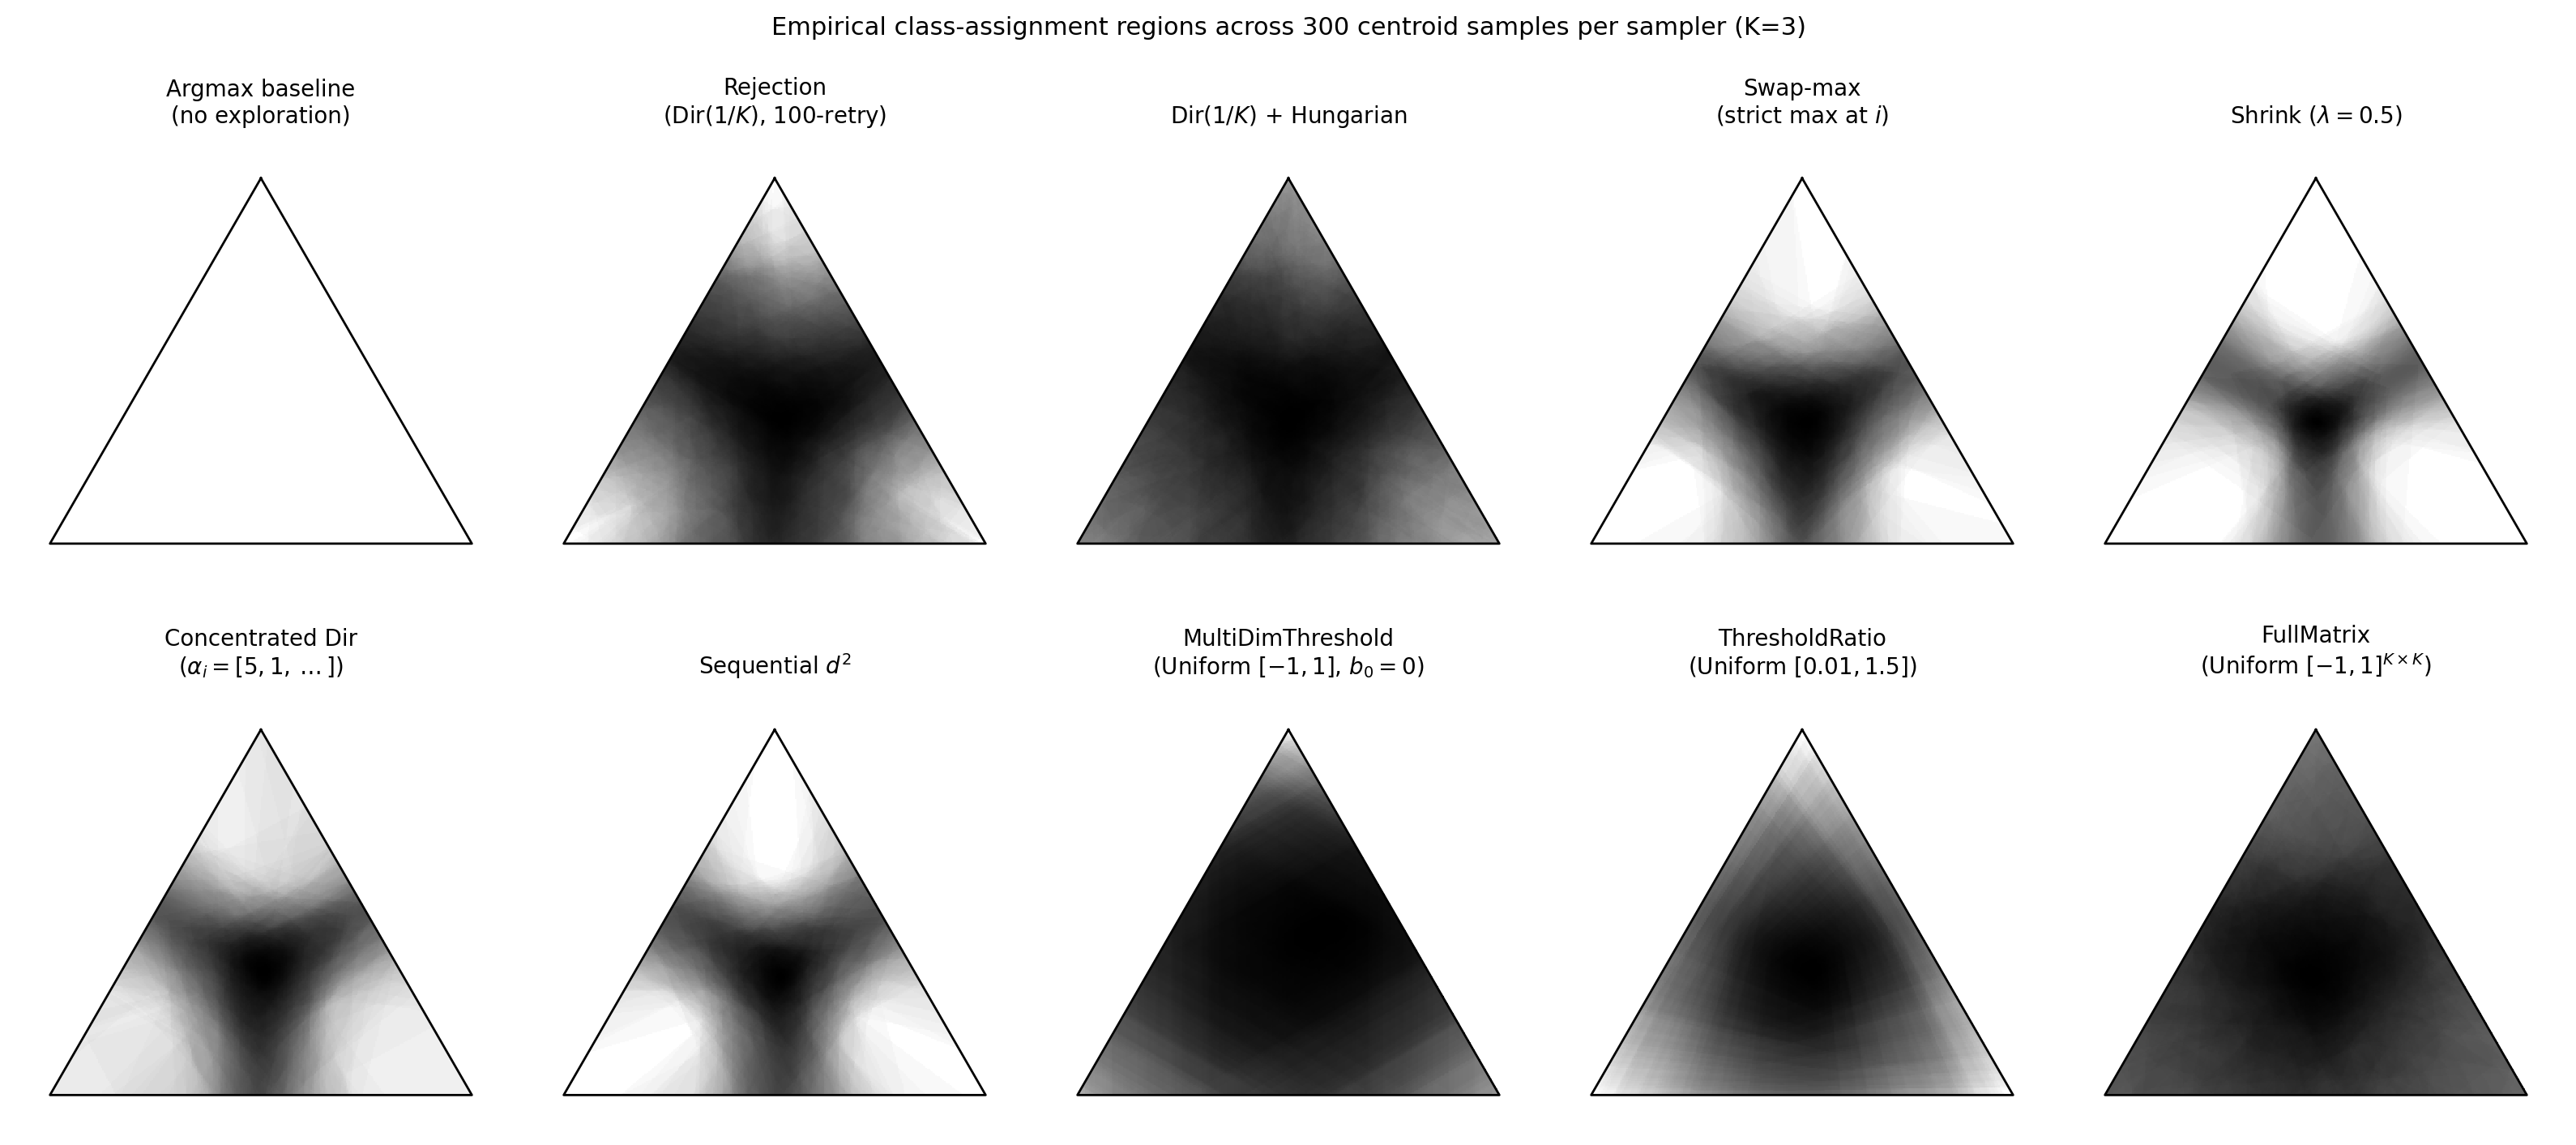
\includegraphics[width=\textwidth]{figures/sampler_partition_overlay.png}
    \caption{Classification disagreement across $300$ sampled configurations per panel at $K=3$. Shade at each grid point is $1 - H(\mathbf{f})$, where $\mathbf{f}$ is the empirical class-fraction vector across samples and $H$ is the Shannon entropy normalised to $[0, 1]$: white marks unanimous agreement on a single class and black marks the uniform distribution over three classes. Rejection and Dir$(1/K)$+Hungarian exhibit dark vertex regions, indicating that the pure-class corners are not consistently decoded to their own class; Shrink keeps the vertex regions white and the interior near-white, reflecting its limited exploration range; Sequential $d^2$ keeps the vertex regions white while producing interior disagreement comparable to Hungarian.}\label{fig:sampler_partition_overlay}
\end{figure}

The rejection baseline and sequential $d^2$ are the two retry-based samplers; Figure~\ref{fig:sampler_rejection_rate} reports their exhaustion rate as a function of $K$ for $M \in \{10, 100, 500\}$. The rejection baseline asymptotes at one for every $M$, confirming that its failure mode is structural in $K$ rather than budget-bounded. Sequential $d^2$ exhausts at zero for $M \geq 100$ across the entire sweep, because the joint acceptance condition~\eqref{eq:seqd2_accept} concentrates the sampler on configurations satisfying the invariant rather than filtering from an uninformative prior.

\begin{figure}[H]
    \centering
    % Auto-generated by experiments.analysis.generate_sampler_overlay_figure --- do not edit.
\resizebox{\textwidth}{!}{%
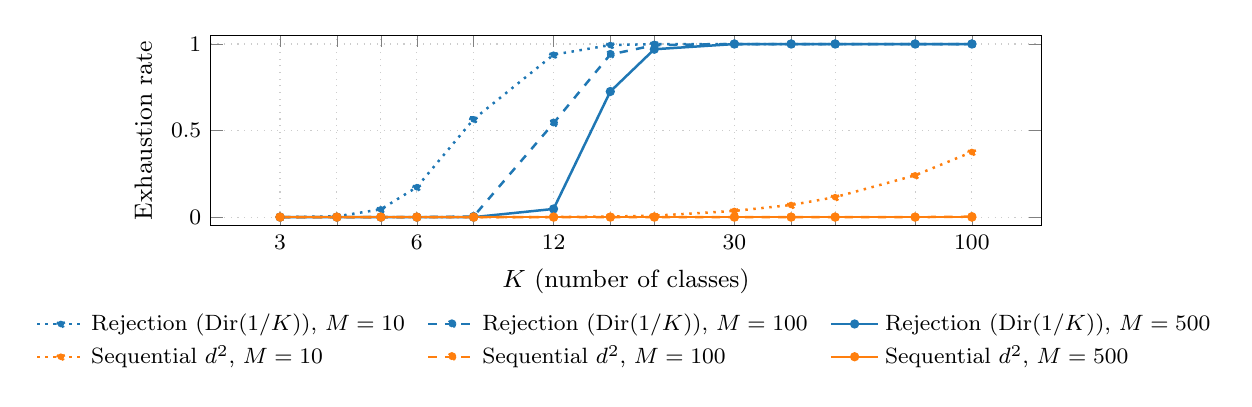
\begin{tikzpicture}
\begin{axis}[
    width=\textwidth, height=4.0cm,
    xlabel={$K$ (number of classes)},
    ylabel={Exhaustion rate},
    xmode=log, log basis x=10, log ticks with fixed point,
    xtick={3,4,5,6,8,12,16,20,30,40,50,75,100},
    xticklabels={3,,,6,,12,,,30,,,,100},
    ymin=-0.05, ymax=1.05,
    grid=major, grid style={dotted, gray!40},
    legend cell align=left,
    legend style={
        at={(0.5,-0.40)}, anchor=north,
        legend columns=3,
        /tikz/every even column/.append style={column sep=0.6em},
        font=\footnotesize, draw=none, fill=none,
    },
    tick label style={font=\footnotesize},
    label style={font=\small},
]
\addplot[
    color={rgb,255:red,31; green,119; blue,180}, mark=*, mark size=1.2pt, line width=0.9pt, dotted,
    error bars/y dir=both, error bars/y explicit,
    error bars/error bar style={line width=0.5pt}
] coordinates {
        (3, 0) +- (0, 0)
        (4, 0.00466667) +- (0, 0.00152853)
        (5, 0.045) +- (0, 0.00629695)
        (6, 0.173) +- (0, 0.0107969)
        (8, 0.565167) +- (0, 0.0141756)
        (12, 0.938333) +- (0, 0.00661025)
        (16, 0.994) +- (0, 0.00187206)
        (20, 0.9995) +- (0, 0.000535196)
        (30, 1) +- (0, 0)
        (40, 1) +- (0, 0)
        (50, 1) +- (0, 0)
        (75, 1) +- (0, 0)
        (100, 1) +- (0, 0)
    };
\addlegendentry{Rejection (Dir$(1/K)$), $M=10$}
\addplot[
    color={rgb,255:red,31; green,119; blue,180}, mark=*, mark size=1.2pt, line width=0.9pt, dashed,
    error bars/y dir=both, error bars/y explicit,
    error bars/error bar style={line width=0.5pt}
] coordinates {
        (3, 0) +- (0, 0)
        (4, 0) +- (0, 0)
        (5, 0) +- (0, 0)
        (6, 0) +- (0, 0)
        (8, 0.00366667) +- (0, 0.00221809)
        (12, 0.542833) +- (0, 0.00978595)
        (16, 0.9395) +- (0, 0.00650361)
        (20, 0.993167) +- (0, 0.00234487)
        (30, 1) +- (0, 0)
        (40, 1) +- (0, 0)
        (50, 1) +- (0, 0)
        (75, 1) +- (0, 0)
        (100, 1) +- (0, 0)
    };
\addlegendentry{Rejection (Dir$(1/K)$), $M=100$}
\addplot[
    color={rgb,255:red,31; green,119; blue,180}, mark=*, mark size=1.2pt, line width=0.9pt, solid,
    error bars/y dir=both, error bars/y explicit,
    error bars/error bar style={line width=0.5pt}
] coordinates {
        (3, 0) +- (0, 0)
        (4, 0) +- (0, 0)
        (5, 0) +- (0, 0)
        (6, 0) +- (0, 0)
        (8, 0) +- (0, 0)
        (12, 0.0473333) +- (0, 0.00520513)
        (16, 0.725667) +- (0, 0.0132638)
        (20, 0.969833) +- (0, 0.00427829)
        (30, 0.999833) +- (0, 0.000326667)
        (40, 1) +- (0, 0)
        (50, 1) +- (0, 0)
        (75, 1) +- (0, 0)
        (100, 1) +- (0, 0)
    };
\addlegendentry{Rejection (Dir$(1/K)$), $M=500$}
\addplot[
    color={rgb,255:red,255; green,127; blue,14}, mark=*, mark size=1.2pt, line width=0.9pt, dotted,
    error bars/y dir=both, error bars/y explicit,
    error bars/error bar style={line width=0.5pt}
] coordinates {
        (3, 0) +- (0, 0)
        (4, 0) +- (0, 0)
        (5, 0) +- (0, 0)
        (6, 0) +- (0, 0)
        (8, 0) +- (0, 0)
        (12, 0.000833333) +- (0, 0.000803668)
        (16, 0.0035) +- (0, 0.00153403)
        (20, 0.00833333) +- (0, 0.00160734)
        (30, 0.0358333) +- (0, 0.0049)
        (40, 0.0701667) +- (0, 0.00537239)
        (50, 0.115333) +- (0, 0.00455611)
        (75, 0.241333) +- (0, 0.0132832)
        (100, 0.376333) +- (0, 0.0108385)
    };
\addlegendentry{Sequential $d^2$, $M=10$}
\addplot[
    color={rgb,255:red,255; green,127; blue,14}, mark=*, mark size=1.2pt, line width=0.9pt, dashed,
    error bars/y dir=both, error bars/y explicit,
    error bars/error bar style={line width=0.5pt}
] coordinates {
        (3, 0) +- (0, 0)
        (4, 0) +- (0, 0)
        (5, 0) +- (0, 0)
        (6, 0) +- (0, 0)
        (8, 0) +- (0, 0)
        (12, 0) +- (0, 0)
        (16, 0) +- (0, 0)
        (20, 0) +- (0, 0)
        (30, 0) +- (0, 0)
        (40, 0.000166667) +- (0, 0.000326667)
        (50, 0.000333333) +- (0, 0.000449655)
        (75, 0.000166667) +- (0, 0.000326667)
        (100, 0.00266667) +- (0, 0.00154316)
    };
\addlegendentry{Sequential $d^2$, $M=100$}
\addplot[
    color={rgb,255:red,255; green,127; blue,14}, mark=*, mark size=1.2pt, line width=0.9pt, solid,
    error bars/y dir=both, error bars/y explicit,
    error bars/error bar style={line width=0.5pt}
] coordinates {
        (3, 0) +- (0, 0)
        (4, 0) +- (0, 0)
        (5, 0) +- (0, 0)
        (6, 0) +- (0, 0)
        (8, 0) +- (0, 0)
        (12, 0) +- (0, 0)
        (16, 0) +- (0, 0)
        (20, 0) +- (0, 0)
        (30, 0) +- (0, 0)
        (40, 0) +- (0, 0)
        (50, 0) +- (0, 0)
        (75, 0) +- (0, 0)
        (100, 0) +- (0, 0)
    };
\addlegendentry{Sequential $d^2$, $M=500$}
\end{axis}
\end{tikzpicture}%
}

    \caption{Exhaustion rate versus $K$ for the two retry-based samplers under three retry budgets $M \in \{10, 100, 500\}$. Colour identifies the sampler (blue: rejection baseline, orange: sequential $d^2$); line style identifies the budget (dotted: $M{=}10$, dashed: $M{=}100$, solid: $M{=}500$). Each marker is the fraction of sampler calls (over $20$ trials of $300$ draws each) that exhausted the budget without producing a valid configuration; error bars are $95\%$ confidence intervals across trials.}\label{fig:sampler_rejection_rate}
\end{figure}

Figure~\ref{fig:sampler_metrics_vs_k} sweeps $K \in \{3, 4, 5, 6, 8, 12, 16, 20, 30, 40, 50, 75, 100\}$ and reports three summary statistics per sampler, averaged over only those draws that did not raise. The left panel is the fraction of successful draws satisfying~\eqref{eq:dlc}; sequential $d^2$, Shrink, argmax, and ThresholdRatio remain at $1.0$ by construction, while Hungarian, Swap-max, Concentrated Dirichlet, MultidimensionalThreshold, and FullMatrix decrease monotonically with $K$. The middle panel is the mean disagreement entropy across a simplex grid (the average greyscale darkness in Figure~\ref{fig:sampler_partition_overlay}), measuring how much independent draws of the same sampler disagree on the same input. The right panel is the partition deviation from argmax: the fraction of grid points whose predicted class differs from $\arg\max_{j \in \mathcal{Y}} p_j$, averaged over successful draws. The two panels separate exploration magnitude (deviation) from exploration variability (entropy): a sampler that consistently produces a partition far from argmax scores high on the right and low in the middle.

\begin{figure}[H]
    \centering
    % Auto-generated by experiments.analysis.generate_sampler_overlay_figure --- do not edit.
\begin{tikzpicture}
\begin{groupplot}[
    group style={group size=3 by 1, horizontal sep=0.9cm},
    width=0.34\textwidth, height=5.2cm,
    xmode=log, log basis x=10, log ticks with fixed point,
    xtick={3,4,5,6,8,12,16,20,30,40,50,75,100},
    xticklabels={3,,,6,,12,,,30,,,,100},
    ymin=0, ymax=1.05,
    xlabel={$K$ (number of classes)},
    grid=major, grid style={dotted, gray!40},
    tick label style={font=\footnotesize},
    label style={font=\small},
    title style={font=\small, align=center},
]
\nextgroupplot[title={Pure-class vertex $\to$ own class}]
\addplot[
    color={rgb,255:red,255; green,127; blue,14}, mark=*, mark size=1.2pt, line width=0.9pt, solid,
    error bars/y dir=both, error bars/y explicit,
    error bars/error bar style={line width=0.5pt}
] coordinates {
        (3, 0.6535) +- (0, 0.0131051)
        (4, 0.4095) +- (0, 0.0118899)
        (5, 0.263333) +- (0, 0.00895555)
        (6, 0.165) +- (0, 0.00993659)
        (8, 0.0596667) +- (0, 0.00415644)
        (12, 0.006) +- (0, 0.00161431)
        (16, 0.000666667) +- (0, 0.000764266)
        (20, 0) +- (0, 0)
        (30, 0) +- (0, 0)
        (40, 0) +- (0, 0)
        (50, 0) +- (0, 0)
        (75, 0) +- (0, 0)
        (100, 0) +- (0, 0)
    };
\addplot[
    color={rgb,255:red,44; green,160; blue,44}, mark=*, mark size=1.2pt, line width=0.9pt, solid,
    error bars/y dir=both, error bars/y explicit,
    error bars/error bar style={line width=0.5pt}
] coordinates {
        (3, 0.9985) +- (0, 0.00110905)
        (4, 0.995667) +- (0, 0.00117064)
        (5, 0.990167) +- (0, 0.0023923)
        (6, 0.988333) +- (0, 0.00266019)
        (8, 0.981333) +- (0, 0.00269793)
        (12, 0.959833) +- (0, 0.0045084)
        (16, 0.939167) +- (0, 0.00603042)
        (20, 0.915833) +- (0, 0.00896652)
        (30, 0.8755) +- (0, 0.00752827)
        (40, 0.828833) +- (0, 0.0093155)
        (50, 0.789) +- (0, 0.00865058)
        (75, 0.687833) +- (0, 0.00967048)
        (100, 0.613667) +- (0, 0.0129882)
    };
\addplot[
    color={rgb,255:red,148; green,103; blue,189}, mark=*, mark size=1.2pt, line width=0.9pt, solid,
    error bars/y dir=both, error bars/y explicit,
    error bars/error bar style={line width=0.5pt}
] coordinates {
        (3, 0.973333) +- (0, 0.00328381)
        (4, 0.924667) +- (0, 0.00551528)
        (5, 0.858333) +- (0, 0.00692559)
        (6, 0.771) +- (0, 0.0113666)
        (8, 0.576667) +- (0, 0.00970208)
        (12, 0.2375) +- (0, 0.0101311)
        (16, 0.0646667) +- (0, 0.00739466)
        (20, 0.0125) +- (0, 0.00295524)
        (30, 0) +- (0, 0)
        (40, 0) +- (0, 0)
        (50, 0) +- (0, 0)
        (75, 0) +- (0, 0)
        (100, 0) +- (0, 0)
    };
\addplot[
    color={rgb,255:red,227; green,119; blue,194}, mark=*, mark size=1.2pt, line width=0.9pt, solid,
    error bars/y dir=both, error bars/y explicit,
    error bars/error bar style={line width=0.5pt}
] coordinates {
        (3, 0.749333) +- (0, 0.0097782)
        (4, 0.5015) +- (0, 0.0120978)
        (5, 0.313333) +- (0, 0.0140124)
        (6, 0.191333) +- (0, 0.0103453)
        (8, 0.0585) +- (0, 0.00705376)
        (12, 0.00616667) +- (0, 0.00228667)
        (16, 0) +- (0, 0)
        (20, 0) +- (0, 0)
        (30, 0) +- (0, 0)
        (40, 0) +- (0, 0)
        (50, 0) +- (0, 0)
        (75, 0) +- (0, 0)
        (100, 0) +- (0, 0)
    };
\addplot[
    color={rgb,255:red,188; green,189; blue,34}, mark=*, mark size=1.2pt, line width=0.9pt, solid,
    error bars/y dir=both, error bars/y explicit,
    error bars/error bar style={line width=0.5pt}
] coordinates {
        (3, 0.496667) +- (0, 0.00912946)
        (4, 0.2805) +- (0, 0.0110679)
        (5, 0.159167) +- (0, 0.00952536)
        (6, 0.083) +- (0, 0.00560618)
        (8, 0.0233333) +- (0, 0.00373211)
        (12, 0.00133333) +- (0, 0.000873972)
        (16, 0.000333333) +- (0, 0.000653333)
        (20, 0) +- (0, 0)
        (30, 0) +- (0, 0)
        (40, 0) +- (0, 0)
        (50, 0) +- (0, 0)
        (75, 0) +- (0, 0)
        (100, 0) +- (0, 0)
    };
\nextgroupplot[title={Mean disagreement entropy \\ (simplex grid)}]
\addplot[
    color={rgb,255:red,31; green,119; blue,180}, mark=*, mark size=1.2pt, line width=0.9pt, solid,
    error bars/y dir=both, error bars/y explicit,
    error bars/error bar style={line width=0.5pt}
] coordinates {
        (3, 0) +- (0, 0)
        (4, 0) +- (0, 0)
        (5, 0) +- (0, 0)
        (6, 0) +- (0, 0)
        (8, 0) +- (0, 0)
        (12, 0) +- (0, 0)
        (16, 0) +- (0, 0)
        (20, 0) +- (0, 0)
        (30, 0) +- (0, 0)
        (40, 0) +- (0, 0)
        (50, 0) +- (0, 0)
        (75, 0) +- (0, 0)
        (100, 0) +- (0, 0)
    };
\addplot[
    color={rgb,255:red,255; green,127; blue,14}, mark=*, mark size=1.2pt, line width=0.9pt, solid,
    error bars/y dir=both, error bars/y explicit,
    error bars/error bar style={line width=0.5pt}
] coordinates {
        (3, 0.77837) +- (0, 0.00585969)
        (4, 0.813056) +- (0, 0.00472878)
        (5, 0.832734) +- (0, 0.00288057)
        (6, 0.850708) +- (0, 0.00320886)
        (8, 0.875537) +- (0, 0.00223782)
        (12, 0.911993) +- (0, 0.00151792)
        (16, 0.930978) +- (0, 0.00146938)
        (20, 0.943361) +- (0, 0.00129199)
        (30, 0.960389) +- (0, 0.00107288)
        (40, 0.965026) +- (0, 0.000798964)
        (50, 0.967955) +- (0, 0.000908311)
        (75, 0.964269) +- (0, 0.00131859)
        (100, 0.958256) +- (0, 0.00152893)
    };
\addplot[
    color={rgb,255:red,44; green,160; blue,44}, mark=*, mark size=1.2pt, line width=0.9pt, solid,
    error bars/y dir=both, error bars/y explicit,
    error bars/error bar style={line width=0.5pt}
] coordinates {
        (3, 0.372799) +- (0, 0.00593744)
        (4, 0.447166) +- (0, 0.0058969)
        (5, 0.505565) +- (0, 0.00515114)
        (6, 0.557794) +- (0, 0.00371621)
        (8, 0.642779) +- (0, 0.00429098)
        (12, 0.759441) +- (0, 0.00267977)
        (16, 0.825428) +- (0, 0.00347969)
        (20, 0.865639) +- (0, 0.00256653)
        (30, 0.917364) +- (0, 0.0017437)
        (40, 0.940013) +- (0, 0.00130232)
        (50, 0.950407) +- (0, 0.000909989)
        (75, 0.958581) +- (0, 0.00100233)
        (100, 0.953611) +- (0, 0.00225912)
    };
\addplot[
    color={rgb,255:red,214; green,39; blue,40}, mark=*, mark size=1.2pt, line width=0.9pt, solid,
    error bars/y dir=both, error bars/y explicit,
    error bars/error bar style={line width=0.5pt}
] coordinates {
        (3, 0.265537) +- (0, 0.00562947)
        (4, 0.249357) +- (0, 0.00395823)
        (5, 0.234437) +- (0, 0.00394318)
        (6, 0.219159) +- (0, 0.00247256)
        (8, 0.200843) +- (0, 0.00204682)
        (12, 0.176409) +- (0, 0.0024103)
        (16, 0.162717) +- (0, 0.00180198)
        (20, 0.152623) +- (0, 0.0018185)
        (30, 0.136546) +- (0, 0.00158247)
        (40, 0.126753) +- (0, 0.0012205)
        (50, 0.119318) +- (0, 0.00128798)
        (75, 0.109573) +- (0, 0.00092299)
        (100, 0.103191) +- (0, 0.00129697)
    };
\addplot[
    color={rgb,255:red,148; green,103; blue,189}, mark=*, mark size=1.2pt, line width=0.9pt, solid,
    error bars/y dir=both, error bars/y explicit,
    error bars/error bar style={line width=0.5pt}
] coordinates {
        (3, 0.371256) +- (0, 0.00625153)
        (4, 0.439725) +- (0, 0.00531927)
        (5, 0.492492) +- (0, 0.00617642)
        (6, 0.52919) +- (0, 0.00539672)
        (8, 0.591514) +- (0, 0.0035765)
        (12, 0.667666) +- (0, 0.00294207)
        (16, 0.716458) +- (0, 0.00339461)
        (20, 0.750384) +- (0, 0.00194903)
        (30, 0.802315) +- (0, 0.00150149)
        (40, 0.833899) +- (0, 0.000708931)
        (50, 0.852921) +- (0, 0.00119884)
        (75, 0.879233) +- (0, 0.000730223)
        (100, 0.890571) +- (0, 0.000618399)
    };
\addplot[
    color={rgb,255:red,140; green,86; blue,75}, mark=*, mark size=1.2pt, line width=0.9pt, solid,
    error bars/y dir=both, error bars/y explicit,
    error bars/error bar style={line width=0.5pt}
] coordinates {
        (3, 0.346799) +- (0, 0.00527885)
        (4, 0.402057) +- (0, 0.00569766)
        (5, 0.442914) +- (0, 0.00517294)
        (6, 0.469562) +- (0, 0.00338183)
        (8, 0.519007) +- (0, 0.0024014)
        (12, 0.582268) +- (0, 0.00253397)
        (16, 0.623343) +- (0, 0.00242087)
        (20, 0.653314) +- (0, 0.00204929)
        (30, 0.702519) +- (0, 0.00170069)
        (40, 0.733939) +- (0, 0.000966374)
        (50, 0.754689) +- (0, 0.00146493)
        (75, 0.788332) +- (0, 0.00110195)
        (100, 0.806591) +- (0, 0.00073574)
    };
\addplot[
    color={rgb,255:red,227; green,119; blue,194}, mark=*, mark size=1.2pt, line width=0.9pt, solid,
    error bars/y dir=both, error bars/y explicit,
    error bars/error bar style={line width=0.5pt}
] coordinates {
        (3, 0.841806) +- (0, 0.00380629)
        (4, 0.87784) +- (0, 0.00364437)
        (5, 0.891622) +- (0, 0.00362347)
        (6, 0.897392) +- (0, 0.00364769)
        (8, 0.908875) +- (0, 0.00318785)
        (12, 0.92922) +- (0, 0.00180897)
        (16, 0.939459) +- (0, 0.00157958)
        (20, 0.946445) +- (0, 0.0017324)
        (30, 0.95289) +- (0, 0.00122959)
        (40, 0.954904) +- (0, 0.000964237)
        (50, 0.952766) +- (0, 0.00135665)
        (75, 0.949451) +- (0, 0.00177961)
        (100, 0.940819) +- (0, 0.00245238)
    };
\addplot[
    color={rgb,255:red,127; green,127; blue,127}, mark=*, mark size=1.2pt, line width=0.9pt, solid,
    error bars/y dir=both, error bars/y explicit,
    error bars/error bar style={line width=0.5pt}
] coordinates {
        (3, 0.647221) +- (0, 0.0075065)
        (4, 0.682117) +- (0, 0.00784401)
        (5, 0.708197) +- (0, 0.00661577)
        (6, 0.724471) +- (0, 0.00531476)
        (8, 0.754369) +- (0, 0.00480233)
        (12, 0.782009) +- (0, 0.0032986)
        (16, 0.795448) +- (0, 0.00299954)
        (20, 0.803172) +- (0, 0.00265332)
        (30, 0.815186) +- (0, 0.00308205)
        (40, 0.817452) +- (0, 0.00249688)
        (50, 0.818564) +- (0, 0.00210879)
        (75, 0.814271) +- (0, 0.00161582)
        (100, 0.80669) +- (0, 0.00105788)
    };
\addplot[
    color={rgb,255:red,188; green,189; blue,34}, mark=*, mark size=1.2pt, line width=0.9pt, solid,
    error bars/y dir=both, error bars/y explicit,
    error bars/error bar style={line width=0.5pt}
] coordinates {
        (3, 0.819566) +- (0, 0.00501197)
        (4, 0.839068) +- (0, 0.0056958)
        (5, 0.851929) +- (0, 0.00361308)
        (6, 0.862499) +- (0, 0.00290218)
        (8, 0.876193) +- (0, 0.00210679)
        (12, 0.900123) +- (0, 0.00108741)
        (16, 0.914479) +- (0, 0.000905028)
        (20, 0.924322) +- (0, 0.000887098)
        (30, 0.93831) +- (0, 0.000581018)
        (40, 0.945657) +- (0, 0.000512726)
        (50, 0.948428) +- (0, 0.000379355)
        (75, 0.949459) +- (0, 0.000388088)
        (100, 0.945453) +- (0, 0.000252369)
    };
\nextgroupplot[title={Partition deviation \\ from argmax},
    legend to name=samplerlegendmetrics,
    legend style={
        font=\footnotesize, draw=none, fill=none,
        legend columns=4,
        /tikz/every even column/.append style={column sep=0.6em},
    },
    legend cell align=left]
\addplot[
    color={rgb,255:red,31; green,119; blue,180}, mark=*, mark size=1.2pt, line width=0.9pt, solid,
    error bars/y dir=both, error bars/y explicit,
    error bars/error bar style={line width=0.5pt}
] coordinates {
        (3, 0) +- (0, 0)
        (4, 0) +- (0, 0)
        (5, 0) +- (0, 0)
        (6, 0) +- (0, 0)
        (8, 0) +- (0, 0)
        (12, 0) +- (0, 0)
        (16, 0) +- (0, 0)
        (20, 0) +- (0, 0)
        (30, 0) +- (0, 0)
        (40, 0) +- (0, 0)
        (50, 0) +- (0, 0)
        (75, 0) +- (0, 0)
        (100, 0) +- (0, 0)
    };
\addplot[
    color={rgb,255:red,255; green,127; blue,14}, mark=*, mark size=1.2pt, line width=0.9pt, solid,
    error bars/y dir=both, error bars/y explicit,
    error bars/error bar style={line width=0.5pt}
] coordinates {
        (3, 0.367732) +- (0, 0.0043432)
        (4, 0.459895) +- (0, 0.00434397)
        (5, 0.522282) +- (0, 0.00288499)
        (6, 0.572665) +- (0, 0.00350981)
        (8, 0.647334) +- (0, 0.00269877)
        (12, 0.747536) +- (0, 0.00188312)
        (16, 0.805781) +- (0, 0.00187474)
        (20, 0.84587) +- (0, 0.00156137)
        (30, 0.904187) +- (0, 0.000748952)
        (40, 0.933224) +- (0, 0.000728659)
        (50, 0.950068) +- (0, 0.000569008)
        (75, 0.971754) +- (0, 0.00043202)
        (100, 0.980786) +- (0, 0.000229619)
    };
\addplot[
    color={rgb,255:red,44; green,160; blue,44}, mark=*, mark size=1.2pt, line width=0.9pt, solid,
    error bars/y dir=both, error bars/y explicit,
    error bars/error bar style={line width=0.5pt}
] coordinates {
        (3, 0.168111) +- (0, 0.00338015)
        (4, 0.241462) +- (0, 0.00362543)
        (5, 0.30383) +- (0, 0.00350984)
        (6, 0.359529) +- (0, 0.00300043)
        (8, 0.458015) +- (0, 0.00336196)
        (12, 0.603403) +- (0, 0.00249757)
        (16, 0.697615) +- (0, 0.00320266)
        (20, 0.761199) +- (0, 0.00256102)
        (30, 0.85422) +- (0, 0.00145083)
        (40, 0.900721) +- (0, 0.00115666)
        (50, 0.927489) +- (0, 0.00105105)
        (75, 0.960694) +- (0, 0.000699423)
        (100, 0.974178) +- (0, 0.000359782)
    };
\addplot[
    color={rgb,255:red,214; green,39; blue,40}, mark=*, mark size=1.2pt, line width=0.9pt, solid,
    error bars/y dir=both, error bars/y explicit,
    error bars/error bar style={line width=0.5pt}
] coordinates {
        (3, 0.124882) +- (0, 0.00261134)
        (4, 0.144149) +- (0, 0.00246368)
        (5, 0.154808) +- (0, 0.00286235)
        (6, 0.159126) +- (0, 0.00213982)
        (8, 0.168398) +- (0, 0.00231317)
        (12, 0.174299) +- (0, 0.00289588)
        (16, 0.178388) +- (0, 0.00243734)
        (20, 0.179814) +- (0, 0.0026394)
        (30, 0.182278) +- (0, 0.00290332)
        (40, 0.182722) +- (0, 0.00223039)
        (50, 0.182901) +- (0, 0.00257952)
        (75, 0.185486) +- (0, 0.00150741)
        (100, 0.185081) +- (0, 0.00256207)
    };
\addplot[
    color={rgb,255:red,148; green,103; blue,189}, mark=*, mark size=1.2pt, line width=0.9pt, solid,
    error bars/y dir=both, error bars/y explicit,
    error bars/error bar style={line width=0.5pt}
] coordinates {
        (3, 0.157405) +- (0, 0.00303679)
        (4, 0.225645) +- (0, 0.0033817)
        (5, 0.283244) +- (0, 0.00409966)
        (6, 0.328151) +- (0, 0.00355737)
        (8, 0.406721) +- (0, 0.00267064)
        (12, 0.514332) +- (0, 0.00288974)
        (16, 0.587824) +- (0, 0.00310824)
        (20, 0.641093) +- (0, 0.00205485)
        (30, 0.728017) +- (0, 0.00168531)
        (40, 0.782648) +- (0, 0.000894158)
        (50, 0.818767) +- (0, 0.00140421)
        (75, 0.874868) +- (0, 0.000998815)
        (100, 0.905719) +- (0, 0.000880204)
    };
\addplot[
    color={rgb,255:red,140; green,86; blue,75}, mark=*, mark size=1.2pt, line width=0.9pt, solid,
    error bars/y dir=both, error bars/y explicit,
    error bars/error bar style={line width=0.5pt}
] coordinates {
        (3, 0.159691) +- (0, 0.00284143)
        (4, 0.220365) +- (0, 0.00332963)
        (5, 0.270407) +- (0, 0.00367207)
        (6, 0.307172) +- (0, 0.0027213)
        (8, 0.374889) +- (0, 0.00201705)
        (12, 0.46779) +- (0, 0.0024261)
        (16, 0.531006) +- (0, 0.00238303)
        (20, 0.579214) +- (0, 0.00235585)
        (30, 0.659605) +- (0, 0.00190598)
        (40, 0.711961) +- (0, 0.00126868)
        (50, 0.748901) +- (0, 0.00185437)
        (75, 0.80954) +- (0, 0.00137474)
        (100, 0.846412) +- (0, 0.00126185)
    };
\addplot[
    color={rgb,255:red,227; green,119; blue,194}, mark=*, mark size=1.2pt, line width=0.9pt, solid,
    error bars/y dir=both, error bars/y explicit,
    error bars/error bar style={line width=0.5pt}
] coordinates {
        (3, 0.444159) +- (0, 0.00374994)
        (4, 0.568977) +- (0, 0.00395233)
        (5, 0.64859) +- (0, 0.00420293)
        (6, 0.699492) +- (0, 0.00383452)
        (8, 0.766746) +- (0, 0.00246998)
        (12, 0.832669) +- (0, 0.00245901)
        (16, 0.865284) +- (0, 0.00168187)
        (20, 0.887737) +- (0, 0.0011488)
        (30, 0.919201) +- (0, 0.000942476)
        (40, 0.936399) +- (0, 0.00060299)
        (50, 0.946984) +- (0, 0.000466637)
        (75, 0.962395) +- (0, 0.000427416)
        (100, 0.970486) +- (0, 0.000354685)
    };
\addplot[
    color={rgb,255:red,127; green,127; blue,127}, mark=*, mark size=1.2pt, line width=0.9pt, solid,
    error bars/y dir=both, error bars/y explicit,
    error bars/error bar style={line width=0.5pt}
] coordinates {
        (3, 0.311681) +- (0, 0.00548634)
        (4, 0.399075) +- (0, 0.00606963)
        (5, 0.465765) +- (0, 0.00605427)
        (6, 0.51548) +- (0, 0.00487938)
        (8, 0.595761) +- (0, 0.00409933)
        (12, 0.688682) +- (0, 0.00325143)
        (16, 0.742075) +- (0, 0.00232123)
        (20, 0.779371) +- (0, 0.00210046)
        (30, 0.835683) +- (0, 0.00189765)
        (40, 0.864892) +- (0, 0.0014669)
        (50, 0.884106) +- (0, 0.00128854)
        (75, 0.911753) +- (0, 0.000918897)
        (100, 0.926173) +- (0, 0.000655623)
    };
\addplot[
    color={rgb,255:red,188; green,189; blue,34}, mark=*, mark size=1.2pt, line width=0.9pt, solid,
    error bars/y dir=both, error bars/y explicit,
    error bars/error bar style={line width=0.5pt}
] coordinates {
        (3, 0.403405) +- (0, 0.00445641)
        (4, 0.490825) +- (0, 0.00499481)
        (5, 0.552072) +- (0, 0.00343839)
        (6, 0.59841) +- (0, 0.00299632)
        (8, 0.662986) +- (0, 0.00232583)
        (12, 0.747383) +- (0, 0.00135307)
        (16, 0.797368) +- (0, 0.000940028)
        (20, 0.831009) +- (0, 0.000968433)
        (30, 0.8819) +- (0, 0.000462139)
        (40, 0.910841) +- (0, 0.000558771)
        (50, 0.928291) +- (0, 0.000424632)
        (75, 0.953425) +- (0, 0.000316544)
        (100, 0.96624) +- (0, 0.000197039)
    };
\addlegendimage{color={rgb,255:red,31; green,119; blue,180}, mark=*, mark size=1.2pt, line width=0.9pt}
\addlegendentry{Argmax}
\addlegendimage{color={rgb,255:red,255; green,127; blue,14}, mark=*, mark size=1.2pt, line width=0.9pt}
\addlegendentry{Hungarian (Dir$(1/K)$)}
\addlegendimage{color={rgb,255:red,44; green,160; blue,44}, mark=*, mark size=1.2pt, line width=0.9pt}
\addlegendentry{Swap-max}
\addlegendimage{color={rgb,255:red,214; green,39; blue,40}, mark=*, mark size=1.2pt, line width=0.9pt}
\addlegendentry{Shrink ($\lambda=0.5$)}
\addlegendimage{color={rgb,255:red,148; green,103; blue,189}, mark=*, mark size=1.2pt, line width=0.9pt}
\addlegendentry{Concentrated Dir}
\addlegendimage{color={rgb,255:red,140; green,86; blue,75}, mark=*, mark size=1.2pt, line width=0.9pt}
\addlegendentry{Sequential $d^2$}
\addlegendimage{color={rgb,255:red,227; green,119; blue,194}, mark=*, mark size=1.2pt, line width=0.9pt}
\addlegendentry{MultiDimThreshold}
\addlegendimage{color={rgb,255:red,127; green,127; blue,127}, mark=*, mark size=1.2pt, line width=0.9pt}
\addlegendentry{ThresholdRatio}
\addlegendimage{color={rgb,255:red,188; green,189; blue,34}, mark=*, mark size=1.2pt, line width=0.9pt}
\addlegendentry{FullMatrix}
\end{groupplot}
\end{tikzpicture}%
\par\smallskip
\centerline{\ref{samplerlegendmetrics}}

    \caption{Sampler metrics as a function of $K$. Markers denote the mean over $20$ independent trials of $300$ sampled configurations; error bars are $95\%$ confidence intervals across trials. All metrics are averaged only over draws that did not raise during construction. Left: fraction of successful draws satisfying $\arg\min_{j \in \mathcal{Y}}\|\mathbf{e}_k-\boldsymbol{\mu}_j\|_2 = \{k\}$ for every $k$. Middle: mean over a simplex grid of the normalised Shannon entropy of the empirical class-fraction vector across samples (the grid-average of the greyscale darkness in Figure~\ref{fig:sampler_partition_overlay}). Right: mean over successful draws of the fraction of grid points classified differently from $\arg\max_{j \in \mathcal{Y}} p_j$.}\label{fig:sampler_metrics_vs_k}
\end{figure}

Among the six Voronoi samplers compared, sequential $d^2$ is the only one that satisfies~\eqref{eq:dlc} with probability one across the entire sweep while producing a partition-deviation footprint comparable to Hungarian; it is therefore the sampler we adopt for the Voronoi optimizer. Shrink also satisfies~\eqref{eq:dlc}, but its reachable configurations stay near the argmax tessellation, so its partition-deviation footprint is small.

Swap-max and Concentrated Dirichlet enforce only a per-centroid marginal of~\eqref{eq:dlc}, not the joint condition across centroids, which is why the left panel of Figure~\ref{fig:sampler_metrics_vs_k} shows their satisfaction fraction decaying as $K$ grows. For swap-max the decay is exact: applying~\eqref{eq:dsq_identity} to~\eqref{eq:dlc}, the constraint is equivalent to
\begin{equation}
    \|\boldsymbol{\mu}_k\|_2^2 - 2\,\boldsymbol{\mu}_k[k] \;<\; \|\boldsymbol{\mu}_j\|_2^2 - 2\,\boldsymbol{\mu}_j[k] \qquad \text{for all } j \neq k,
    \label{eq:voronoi_invariant_expanded}
\end{equation}
which involves the off-diagonal entries $\boldsymbol{\mu}_j[k]$ and the squared norms $\|\boldsymbol{\mu}_j\|_2^2$ that swap-max leaves uncontrolled, so it cannot hold~\eqref{eq:voronoi_invariant_expanded} as $K$ grows, consistent with the observed decay; Concentrated Dirichlet's per-centroid marginal bias breaks~\eqref{eq:dlc} for the same reason.

A broader observation cuts against the Voronoi family as a whole: the two vector-tuned baselines, MultidimensionalThreshold ($\mathcal{H}_{PS}$) and ThresholdRatio ($\mathcal{H}_{Sc}$), achieve sampling-variety metrics competitive with sequential $d^2$ (and in the middle panel of Figure~\ref{fig:sampler_metrics_vs_k}, MultidimensionalThreshold attains the highest disagreement entropy across the entire sweep) without needing any invariant-preserving construction. FullMatrix, the unconstrained $K^2$-parameter family, behaves the same way: it reaches a comparable partition-deviation footprint at zero exhaustion, having no diagonal-dominance invariant to preserve. The DLC machinery of this section is therefore the price of the strictly richer $\mathcal{H}_{Vor}$; staying within $\mathcal{H}_{PS}$ removes the sampling problem entirely.

With sequential $d^2$ as the chosen sampler, Algorithm~\ref{alg:voronoi_tuning} wraps it in an outer random-search loop: initialize at the argmax prototypes, propose a new configuration each iteration, and keep it when it improves the validation score.

\begin{algorithm}[H]
\caption{Voronoi Tuning via Sequential $d^2$ Sampling}\label{alg:voronoi_tuning}
\begin{algorithmic}[1]
\State \textbf{Input:} Validation set $\mathcal{V}=\{(x_i, y_i)\}_{i=1}^m$ with pre-computed scores $\hat{\mathbf{p}}(x_i)$, optimization objective, iterations $T$, retry budget $M$.
\State \textbf{Initialize:} $\mathcal{M}^* \leftarrow \{\mathbf{e}_0, \dots, \mathbf{e}_{K-1}\}$ (standard argmax prototypes).
\State \textbf{Compute baseline score:} $S^* \leftarrow \text{Score}(\mathcal{M}^*, \mathcal{V})$.
\For{$t = 1$ to $T$}
    \State \textit{Sampling step (sequential $d^2$):}
    \For{$i = 0$ to $K-1$}
        \State \textit{attempts} $\leftarrow 0$
        \Repeat
            \State Draw $\mathbf{p} \sim \mathrm{Dir}(\mathbf{1}_K)$; permute coordinates so that $\arg\max_{j \in \mathcal{Y}} p_j = i$.
            \State \textit{attempts} $\leftarrow$ \textit{attempts} $+\,1$
        \Until{for every $k < i$, $d^2(\mathbf{e}_k, \mathbf{p}) > d^2(\mathbf{e}_k, \boldsymbol{\mu}_k)$ and $d^2(\mathbf{e}_i, \mathbf{p}) < d^2(\mathbf{e}_i, \boldsymbol{\mu}_k)$ (condition~\eqref{eq:seqd2_accept}), or \textit{attempts} $= M$}
        \If{\textit{attempts} $= M$ and $\mathbf{p}$ was not accepted}
            \State \textbf{error} ``retry budget $M$ exhausted''
        \EndIf
        \State $\boldsymbol{\mu}_i \leftarrow \mathbf{p}$.
    \EndFor
    \State Let $\mathcal{M}' = \{\boldsymbol{\mu}_0, \ldots, \boldsymbol{\mu}_{K-1}\}$ and compute $\hat{S} \leftarrow \text{Score}(\mathcal{M}', \mathcal{V})$.
    \If{$\hat{S} > S^*$}
        \State $\mathcal{M}^* \leftarrow \mathcal{M}'$, \quad $S^* \leftarrow \hat{S}$.
    \EndIf
\EndFor
\State \textbf{Return} $\mathcal{M}^*$.
\end{algorithmic}
\end{algorithm}

The production implementation sets the retry budget to $M = 500$ as headroom, well above the regime in which Figure~\ref{fig:sampler_rejection_rate} shows the exhaustion rate already vanishing for sequential $d^2$.

\section{A boundary-rotation scenario}\label{sec:boundary_rotation_experiment}

Proposition~\ref{prop:ps_in_vor} states an expressivity inclusion: the best rule in $\mathcal{H}_{Vor}$ has population risk no higher than the best rule in $\mathcal{H}_{PS}$. It does not say when the gap is strict, how large it is, or what survives finite-sample tuning. This section exhibits one regime where the population gap is strict and recoverable.

The mechanism. When the true class-conditional covariances $\Sigma_k$ differ across classes but the probability estimator does not model per-class second-order structure, the Bayes-optimal boundary between classes $i$ and $j$ picks up a quadratic term $\propto \mathbf{x}^\top (\Sigma_i^{-1} - \Sigma_j^{-1})\, \mathbf{x}$ that rotates the pairwise boundary in a direction that depends on $(i, j)$. Parallel shifts ($\mathcal{H}_{PS}$) cannot rotate boundaries at all. Column scaling ($\mathcal{H}_{Sc}$) does rotate the pairwise normals (Proposition~\ref{prop:column_rotation}), but with only $K-1$ free parameters its rotations are coupled across all $\binom{K}{2}$ pairs and need not match the per-pair quadratic. The Voronoi class has $K(K-1)$ parameters and places each pairwise normal as $\boldsymbol{\mu}_j - \boldsymbol{\mu}_i$, the full-matrix class has $K^2$ parameters; both can match the per-pair rotation that $(\Sigma_i^{-1} - \Sigma_j^{-1})$ induces.

The construction. Three Gaussian classes live in $\mathbb{R}^3$ with means
\begin{equation*}
    \boldsymbol{\mu}_0 = (0, 0, 0), \quad \boldsymbol{\mu}_1 = (2, 0, 0), \quad \boldsymbol{\mu}_2 = (1, 2, 0)
\end{equation*}
placed close enough to overlap, and priors $\boldsymbol{\pi} \approx (10, 2, 1)/13$. Every class has unit per-feature variances, but the off-diagonal correlation $\rho = 0.8$ sits in a different coordinate plane in each class:
\begin{equation*}
    \Sigma_0 = \begin{pmatrix} 1 & 0.8 & 0 \\ 0.8 & 1 & 0 \\ 0 & 0 & 1 \end{pmatrix}, \quad
    \Sigma_1 = \begin{pmatrix} 1 & -0.8 & 0 \\ -0.8 & 1 & 0 \\ 0 & 0 & 1 \end{pmatrix}, \quad
    \Sigma_2 = \begin{pmatrix} 1 & 0 & 0.8 \\ 0 & 1 & 0 \\ 0.8 & 0 & 1 \end{pmatrix}.
\end{equation*}
A Gaussian Naive Bayes estimator fitted on the training sample assumes a diagonal covariance and so discards all of this correlation structure; its misspecified probability estimates $\hat{\mathbf{p}}(\mathbf{x}) \in \Delta^{2}$ are what the decision rules operate on. The two objectives are Accuracy and Macro-F1, both symmetric and with no cost matrix.

Under symmetric objectives the structured tuning strategies of Section~\ref{sec:partition_optimization} reduce to two equivalence classes of decision rule: the parallel-shift class $\mathcal{H}_{PS}$ (Eq.~\ref{eq:hps_def}) and the column-scaling class $\mathcal{H}_{Sc}$ (Eq.~\ref{eq:hsc_def}), which is distinct from $\mathcal{H}_{PS}$ in that it rotates the boundary normals (Proposition~\ref{prop:column_rotation}). The comparison uses five strategies: a cost-blind baseline, one representative of each vector-tuned class, the Voronoi prototype family, and the unconstrained partition matrix. RiskPartitioning and LinearScaling would duplicate MultidimensionalThreshold and ThresholdRatio respectively under symmetric objectives, while SequentialSelection's non-convex, order-dependent regions probe a different geometry; the three are omitted.

The five strategies are: Default, the cost-blind $\arg\max_{k \in \mathcal{Y}} p_k$; ThresholdRatio, the probability-ratio rule $\arg\max_{k \in \mathcal{Y}} (\hat{p}_k / \tau_k)$ of Section~\ref{sec:prob_ratio_thresholding}, the $\mathcal{H}_{Sc}$ representative (equivalent under $0/1$ loss to O'Brien's linear class scaling by Proposition~\ref{prop:ratio_equivalence}); MultidimensionalThreshold, the per-class additive bias rule $\arg\max_{k \in \mathcal{Y}} (\hat{p}_k - b_k)$ of \citet{marchetti2025multidimensional} (Section~\ref{sec:multidim_thresholding}), the $\mathcal{H}_{PS}$ representative (equivalent under $0/1$ loss to O'Brien's parallel-shift rule by Proposition~\ref{prop:marchetti_equivalence}); VoronoiTuning, the prototype rule $\arg\min_{k \in \mathcal{Y}} \|\mathbf{p} - \boldsymbol{\mu}_k\|_2$ of Equation~\eqref{eq:voronoi_rule} fit by Algorithm~\ref{alg:voronoi_tuning}, the rotating prototype class at parameter budget $K(K-1)$; and FullMatrixPartitioning, the unconstrained partition rule $\arg\min_{i \in \mathcal{Y}} \mathbf{a}_i^\top \mathbf{p}$ (Eq.~\ref{eq:obrien_rule}) with all $K^2$ entries of $\mathbf{A}$ free, which rotates boundaries unconstrainedly and isolates whether the gap is closed by rotation in general or by the Voronoi parameterization in particular. Full parameterizations, search ranges, warm-starts, and per-strategy sampler settings are deferred to the OpenML campaign of Section~\ref{sec:multiclass_strategies}.

Each tuned strategy is fit by random search ($301$ iterations) on a held-out validation sample against each objective and evaluated on an independent test sample; sample sizes are $6{,}000$ (train), $3{,}000$ (validation), and $10{,}000$ (test), with results averaged over $10$ seeds.

\begin{figure}[H]
    \centering
    \resizebox{\textwidth}{!}{\documentclass[tikz, border=10pt]{standalone}
\usepackage{tikz}
\usepackage{amsmath}
\usetikzlibrary{shapes, calc, backgrounds, arrows.meta}

\begin{document}
\begin{tikzpicture}[font=\sffamily]

    \begin{scope}[xshift=0.0cm, scale=0.5]
    \coordinate (Top) at (0.000, 5.000);
    \coordinate (Right) at (4.330, -2.500);
    \coordinate (Left) at (-4.330, -2.500);

    \coordinate (Int) at (0.000, 0.000);

    \fill[green!15] (0.000, 5.000) -- (2.165, 1.250) -- (0.000, 0.000) -- (-2.165, 1.250) -- cycle;
    \fill[blue!15] (4.330, -2.500) -- (0.000, -2.500) -- (0.000, 0.000) -- (2.165, 1.250) -- cycle;
    \fill[red!15] (-4.330, -2.500) -- (-2.165, 1.250) -- (0.000, 0.000) -- (0.000, -2.500) -- cycle;

    \begin{scope}
        \clip (Top) -- (Right) -- (Left) -- cycle;

    % --- Data points ---
    \node[circle, fill=red!60, fill opacity=0.6, inner sep=0.8pt, draw=none] at (-3.310, -0.782) {};
    \node[circle, fill=green!60!black, fill opacity=0.6, inner sep=0.8pt, draw=none] at (0.757, 3.339) {};
    \node[circle, fill=green!60!black, fill opacity=0.6, inner sep=0.8pt, draw=none] at (-0.460, 2.900) {};
    \node[circle, fill=green!60!black, fill opacity=0.6, inner sep=0.8pt, draw=none] at (0.070, 4.862) {};
    \node[circle, fill=green!60!black, fill opacity=0.6, inner sep=0.8pt, draw=none] at (0.419, 3.106) {};
    \node[circle, fill=blue!60, fill opacity=0.6, inner sep=0.8pt, draw=none] at (1.448, 2.260) {};
    \node[circle, fill=green!60!black, fill opacity=0.6, inner sep=0.8pt, draw=none] at (-0.086, 4.319) {};
    \node[circle, fill=blue!60, fill opacity=0.6, inner sep=0.8pt, draw=none] at (0.744, 1.475) {};
    \node[circle, fill=blue!60, fill opacity=0.6, inner sep=0.8pt, draw=none] at (-1.301, 1.673) {};
    \node[circle, fill=green!60!black, fill opacity=0.6, inner sep=0.8pt, draw=none] at (0.004, 4.991) {};
    \node[circle, fill=green!60!black, fill opacity=0.6, inner sep=0.8pt, draw=none] at (-0.012, 4.572) {};
    \node[circle, fill=green!60!black, fill opacity=0.6, inner sep=0.8pt, draw=none] at (0.315, 2.302) {};
    \node[circle, fill=green!60!black, fill opacity=0.6, inner sep=0.8pt, draw=none] at (0.038, 4.923) {};
    \node[circle, fill=green!60!black, fill opacity=0.6, inner sep=0.8pt, draw=none] at (0.041, 4.842) {};
    \node[circle, fill=blue!60, fill opacity=0.6, inner sep=0.8pt, draw=none] at (0.813, 3.198) {};
    \node[circle, fill=green!60!black, fill opacity=0.6, inner sep=0.8pt, draw=none] at (0.051, 4.855) {};
    \node[circle, fill=green!60!black, fill opacity=0.6, inner sep=0.8pt, draw=none] at (0.003, 4.994) {};
    \node[circle, fill=green!60!black, fill opacity=0.6, inner sep=0.8pt, draw=none] at (0.002, 4.990) {};
    \node[circle, fill=green!60!black, fill opacity=0.6, inner sep=0.8pt, draw=none] at (-0.000, 4.992) {};
    \node[circle, fill=green!60!black, fill opacity=0.6, inner sep=0.8pt, draw=none] at (0.029, 4.942) {};
    \node[circle, fill=green!60!black, fill opacity=0.6, inner sep=0.8pt, draw=none] at (0.096, 4.826) {};
    \node[circle, fill=blue!60, fill opacity=0.6, inner sep=0.8pt, draw=none] at (3.422, -0.939) {};
    \node[circle, fill=green!60!black, fill opacity=0.6, inner sep=0.8pt, draw=none] at (0.018, 4.954) {};
    \node[circle, fill=green!60!black, fill opacity=0.6, inner sep=0.8pt, draw=none] at (-0.615, -0.509) {};
    \node[circle, fill=red!60, fill opacity=0.6, inner sep=0.8pt, draw=none] at (-3.354, -0.838) {};
    \node[circle, fill=green!60!black, fill opacity=0.6, inner sep=0.8pt, draw=none] at (-0.072, -0.052) {};
    \node[circle, fill=green!60!black, fill opacity=0.6, inner sep=0.8pt, draw=none] at (0.010, 4.796) {};
    \node[circle, fill=green!60!black, fill opacity=0.6, inner sep=0.8pt, draw=none] at (0.479, 3.247) {};
    \node[circle, fill=green!60!black, fill opacity=0.6, inner sep=0.8pt, draw=none] at (0.148, 3.494) {};
    \node[circle, fill=green!60!black, fill opacity=0.6, inner sep=0.8pt, draw=none] at (0.319, 3.910) {};
    \node[circle, fill=blue!60, fill opacity=0.6, inner sep=0.8pt, draw=none] at (-0.218, 2.958) {};
    \node[circle, fill=green!60!black, fill opacity=0.6, inner sep=0.8pt, draw=none] at (0.037, 3.560) {};
    \node[circle, fill=green!60!black, fill opacity=0.6, inner sep=0.8pt, draw=none] at (0.009, 4.979) {};
    \node[circle, fill=green!60!black, fill opacity=0.6, inner sep=0.8pt, draw=none] at (0.006, 4.988) {};
    \node[circle, fill=green!60!black, fill opacity=0.6, inner sep=0.8pt, draw=none] at (0.444, 3.998) {};
    \node[circle, fill=green!60!black, fill opacity=0.6, inner sep=0.8pt, draw=none] at (0.020, 4.942) {};
    \node[circle, fill=green!60!black, fill opacity=0.6, inner sep=0.8pt, draw=none] at (0.119, 4.770) {};
    \node[circle, fill=red!60, fill opacity=0.6, inner sep=0.8pt, draw=none] at (-1.696, -1.666) {};
    \node[circle, fill=blue!60, fill opacity=0.6, inner sep=0.8pt, draw=none] at (3.501, -1.113) {};
    \node[circle, fill=green!60!black, fill opacity=0.6, inner sep=0.8pt, draw=none] at (0.155, 3.574) {};
    \node[circle, fill=green!60!black, fill opacity=0.6, inner sep=0.8pt, draw=none] at (0.045, 4.661) {};
    \node[circle, fill=blue!60, fill opacity=0.6, inner sep=0.8pt, draw=none] at (4.122, -2.142) {};
    \node[circle, fill=green!60!black, fill opacity=0.6, inner sep=0.8pt, draw=none] at (-0.135, 2.807) {};
    \node[circle, fill=green!60!black, fill opacity=0.6, inner sep=0.8pt, draw=none] at (0.004, 4.992) {};
    \node[circle, fill=blue!60, fill opacity=0.6, inner sep=0.8pt, draw=none] at (3.934, -1.816) {};
    \node[circle, fill=green!60!black, fill opacity=0.6, inner sep=0.8pt, draw=none] at (-0.045, 4.254) {};
    \node[circle, fill=green!60!black, fill opacity=0.6, inner sep=0.8pt, draw=none] at (0.268, 4.335) {};
    \node[circle, fill=red!60, fill opacity=0.6, inner sep=0.8pt, draw=none] at (-2.303, -0.854) {};
    \node[circle, fill=green!60!black, fill opacity=0.6, inner sep=0.8pt, draw=none] at (-0.774, 0.731) {};
    \node[circle, fill=green!60!black, fill opacity=0.6, inner sep=0.8pt, draw=none] at (0.025, 4.938) {};
    \node[circle, fill=green!60!black, fill opacity=0.6, inner sep=0.8pt, draw=none] at (-0.104, 4.291) {};
    \node[circle, fill=green!60!black, fill opacity=0.6, inner sep=0.8pt, draw=none] at (-0.561, 1.440) {};
    \node[circle, fill=green!60!black, fill opacity=0.6, inner sep=0.8pt, draw=none] at (0.101, 4.543) {};
    \node[circle, fill=green!60!black, fill opacity=0.6, inner sep=0.8pt, draw=none] at (0.004, 4.991) {};
    \node[circle, fill=green!60!black, fill opacity=0.6, inner sep=0.8pt, draw=none] at (0.112, 4.785) {};
    \node[circle, fill=green!60!black, fill opacity=0.6, inner sep=0.8pt, draw=none] at (0.162, 4.680) {};
    \node[circle, fill=green!60!black, fill opacity=0.6, inner sep=0.8pt, draw=none] at (0.021, 4.961) {};
    \node[circle, fill=green!60!black, fill opacity=0.6, inner sep=0.8pt, draw=none] at (0.020, 4.963) {};
    \node[circle, fill=green!60!black, fill opacity=0.6, inner sep=0.8pt, draw=none] at (0.366, 3.321) {};
    \node[circle, fill=green!60!black, fill opacity=0.6, inner sep=0.8pt, draw=none] at (0.470, 3.709) {};
    \node[circle, fill=green!60!black, fill opacity=0.6, inner sep=0.8pt, draw=none] at (0.021, 4.864) {};
    \node[circle, fill=blue!60, fill opacity=0.6, inner sep=0.8pt, draw=none] at (0.830, 2.691) {};
    \node[circle, fill=blue!60, fill opacity=0.6, inner sep=0.8pt, draw=none] at (4.045, -2.012) {};
    \node[circle, fill=green!60!black, fill opacity=0.6, inner sep=0.8pt, draw=none] at (0.020, 4.900) {};
    \node[circle, fill=blue!60, fill opacity=0.6, inner sep=0.8pt, draw=none] at (4.224, -2.316) {};
    \node[circle, fill=green!60!black, fill opacity=0.6, inner sep=0.8pt, draw=none] at (0.013, 4.974) {};
    \node[circle, fill=blue!60, fill opacity=0.6, inner sep=0.8pt, draw=none] at (1.259, 2.758) {};
    \node[circle, fill=blue!60, fill opacity=0.6, inner sep=0.8pt, draw=none] at (2.504, 0.525) {};
    \node[circle, fill=green!60!black, fill opacity=0.6, inner sep=0.8pt, draw=none] at (0.140, 4.429) {};
    \node[circle, fill=green!60!black, fill opacity=0.6, inner sep=0.8pt, draw=none] at (0.062, 4.830) {};
    \node[circle, fill=green!60!black, fill opacity=0.6, inner sep=0.8pt, draw=none] at (0.014, 4.961) {};
    \node[circle, fill=blue!60, fill opacity=0.6, inner sep=0.8pt, draw=none] at (4.299, -2.446) {};
    \node[circle, fill=green!60!black, fill opacity=0.6, inner sep=0.8pt, draw=none] at (0.009, 4.984) {};
    \node[circle, fill=green!60!black, fill opacity=0.6, inner sep=0.8pt, draw=none] at (0.007, 4.981) {};
    \node[circle, fill=blue!60, fill opacity=0.6, inner sep=0.8pt, draw=none] at (2.944, -0.573) {};
    \node[circle, fill=green!60!black, fill opacity=0.6, inner sep=0.8pt, draw=none] at (0.144, 4.710) {};
    \node[circle, fill=green!60!black, fill opacity=0.6, inner sep=0.8pt, draw=none] at (0.080, 4.794) {};
    \node[circle, fill=green!60!black, fill opacity=0.6, inner sep=0.8pt, draw=none] at (0.064, 4.832) {};
    \node[circle, fill=blue!60, fill opacity=0.6, inner sep=0.8pt, draw=none] at (0.231, 3.943) {};
    \node[circle, fill=green!60!black, fill opacity=0.6, inner sep=0.8pt, draw=none] at (0.384, 4.206) {};
    \node[circle, fill=green!60!black, fill opacity=0.6, inner sep=0.8pt, draw=none] at (-0.088, 4.607) {};
    \node[circle, fill=green!60!black, fill opacity=0.6, inner sep=0.8pt, draw=none] at (0.228, 1.829) {};
    \node[circle, fill=blue!60, fill opacity=0.6, inner sep=0.8pt, draw=none] at (0.223, 4.325) {};
    \node[circle, fill=green!60!black, fill opacity=0.6, inner sep=0.8pt, draw=none] at (0.060, 4.849) {};
    \node[circle, fill=green!60!black, fill opacity=0.6, inner sep=0.8pt, draw=none] at (0.085, 4.832) {};
    \node[circle, fill=green!60!black, fill opacity=0.6, inner sep=0.8pt, draw=none] at (0.003, 4.994) {};
    \node[circle, fill=blue!60, fill opacity=0.6, inner sep=0.8pt, draw=none] at (3.831, -1.703) {};
    \node[circle, fill=blue!60, fill opacity=0.6, inner sep=0.8pt, draw=none] at (0.259, 3.904) {};
    \node[circle, fill=blue!60, fill opacity=0.6, inner sep=0.8pt, draw=none] at (4.270, -2.399) {};
    \node[circle, fill=green!60!black, fill opacity=0.6, inner sep=0.8pt, draw=none] at (-0.179, 4.536) {};
    \node[circle, fill=blue!60, fill opacity=0.6, inner sep=0.8pt, draw=none] at (4.257, -2.376) {};
    \node[circle, fill=green!60!black, fill opacity=0.6, inner sep=0.8pt, draw=none] at (0.001, 4.998) {};
    \node[circle, fill=green!60!black, fill opacity=0.6, inner sep=0.8pt, draw=none] at (0.016, 4.937) {};
    \node[circle, fill=green!60!black, fill opacity=0.6, inner sep=0.8pt, draw=none] at (1.882, -1.556) {};
    \node[circle, fill=green!60!black, fill opacity=0.6, inner sep=0.8pt, draw=none] at (0.262, 0.418) {};
    \node[circle, fill=green!60!black, fill opacity=0.6, inner sep=0.8pt, draw=none] at (0.221, 4.360) {};
    \node[circle, fill=green!60!black, fill opacity=0.6, inner sep=0.8pt, draw=none] at (0.024, 4.935) {};
    \node[circle, fill=red!60, fill opacity=0.6, inner sep=0.8pt, draw=none] at (-0.437, 4.206) {};
    \node[circle, fill=green!60!black, fill opacity=0.6, inner sep=0.8pt, draw=none] at (-0.217, 2.904) {};
    \node[circle, fill=green!60!black, fill opacity=0.6, inner sep=0.8pt, draw=none] at (0.161, 4.676) {};
    \node[circle, fill=green!60!black, fill opacity=0.6, inner sep=0.8pt, draw=none] at (0.685, 3.231) {};
    \node[circle, fill=green!60!black, fill opacity=0.6, inner sep=0.8pt, draw=none] at (0.038, 4.763) {};
    \node[circle, fill=green!60!black, fill opacity=0.6, inner sep=0.8pt, draw=none] at (0.004, 4.990) {};
    \node[circle, fill=green!60!black, fill opacity=0.6, inner sep=0.8pt, draw=none] at (0.031, 4.902) {};
    \node[circle, fill=green!60!black, fill opacity=0.6, inner sep=0.8pt, draw=none] at (0.018, 4.874) {};
    \node[circle, fill=green!60!black, fill opacity=0.6, inner sep=0.8pt, draw=none] at (0.017, 4.851) {};
    \node[circle, fill=blue!60, fill opacity=0.6, inner sep=0.8pt, draw=none] at (3.576, -1.261) {};
    \node[circle, fill=green!60!black, fill opacity=0.6, inner sep=0.8pt, draw=none] at (0.135, 4.332) {};
    \node[circle, fill=green!60!black, fill opacity=0.6, inner sep=0.8pt, draw=none] at (0.063, 4.798) {};
    \node[circle, fill=green!60!black, fill opacity=0.6, inner sep=0.8pt, draw=none] at (0.090, 4.708) {};
    \node[circle, fill=green!60!black, fill opacity=0.6, inner sep=0.8pt, draw=none] at (-0.077, 3.249) {};
    \node[circle, fill=blue!60, fill opacity=0.6, inner sep=0.8pt, draw=none] at (4.243, -2.351) {};
    \node[circle, fill=green!60!black, fill opacity=0.6, inner sep=0.8pt, draw=none] at (0.093, 3.968) {};
    \node[circle, fill=green!60!black, fill opacity=0.6, inner sep=0.8pt, draw=none] at (-0.098, 3.715) {};
    \node[circle, fill=green!60!black, fill opacity=0.6, inner sep=0.8pt, draw=none] at (0.099, 4.703) {};
    \node[circle, fill=green!60!black, fill opacity=0.6, inner sep=0.8pt, draw=none] at (0.092, 4.817) {};
    \node[circle, fill=blue!60, fill opacity=0.6, inner sep=0.8pt, draw=none] at (4.005, -1.940) {};
    \node[circle, fill=blue!60, fill opacity=0.6, inner sep=0.8pt, draw=none] at (-0.163, 2.916) {};
    \node[circle, fill=blue!60, fill opacity=0.6, inner sep=0.8pt, draw=none] at (1.343, 1.747) {};
    \node[circle, fill=red!60, fill opacity=0.6, inner sep=0.8pt, draw=none] at (-0.028, 4.783) {};
    \node[circle, fill=green!60!black, fill opacity=0.6, inner sep=0.8pt, draw=none] at (0.131, 4.684) {};
    \node[circle, fill=green!60!black, fill opacity=0.6, inner sep=0.8pt, draw=none] at (0.035, 4.879) {};
    \node[circle, fill=green!60!black, fill opacity=0.6, inner sep=0.8pt, draw=none] at (0.002, 4.991) {};
    \node[circle, fill=red!60, fill opacity=0.6, inner sep=0.8pt, draw=none] at (0.302, -1.580) {};
    \node[circle, fill=green!60!black, fill opacity=0.6, inner sep=0.8pt, draw=none] at (0.840, 1.190) {};
    \node[circle, fill=green!60!black, fill opacity=0.6, inner sep=0.8pt, draw=none] at (0.010, 4.970) {};
    \node[circle, fill=green!60!black, fill opacity=0.6, inner sep=0.8pt, draw=none] at (0.019, 4.962) {};
    \node[circle, fill=green!60!black, fill opacity=0.6, inner sep=0.8pt, draw=none] at (0.050, 4.874) {};
    \node[circle, fill=green!60!black, fill opacity=0.6, inner sep=0.8pt, draw=none] at (0.029, 4.936) {};
    \node[circle, fill=green!60!black, fill opacity=0.6, inner sep=0.8pt, draw=none] at (0.390, 4.033) {};
    \node[circle, fill=green!60!black, fill opacity=0.6, inner sep=0.8pt, draw=none] at (0.466, -2.124) {};
    \node[circle, fill=blue!60, fill opacity=0.6, inner sep=0.8pt, draw=none] at (2.088, 1.021) {};
    \node[circle, fill=green!60!black, fill opacity=0.6, inner sep=0.8pt, draw=none] at (0.330, 2.018) {};
    \node[circle, fill=green!60!black, fill opacity=0.6, inner sep=0.8pt, draw=none] at (0.023, 4.906) {};
    \node[circle, fill=green!60!black, fill opacity=0.6, inner sep=0.8pt, draw=none] at (0.020, 4.936) {};
    \node[circle, fill=green!60!black, fill opacity=0.6, inner sep=0.8pt, draw=none] at (0.010, 4.973) {};
    \node[circle, fill=green!60!black, fill opacity=0.6, inner sep=0.8pt, draw=none] at (0.058, 4.350) {};
    \node[circle, fill=green!60!black, fill opacity=0.6, inner sep=0.8pt, draw=none] at (0.000, 4.994) {};
    \node[circle, fill=blue!60, fill opacity=0.6, inner sep=0.8pt, draw=none] at (3.617, -1.274) {};
    \node[circle, fill=green!60!black, fill opacity=0.6, inner sep=0.8pt, draw=none] at (0.479, 3.615) {};
    \node[circle, fill=green!60!black, fill opacity=0.6, inner sep=0.8pt, draw=none] at (0.184, 4.628) {};
    \node[circle, fill=blue!60, fill opacity=0.6, inner sep=0.8pt, draw=none] at (3.903, -1.882) {};
    \node[circle, fill=green!60!black, fill opacity=0.6, inner sep=0.8pt, draw=none] at (0.750, 2.833) {};
    \node[circle, fill=green!60!black, fill opacity=0.6, inner sep=0.8pt, draw=none] at (0.400, 2.160) {};
    \node[circle, fill=green!60!black, fill opacity=0.6, inner sep=0.8pt, draw=none] at (0.074, 4.795) {};
    \node[circle, fill=green!60!black, fill opacity=0.6, inner sep=0.8pt, draw=none] at (0.000, 5.000) {};
    \node[circle, fill=green!60!black, fill opacity=0.6, inner sep=0.8pt, draw=none] at (0.001, 4.998) {};
    \node[circle, fill=blue!60, fill opacity=0.6, inner sep=0.8pt, draw=none] at (0.599, 1.902) {};
    \node[circle, fill=green!60!black, fill opacity=0.6, inner sep=0.8pt, draw=none] at (0.171, 4.065) {};
    \node[circle, fill=red!60, fill opacity=0.6, inner sep=0.8pt, draw=none] at (-0.553, 3.336) {};
    \node[circle, fill=green!60!black, fill opacity=0.6, inner sep=0.8pt, draw=none] at (0.331, 3.862) {};
    \node[circle, fill=green!60!black, fill opacity=0.6, inner sep=0.8pt, draw=none] at (0.240, 4.272) {};
    \node[circle, fill=green!60!black, fill opacity=0.6, inner sep=0.8pt, draw=none] at (0.032, 4.941) {};
    \node[circle, fill=green!60!black, fill opacity=0.6, inner sep=0.8pt, draw=none] at (0.129, 4.690) {};
    \node[circle, fill=green!60!black, fill opacity=0.6, inner sep=0.8pt, draw=none] at (-1.025, 1.046) {};
    \node[circle, fill=green!60!black, fill opacity=0.6, inner sep=0.8pt, draw=none] at (0.009, 4.963) {};
    \node[circle, fill=green!60!black, fill opacity=0.6, inner sep=0.8pt, draw=none] at (0.150, 4.729) {};
    \node[circle, fill=green!60!black, fill opacity=0.6, inner sep=0.8pt, draw=none] at (0.248, 4.459) {};
    \node[circle, fill=green!60!black, fill opacity=0.6, inner sep=0.8pt, draw=none] at (0.146, 4.206) {};
    \node[circle, fill=blue!60, fill opacity=0.6, inner sep=0.8pt, draw=none] at (-0.931, 1.210) {};
    \node[circle, fill=green!60!black, fill opacity=0.6, inner sep=0.8pt, draw=none] at (0.025, 4.574) {};
    \node[circle, fill=green!60!black, fill opacity=0.6, inner sep=0.8pt, draw=none] at (0.279, 4.466) {};
    \node[circle, fill=green!60!black, fill opacity=0.6, inner sep=0.8pt, draw=none] at (0.013, 4.853) {};
    \node[circle, fill=green!60!black, fill opacity=0.6, inner sep=0.8pt, draw=none] at (0.443, 4.031) {};
    \node[circle, fill=green!60!black, fill opacity=0.6, inner sep=0.8pt, draw=none] at (0.100, 4.440) {};
    \node[circle, fill=green!60!black, fill opacity=0.6, inner sep=0.8pt, draw=none] at (0.024, 4.889) {};
    \node[circle, fill=green!60!black, fill opacity=0.6, inner sep=0.8pt, draw=none] at (0.346, 4.339) {};
    \node[circle, fill=red!60, fill opacity=0.6, inner sep=0.8pt, draw=none] at (-2.524, -1.455) {};
    \node[circle, fill=green!60!black, fill opacity=0.6, inner sep=0.8pt, draw=none] at (0.122, 4.591) {};
    \node[circle, fill=blue!60, fill opacity=0.6, inner sep=0.8pt, draw=none] at (0.716, 2.701) {};
    \node[circle, fill=green!60!black, fill opacity=0.6, inner sep=0.8pt, draw=none] at (-0.642, 3.072) {};
    \node[circle, fill=blue!60, fill opacity=0.6, inner sep=0.8pt, draw=none] at (2.830, -0.286) {};
    \node[circle, fill=green!60!black, fill opacity=0.6, inner sep=0.8pt, draw=none] at (0.008, 4.912) {};
    \node[circle, fill=green!60!black, fill opacity=0.6, inner sep=0.8pt, draw=none] at (0.133, 4.707) {};
    \node[circle, fill=green!60!black, fill opacity=0.6, inner sep=0.8pt, draw=none] at (0.712, 1.227) {};
    \node[circle, fill=green!60!black, fill opacity=0.6, inner sep=0.8pt, draw=none] at (0.040, 4.906) {};
    \node[circle, fill=green!60!black, fill opacity=0.6, inner sep=0.8pt, draw=none] at (0.028, 4.948) {};
    \node[circle, fill=green!60!black, fill opacity=0.6, inner sep=0.8pt, draw=none] at (-0.410, 2.422) {};
    \node[circle, fill=green!60!black, fill opacity=0.6, inner sep=0.8pt, draw=none] at (0.007, 4.913) {};
    \node[circle, fill=green!60!black, fill opacity=0.6, inner sep=0.8pt, draw=none] at (0.023, 4.950) {};
    \node[circle, fill=green!60!black, fill opacity=0.6, inner sep=0.8pt, draw=none] at (0.115, 4.709) {};
    \node[circle, fill=green!60!black, fill opacity=0.6, inner sep=0.8pt, draw=none] at (0.010, 4.971) {};
    \node[circle, fill=green!60!black, fill opacity=0.6, inner sep=0.8pt, draw=none] at (0.029, 4.927) {};
    \node[circle, fill=green!60!black, fill opacity=0.6, inner sep=0.8pt, draw=none] at (0.005, 4.986) {};
    \node[circle, fill=green!60!black, fill opacity=0.6, inner sep=0.8pt, draw=none] at (0.042, 4.916) {};
    \node[circle, fill=green!60!black, fill opacity=0.6, inner sep=0.8pt, draw=none] at (0.494, 3.706) {};
    \node[circle, fill=blue!60, fill opacity=0.6, inner sep=0.8pt, draw=none] at (2.564, -0.088) {};
    \node[circle, fill=green!60!black, fill opacity=0.6, inner sep=0.8pt, draw=none] at (0.008, 4.985) {};
    \node[circle, fill=green!60!black, fill opacity=0.6, inner sep=0.8pt, draw=none] at (0.001, 4.971) {};
    \node[circle, fill=green!60!black, fill opacity=0.6, inner sep=0.8pt, draw=none] at (0.122, 4.772) {};
    \node[circle, fill=green!60!black, fill opacity=0.6, inner sep=0.8pt, draw=none] at (0.387, 1.734) {};
    \node[circle, fill=green!60!black, fill opacity=0.6, inner sep=0.8pt, draw=none] at (1.379, 1.015) {};
    \node[circle, fill=green!60!black, fill opacity=0.6, inner sep=0.8pt, draw=none] at (0.385, 4.182) {};
    \node[circle, fill=green!60!black, fill opacity=0.6, inner sep=0.8pt, draw=none] at (0.047, 4.901) {};
    \node[circle, fill=green!60!black, fill opacity=0.6, inner sep=0.8pt, draw=none] at (0.025, 4.948) {};
    \node[circle, fill=green!60!black, fill opacity=0.6, inner sep=0.8pt, draw=none] at (0.265, 4.280) {};
    \node[circle, fill=blue!60, fill opacity=0.6, inner sep=0.8pt, draw=none] at (3.412, -0.942) {};
    \node[circle, fill=blue!60, fill opacity=0.6, inner sep=0.8pt, draw=none] at (-0.282, 2.239) {};
    \node[circle, fill=blue!60, fill opacity=0.6, inner sep=0.8pt, draw=none] at (3.082, -0.375) {};
    \node[circle, fill=green!60!black, fill opacity=0.6, inner sep=0.8pt, draw=none] at (0.004, 4.992) {};
    \end{scope}

    \draw[thick] (Top) -- (Right) -- (Left) -- cycle;

    \node[above, font=\small] at (Top) {$\mathbf{e}_0$};
    \node[right, font=\small] at (Right) {$\mathbf{e}_1$};
    \node[left, font=\small] at (Left) {$\mathbf{e}_2$};
    \node[font=\small\bfseries, anchor=south east] at (-2.500, 5.300) {(a)};
    \end{scope}

    \begin{scope}[xshift=6.0cm, scale=0.5]
    \coordinate (Top) at (0.000, 5.000);
    \coordinate (Right) at (4.330, -2.500);
    \coordinate (Left) at (-4.330, -2.500);

    \coordinate (Int) at (0.696, 0.932);

    \fill[green!15] (0.000, 5.000) -- (1.881, 1.742) -- (0.696, 0.932) -- (-1.274, 2.793) -- cycle;
    \fill[blue!15] (4.330, -2.500) -- (1.282, -2.500) -- (0.696, 0.932) -- (1.881, 1.742) -- cycle;
    \fill[red!15] (-4.330, -2.500) -- (-1.274, 2.793) -- (0.696, 0.932) -- (1.282, -2.500) -- cycle;

    \begin{scope}
        \clip (Top) -- (Right) -- (Left) -- cycle;

    % --- Data points ---
    \node[circle, fill=red!60, fill opacity=0.6, inner sep=0.8pt, draw=none] at (-3.310, -0.782) {};
    \node[circle, fill=green!60!black, fill opacity=0.6, inner sep=0.8pt, draw=none] at (0.757, 3.339) {};
    \node[circle, fill=green!60!black, fill opacity=0.6, inner sep=0.8pt, draw=none] at (-0.460, 2.900) {};
    \node[circle, fill=green!60!black, fill opacity=0.6, inner sep=0.8pt, draw=none] at (0.070, 4.862) {};
    \node[circle, fill=green!60!black, fill opacity=0.6, inner sep=0.8pt, draw=none] at (0.419, 3.106) {};
    \node[circle, fill=blue!60, fill opacity=0.6, inner sep=0.8pt, draw=none] at (1.448, 2.260) {};
    \node[circle, fill=green!60!black, fill opacity=0.6, inner sep=0.8pt, draw=none] at (-0.086, 4.319) {};
    \node[circle, fill=blue!60, fill opacity=0.6, inner sep=0.8pt, draw=none] at (0.744, 1.475) {};
    \node[circle, fill=blue!60, fill opacity=0.6, inner sep=0.8pt, draw=none] at (-1.301, 1.673) {};
    \node[circle, fill=green!60!black, fill opacity=0.6, inner sep=0.8pt, draw=none] at (0.004, 4.991) {};
    \node[circle, fill=green!60!black, fill opacity=0.6, inner sep=0.8pt, draw=none] at (-0.012, 4.572) {};
    \node[circle, fill=green!60!black, fill opacity=0.6, inner sep=0.8pt, draw=none] at (0.315, 2.302) {};
    \node[circle, fill=green!60!black, fill opacity=0.6, inner sep=0.8pt, draw=none] at (0.038, 4.923) {};
    \node[circle, fill=green!60!black, fill opacity=0.6, inner sep=0.8pt, draw=none] at (0.041, 4.842) {};
    \node[circle, fill=blue!60, fill opacity=0.6, inner sep=0.8pt, draw=none] at (0.813, 3.198) {};
    \node[circle, fill=green!60!black, fill opacity=0.6, inner sep=0.8pt, draw=none] at (0.051, 4.855) {};
    \node[circle, fill=green!60!black, fill opacity=0.6, inner sep=0.8pt, draw=none] at (0.003, 4.994) {};
    \node[circle, fill=green!60!black, fill opacity=0.6, inner sep=0.8pt, draw=none] at (0.002, 4.990) {};
    \node[circle, fill=green!60!black, fill opacity=0.6, inner sep=0.8pt, draw=none] at (-0.000, 4.992) {};
    \node[circle, fill=green!60!black, fill opacity=0.6, inner sep=0.8pt, draw=none] at (0.029, 4.942) {};
    \node[circle, fill=green!60!black, fill opacity=0.6, inner sep=0.8pt, draw=none] at (0.096, 4.826) {};
    \node[circle, fill=blue!60, fill opacity=0.6, inner sep=0.8pt, draw=none] at (3.422, -0.939) {};
    \node[circle, fill=green!60!black, fill opacity=0.6, inner sep=0.8pt, draw=none] at (0.018, 4.954) {};
    \node[circle, fill=green!60!black, fill opacity=0.6, inner sep=0.8pt, draw=none] at (-0.615, -0.509) {};
    \node[circle, fill=red!60, fill opacity=0.6, inner sep=0.8pt, draw=none] at (-3.354, -0.838) {};
    \node[circle, fill=green!60!black, fill opacity=0.6, inner sep=0.8pt, draw=none] at (-0.072, -0.052) {};
    \node[circle, fill=green!60!black, fill opacity=0.6, inner sep=0.8pt, draw=none] at (0.010, 4.796) {};
    \node[circle, fill=green!60!black, fill opacity=0.6, inner sep=0.8pt, draw=none] at (0.479, 3.247) {};
    \node[circle, fill=green!60!black, fill opacity=0.6, inner sep=0.8pt, draw=none] at (0.148, 3.494) {};
    \node[circle, fill=green!60!black, fill opacity=0.6, inner sep=0.8pt, draw=none] at (0.319, 3.910) {};
    \node[circle, fill=blue!60, fill opacity=0.6, inner sep=0.8pt, draw=none] at (-0.218, 2.958) {};
    \node[circle, fill=green!60!black, fill opacity=0.6, inner sep=0.8pt, draw=none] at (0.037, 3.560) {};
    \node[circle, fill=green!60!black, fill opacity=0.6, inner sep=0.8pt, draw=none] at (0.009, 4.979) {};
    \node[circle, fill=green!60!black, fill opacity=0.6, inner sep=0.8pt, draw=none] at (0.006, 4.988) {};
    \node[circle, fill=green!60!black, fill opacity=0.6, inner sep=0.8pt, draw=none] at (0.444, 3.998) {};
    \node[circle, fill=green!60!black, fill opacity=0.6, inner sep=0.8pt, draw=none] at (0.020, 4.942) {};
    \node[circle, fill=green!60!black, fill opacity=0.6, inner sep=0.8pt, draw=none] at (0.119, 4.770) {};
    \node[circle, fill=red!60, fill opacity=0.6, inner sep=0.8pt, draw=none] at (-1.696, -1.666) {};
    \node[circle, fill=blue!60, fill opacity=0.6, inner sep=0.8pt, draw=none] at (3.501, -1.113) {};
    \node[circle, fill=green!60!black, fill opacity=0.6, inner sep=0.8pt, draw=none] at (0.155, 3.574) {};
    \node[circle, fill=green!60!black, fill opacity=0.6, inner sep=0.8pt, draw=none] at (0.045, 4.661) {};
    \node[circle, fill=blue!60, fill opacity=0.6, inner sep=0.8pt, draw=none] at (4.122, -2.142) {};
    \node[circle, fill=green!60!black, fill opacity=0.6, inner sep=0.8pt, draw=none] at (-0.135, 2.807) {};
    \node[circle, fill=green!60!black, fill opacity=0.6, inner sep=0.8pt, draw=none] at (0.004, 4.992) {};
    \node[circle, fill=blue!60, fill opacity=0.6, inner sep=0.8pt, draw=none] at (3.934, -1.816) {};
    \node[circle, fill=green!60!black, fill opacity=0.6, inner sep=0.8pt, draw=none] at (-0.045, 4.254) {};
    \node[circle, fill=green!60!black, fill opacity=0.6, inner sep=0.8pt, draw=none] at (0.268, 4.335) {};
    \node[circle, fill=red!60, fill opacity=0.6, inner sep=0.8pt, draw=none] at (-2.303, -0.854) {};
    \node[circle, fill=green!60!black, fill opacity=0.6, inner sep=0.8pt, draw=none] at (-0.774, 0.731) {};
    \node[circle, fill=green!60!black, fill opacity=0.6, inner sep=0.8pt, draw=none] at (0.025, 4.938) {};
    \node[circle, fill=green!60!black, fill opacity=0.6, inner sep=0.8pt, draw=none] at (-0.104, 4.291) {};
    \node[circle, fill=green!60!black, fill opacity=0.6, inner sep=0.8pt, draw=none] at (-0.561, 1.440) {};
    \node[circle, fill=green!60!black, fill opacity=0.6, inner sep=0.8pt, draw=none] at (0.101, 4.543) {};
    \node[circle, fill=green!60!black, fill opacity=0.6, inner sep=0.8pt, draw=none] at (0.004, 4.991) {};
    \node[circle, fill=green!60!black, fill opacity=0.6, inner sep=0.8pt, draw=none] at (0.112, 4.785) {};
    \node[circle, fill=green!60!black, fill opacity=0.6, inner sep=0.8pt, draw=none] at (0.162, 4.680) {};
    \node[circle, fill=green!60!black, fill opacity=0.6, inner sep=0.8pt, draw=none] at (0.021, 4.961) {};
    \node[circle, fill=green!60!black, fill opacity=0.6, inner sep=0.8pt, draw=none] at (0.020, 4.963) {};
    \node[circle, fill=green!60!black, fill opacity=0.6, inner sep=0.8pt, draw=none] at (0.366, 3.321) {};
    \node[circle, fill=green!60!black, fill opacity=0.6, inner sep=0.8pt, draw=none] at (0.470, 3.709) {};
    \node[circle, fill=green!60!black, fill opacity=0.6, inner sep=0.8pt, draw=none] at (0.021, 4.864) {};
    \node[circle, fill=blue!60, fill opacity=0.6, inner sep=0.8pt, draw=none] at (0.830, 2.691) {};
    \node[circle, fill=blue!60, fill opacity=0.6, inner sep=0.8pt, draw=none] at (4.045, -2.012) {};
    \node[circle, fill=green!60!black, fill opacity=0.6, inner sep=0.8pt, draw=none] at (0.020, 4.900) {};
    \node[circle, fill=blue!60, fill opacity=0.6, inner sep=0.8pt, draw=none] at (4.224, -2.316) {};
    \node[circle, fill=green!60!black, fill opacity=0.6, inner sep=0.8pt, draw=none] at (0.013, 4.974) {};
    \node[circle, fill=blue!60, fill opacity=0.6, inner sep=0.8pt, draw=none] at (1.259, 2.758) {};
    \node[circle, fill=blue!60, fill opacity=0.6, inner sep=0.8pt, draw=none] at (2.504, 0.525) {};
    \node[circle, fill=green!60!black, fill opacity=0.6, inner sep=0.8pt, draw=none] at (0.140, 4.429) {};
    \node[circle, fill=green!60!black, fill opacity=0.6, inner sep=0.8pt, draw=none] at (0.062, 4.830) {};
    \node[circle, fill=green!60!black, fill opacity=0.6, inner sep=0.8pt, draw=none] at (0.014, 4.961) {};
    \node[circle, fill=blue!60, fill opacity=0.6, inner sep=0.8pt, draw=none] at (4.299, -2.446) {};
    \node[circle, fill=green!60!black, fill opacity=0.6, inner sep=0.8pt, draw=none] at (0.009, 4.984) {};
    \node[circle, fill=green!60!black, fill opacity=0.6, inner sep=0.8pt, draw=none] at (0.007, 4.981) {};
    \node[circle, fill=blue!60, fill opacity=0.6, inner sep=0.8pt, draw=none] at (2.944, -0.573) {};
    \node[circle, fill=green!60!black, fill opacity=0.6, inner sep=0.8pt, draw=none] at (0.144, 4.710) {};
    \node[circle, fill=green!60!black, fill opacity=0.6, inner sep=0.8pt, draw=none] at (0.080, 4.794) {};
    \node[circle, fill=green!60!black, fill opacity=0.6, inner sep=0.8pt, draw=none] at (0.064, 4.832) {};
    \node[circle, fill=blue!60, fill opacity=0.6, inner sep=0.8pt, draw=none] at (0.231, 3.943) {};
    \node[circle, fill=green!60!black, fill opacity=0.6, inner sep=0.8pt, draw=none] at (0.384, 4.206) {};
    \node[circle, fill=green!60!black, fill opacity=0.6, inner sep=0.8pt, draw=none] at (-0.088, 4.607) {};
    \node[circle, fill=green!60!black, fill opacity=0.6, inner sep=0.8pt, draw=none] at (0.228, 1.829) {};
    \node[circle, fill=blue!60, fill opacity=0.6, inner sep=0.8pt, draw=none] at (0.223, 4.325) {};
    \node[circle, fill=green!60!black, fill opacity=0.6, inner sep=0.8pt, draw=none] at (0.060, 4.849) {};
    \node[circle, fill=green!60!black, fill opacity=0.6, inner sep=0.8pt, draw=none] at (0.085, 4.832) {};
    \node[circle, fill=green!60!black, fill opacity=0.6, inner sep=0.8pt, draw=none] at (0.003, 4.994) {};
    \node[circle, fill=blue!60, fill opacity=0.6, inner sep=0.8pt, draw=none] at (3.831, -1.703) {};
    \node[circle, fill=blue!60, fill opacity=0.6, inner sep=0.8pt, draw=none] at (0.259, 3.904) {};
    \node[circle, fill=blue!60, fill opacity=0.6, inner sep=0.8pt, draw=none] at (4.270, -2.399) {};
    \node[circle, fill=green!60!black, fill opacity=0.6, inner sep=0.8pt, draw=none] at (-0.179, 4.536) {};
    \node[circle, fill=blue!60, fill opacity=0.6, inner sep=0.8pt, draw=none] at (4.257, -2.376) {};
    \node[circle, fill=green!60!black, fill opacity=0.6, inner sep=0.8pt, draw=none] at (0.001, 4.998) {};
    \node[circle, fill=green!60!black, fill opacity=0.6, inner sep=0.8pt, draw=none] at (0.016, 4.937) {};
    \node[circle, fill=green!60!black, fill opacity=0.6, inner sep=0.8pt, draw=none] at (1.882, -1.556) {};
    \node[circle, fill=green!60!black, fill opacity=0.6, inner sep=0.8pt, draw=none] at (0.262, 0.418) {};
    \node[circle, fill=green!60!black, fill opacity=0.6, inner sep=0.8pt, draw=none] at (0.221, 4.360) {};
    \node[circle, fill=green!60!black, fill opacity=0.6, inner sep=0.8pt, draw=none] at (0.024, 4.935) {};
    \node[circle, fill=red!60, fill opacity=0.6, inner sep=0.8pt, draw=none] at (-0.437, 4.206) {};
    \node[circle, fill=green!60!black, fill opacity=0.6, inner sep=0.8pt, draw=none] at (-0.217, 2.904) {};
    \node[circle, fill=green!60!black, fill opacity=0.6, inner sep=0.8pt, draw=none] at (0.161, 4.676) {};
    \node[circle, fill=green!60!black, fill opacity=0.6, inner sep=0.8pt, draw=none] at (0.685, 3.231) {};
    \node[circle, fill=green!60!black, fill opacity=0.6, inner sep=0.8pt, draw=none] at (0.038, 4.763) {};
    \node[circle, fill=green!60!black, fill opacity=0.6, inner sep=0.8pt, draw=none] at (0.004, 4.990) {};
    \node[circle, fill=green!60!black, fill opacity=0.6, inner sep=0.8pt, draw=none] at (0.031, 4.902) {};
    \node[circle, fill=green!60!black, fill opacity=0.6, inner sep=0.8pt, draw=none] at (0.018, 4.874) {};
    \node[circle, fill=green!60!black, fill opacity=0.6, inner sep=0.8pt, draw=none] at (0.017, 4.851) {};
    \node[circle, fill=blue!60, fill opacity=0.6, inner sep=0.8pt, draw=none] at (3.576, -1.261) {};
    \node[circle, fill=green!60!black, fill opacity=0.6, inner sep=0.8pt, draw=none] at (0.135, 4.332) {};
    \node[circle, fill=green!60!black, fill opacity=0.6, inner sep=0.8pt, draw=none] at (0.063, 4.798) {};
    \node[circle, fill=green!60!black, fill opacity=0.6, inner sep=0.8pt, draw=none] at (0.090, 4.708) {};
    \node[circle, fill=green!60!black, fill opacity=0.6, inner sep=0.8pt, draw=none] at (-0.077, 3.249) {};
    \node[circle, fill=blue!60, fill opacity=0.6, inner sep=0.8pt, draw=none] at (4.243, -2.351) {};
    \node[circle, fill=green!60!black, fill opacity=0.6, inner sep=0.8pt, draw=none] at (0.093, 3.968) {};
    \node[circle, fill=green!60!black, fill opacity=0.6, inner sep=0.8pt, draw=none] at (-0.098, 3.715) {};
    \node[circle, fill=green!60!black, fill opacity=0.6, inner sep=0.8pt, draw=none] at (0.099, 4.703) {};
    \node[circle, fill=green!60!black, fill opacity=0.6, inner sep=0.8pt, draw=none] at (0.092, 4.817) {};
    \node[circle, fill=blue!60, fill opacity=0.6, inner sep=0.8pt, draw=none] at (4.005, -1.940) {};
    \node[circle, fill=blue!60, fill opacity=0.6, inner sep=0.8pt, draw=none] at (-0.163, 2.916) {};
    \node[circle, fill=blue!60, fill opacity=0.6, inner sep=0.8pt, draw=none] at (1.343, 1.747) {};
    \node[circle, fill=red!60, fill opacity=0.6, inner sep=0.8pt, draw=none] at (-0.028, 4.783) {};
    \node[circle, fill=green!60!black, fill opacity=0.6, inner sep=0.8pt, draw=none] at (0.131, 4.684) {};
    \node[circle, fill=green!60!black, fill opacity=0.6, inner sep=0.8pt, draw=none] at (0.035, 4.879) {};
    \node[circle, fill=green!60!black, fill opacity=0.6, inner sep=0.8pt, draw=none] at (0.002, 4.991) {};
    \node[circle, fill=red!60, fill opacity=0.6, inner sep=0.8pt, draw=none] at (0.302, -1.580) {};
    \node[circle, fill=green!60!black, fill opacity=0.6, inner sep=0.8pt, draw=none] at (0.840, 1.190) {};
    \node[circle, fill=green!60!black, fill opacity=0.6, inner sep=0.8pt, draw=none] at (0.010, 4.970) {};
    \node[circle, fill=green!60!black, fill opacity=0.6, inner sep=0.8pt, draw=none] at (0.019, 4.962) {};
    \node[circle, fill=green!60!black, fill opacity=0.6, inner sep=0.8pt, draw=none] at (0.050, 4.874) {};
    \node[circle, fill=green!60!black, fill opacity=0.6, inner sep=0.8pt, draw=none] at (0.029, 4.936) {};
    \node[circle, fill=green!60!black, fill opacity=0.6, inner sep=0.8pt, draw=none] at (0.390, 4.033) {};
    \node[circle, fill=green!60!black, fill opacity=0.6, inner sep=0.8pt, draw=none] at (0.466, -2.124) {};
    \node[circle, fill=blue!60, fill opacity=0.6, inner sep=0.8pt, draw=none] at (2.088, 1.021) {};
    \node[circle, fill=green!60!black, fill opacity=0.6, inner sep=0.8pt, draw=none] at (0.330, 2.018) {};
    \node[circle, fill=green!60!black, fill opacity=0.6, inner sep=0.8pt, draw=none] at (0.023, 4.906) {};
    \node[circle, fill=green!60!black, fill opacity=0.6, inner sep=0.8pt, draw=none] at (0.020, 4.936) {};
    \node[circle, fill=green!60!black, fill opacity=0.6, inner sep=0.8pt, draw=none] at (0.010, 4.973) {};
    \node[circle, fill=green!60!black, fill opacity=0.6, inner sep=0.8pt, draw=none] at (0.058, 4.350) {};
    \node[circle, fill=green!60!black, fill opacity=0.6, inner sep=0.8pt, draw=none] at (0.000, 4.994) {};
    \node[circle, fill=blue!60, fill opacity=0.6, inner sep=0.8pt, draw=none] at (3.617, -1.274) {};
    \node[circle, fill=green!60!black, fill opacity=0.6, inner sep=0.8pt, draw=none] at (0.479, 3.615) {};
    \node[circle, fill=green!60!black, fill opacity=0.6, inner sep=0.8pt, draw=none] at (0.184, 4.628) {};
    \node[circle, fill=blue!60, fill opacity=0.6, inner sep=0.8pt, draw=none] at (3.903, -1.882) {};
    \node[circle, fill=green!60!black, fill opacity=0.6, inner sep=0.8pt, draw=none] at (0.750, 2.833) {};
    \node[circle, fill=green!60!black, fill opacity=0.6, inner sep=0.8pt, draw=none] at (0.400, 2.160) {};
    \node[circle, fill=green!60!black, fill opacity=0.6, inner sep=0.8pt, draw=none] at (0.074, 4.795) {};
    \node[circle, fill=green!60!black, fill opacity=0.6, inner sep=0.8pt, draw=none] at (0.000, 5.000) {};
    \node[circle, fill=green!60!black, fill opacity=0.6, inner sep=0.8pt, draw=none] at (0.001, 4.998) {};
    \node[circle, fill=blue!60, fill opacity=0.6, inner sep=0.8pt, draw=none] at (0.599, 1.902) {};
    \node[circle, fill=green!60!black, fill opacity=0.6, inner sep=0.8pt, draw=none] at (0.171, 4.065) {};
    \node[circle, fill=red!60, fill opacity=0.6, inner sep=0.8pt, draw=none] at (-0.553, 3.336) {};
    \node[circle, fill=green!60!black, fill opacity=0.6, inner sep=0.8pt, draw=none] at (0.331, 3.862) {};
    \node[circle, fill=green!60!black, fill opacity=0.6, inner sep=0.8pt, draw=none] at (0.240, 4.272) {};
    \node[circle, fill=green!60!black, fill opacity=0.6, inner sep=0.8pt, draw=none] at (0.032, 4.941) {};
    \node[circle, fill=green!60!black, fill opacity=0.6, inner sep=0.8pt, draw=none] at (0.129, 4.690) {};
    \node[circle, fill=green!60!black, fill opacity=0.6, inner sep=0.8pt, draw=none] at (-1.025, 1.046) {};
    \node[circle, fill=green!60!black, fill opacity=0.6, inner sep=0.8pt, draw=none] at (0.009, 4.963) {};
    \node[circle, fill=green!60!black, fill opacity=0.6, inner sep=0.8pt, draw=none] at (0.150, 4.729) {};
    \node[circle, fill=green!60!black, fill opacity=0.6, inner sep=0.8pt, draw=none] at (0.248, 4.459) {};
    \node[circle, fill=green!60!black, fill opacity=0.6, inner sep=0.8pt, draw=none] at (0.146, 4.206) {};
    \node[circle, fill=blue!60, fill opacity=0.6, inner sep=0.8pt, draw=none] at (-0.931, 1.210) {};
    \node[circle, fill=green!60!black, fill opacity=0.6, inner sep=0.8pt, draw=none] at (0.025, 4.574) {};
    \node[circle, fill=green!60!black, fill opacity=0.6, inner sep=0.8pt, draw=none] at (0.279, 4.466) {};
    \node[circle, fill=green!60!black, fill opacity=0.6, inner sep=0.8pt, draw=none] at (0.013, 4.853) {};
    \node[circle, fill=green!60!black, fill opacity=0.6, inner sep=0.8pt, draw=none] at (0.443, 4.031) {};
    \node[circle, fill=green!60!black, fill opacity=0.6, inner sep=0.8pt, draw=none] at (0.100, 4.440) {};
    \node[circle, fill=green!60!black, fill opacity=0.6, inner sep=0.8pt, draw=none] at (0.024, 4.889) {};
    \node[circle, fill=green!60!black, fill opacity=0.6, inner sep=0.8pt, draw=none] at (0.346, 4.339) {};
    \node[circle, fill=red!60, fill opacity=0.6, inner sep=0.8pt, draw=none] at (-2.524, -1.455) {};
    \node[circle, fill=green!60!black, fill opacity=0.6, inner sep=0.8pt, draw=none] at (0.122, 4.591) {};
    \node[circle, fill=blue!60, fill opacity=0.6, inner sep=0.8pt, draw=none] at (0.716, 2.701) {};
    \node[circle, fill=green!60!black, fill opacity=0.6, inner sep=0.8pt, draw=none] at (-0.642, 3.072) {};
    \node[circle, fill=blue!60, fill opacity=0.6, inner sep=0.8pt, draw=none] at (2.830, -0.286) {};
    \node[circle, fill=green!60!black, fill opacity=0.6, inner sep=0.8pt, draw=none] at (0.008, 4.912) {};
    \node[circle, fill=green!60!black, fill opacity=0.6, inner sep=0.8pt, draw=none] at (0.133, 4.707) {};
    \node[circle, fill=green!60!black, fill opacity=0.6, inner sep=0.8pt, draw=none] at (0.712, 1.227) {};
    \node[circle, fill=green!60!black, fill opacity=0.6, inner sep=0.8pt, draw=none] at (0.040, 4.906) {};
    \node[circle, fill=green!60!black, fill opacity=0.6, inner sep=0.8pt, draw=none] at (0.028, 4.948) {};
    \node[circle, fill=green!60!black, fill opacity=0.6, inner sep=0.8pt, draw=none] at (-0.410, 2.422) {};
    \node[circle, fill=green!60!black, fill opacity=0.6, inner sep=0.8pt, draw=none] at (0.007, 4.913) {};
    \node[circle, fill=green!60!black, fill opacity=0.6, inner sep=0.8pt, draw=none] at (0.023, 4.950) {};
    \node[circle, fill=green!60!black, fill opacity=0.6, inner sep=0.8pt, draw=none] at (0.115, 4.709) {};
    \node[circle, fill=green!60!black, fill opacity=0.6, inner sep=0.8pt, draw=none] at (0.010, 4.971) {};
    \node[circle, fill=green!60!black, fill opacity=0.6, inner sep=0.8pt, draw=none] at (0.029, 4.927) {};
    \node[circle, fill=green!60!black, fill opacity=0.6, inner sep=0.8pt, draw=none] at (0.005, 4.986) {};
    \node[circle, fill=green!60!black, fill opacity=0.6, inner sep=0.8pt, draw=none] at (0.042, 4.916) {};
    \node[circle, fill=green!60!black, fill opacity=0.6, inner sep=0.8pt, draw=none] at (0.494, 3.706) {};
    \node[circle, fill=blue!60, fill opacity=0.6, inner sep=0.8pt, draw=none] at (2.564, -0.088) {};
    \node[circle, fill=green!60!black, fill opacity=0.6, inner sep=0.8pt, draw=none] at (0.008, 4.985) {};
    \node[circle, fill=green!60!black, fill opacity=0.6, inner sep=0.8pt, draw=none] at (0.001, 4.971) {};
    \node[circle, fill=green!60!black, fill opacity=0.6, inner sep=0.8pt, draw=none] at (0.122, 4.772) {};
    \node[circle, fill=green!60!black, fill opacity=0.6, inner sep=0.8pt, draw=none] at (0.387, 1.734) {};
    \node[circle, fill=green!60!black, fill opacity=0.6, inner sep=0.8pt, draw=none] at (1.379, 1.015) {};
    \node[circle, fill=green!60!black, fill opacity=0.6, inner sep=0.8pt, draw=none] at (0.385, 4.182) {};
    \node[circle, fill=green!60!black, fill opacity=0.6, inner sep=0.8pt, draw=none] at (0.047, 4.901) {};
    \node[circle, fill=green!60!black, fill opacity=0.6, inner sep=0.8pt, draw=none] at (0.025, 4.948) {};
    \node[circle, fill=green!60!black, fill opacity=0.6, inner sep=0.8pt, draw=none] at (0.265, 4.280) {};
    \node[circle, fill=blue!60, fill opacity=0.6, inner sep=0.8pt, draw=none] at (3.412, -0.942) {};
    \node[circle, fill=blue!60, fill opacity=0.6, inner sep=0.8pt, draw=none] at (-0.282, 2.239) {};
    \node[circle, fill=blue!60, fill opacity=0.6, inner sep=0.8pt, draw=none] at (3.082, -0.375) {};
    \node[circle, fill=green!60!black, fill opacity=0.6, inner sep=0.8pt, draw=none] at (0.004, 4.992) {};
    \end{scope}

    \draw[thick] (Top) -- (Right) -- (Left) -- cycle;

    \node[above, font=\small] at (Top) {$\mathbf{e}_0$};
    \node[right, font=\small] at (Right) {$\mathbf{e}_1$};
    \node[left, font=\small] at (Left) {$\mathbf{e}_2$};
    \node[font=\small\bfseries, anchor=south east] at (-2.500, 5.300) {(b)};
    \end{scope}

    \begin{scope}[xshift=12.0cm, scale=0.5]
    \coordinate (Top) at (0.000, 5.000);
    \coordinate (Right) at (4.330, -2.500);
    \coordinate (Left) at (-4.330, -2.500);

    \coordinate (Int) at (0.611, 1.010);

    \fill[green!15] (0.000, 5.000) -- (1.881, 1.743) -- (0.611, 1.010) -- (-1.575, 2.272) -- cycle;
    \fill[blue!15] (4.330, -2.500) -- (0.611, -2.500) -- (0.611, 1.010) -- (1.881, 1.743) -- cycle;
    \fill[red!15] (-4.330, -2.500) -- (-1.575, 2.272) -- (0.611, 1.010) -- (0.611, -2.500) -- cycle;

    \begin{scope}
        \clip (Top) -- (Right) -- (Left) -- cycle;

    % --- Data points ---
    \node[circle, fill=red!60, fill opacity=0.6, inner sep=0.8pt, draw=none] at (-3.310, -0.782) {};
    \node[circle, fill=green!60!black, fill opacity=0.6, inner sep=0.8pt, draw=none] at (0.757, 3.339) {};
    \node[circle, fill=green!60!black, fill opacity=0.6, inner sep=0.8pt, draw=none] at (-0.460, 2.900) {};
    \node[circle, fill=green!60!black, fill opacity=0.6, inner sep=0.8pt, draw=none] at (0.070, 4.862) {};
    \node[circle, fill=green!60!black, fill opacity=0.6, inner sep=0.8pt, draw=none] at (0.419, 3.106) {};
    \node[circle, fill=blue!60, fill opacity=0.6, inner sep=0.8pt, draw=none] at (1.448, 2.260) {};
    \node[circle, fill=green!60!black, fill opacity=0.6, inner sep=0.8pt, draw=none] at (-0.086, 4.319) {};
    \node[circle, fill=blue!60, fill opacity=0.6, inner sep=0.8pt, draw=none] at (0.744, 1.475) {};
    \node[circle, fill=blue!60, fill opacity=0.6, inner sep=0.8pt, draw=none] at (-1.301, 1.673) {};
    \node[circle, fill=green!60!black, fill opacity=0.6, inner sep=0.8pt, draw=none] at (0.004, 4.991) {};
    \node[circle, fill=green!60!black, fill opacity=0.6, inner sep=0.8pt, draw=none] at (-0.012, 4.572) {};
    \node[circle, fill=green!60!black, fill opacity=0.6, inner sep=0.8pt, draw=none] at (0.315, 2.302) {};
    \node[circle, fill=green!60!black, fill opacity=0.6, inner sep=0.8pt, draw=none] at (0.038, 4.923) {};
    \node[circle, fill=green!60!black, fill opacity=0.6, inner sep=0.8pt, draw=none] at (0.041, 4.842) {};
    \node[circle, fill=blue!60, fill opacity=0.6, inner sep=0.8pt, draw=none] at (0.813, 3.198) {};
    \node[circle, fill=green!60!black, fill opacity=0.6, inner sep=0.8pt, draw=none] at (0.051, 4.855) {};
    \node[circle, fill=green!60!black, fill opacity=0.6, inner sep=0.8pt, draw=none] at (0.003, 4.994) {};
    \node[circle, fill=green!60!black, fill opacity=0.6, inner sep=0.8pt, draw=none] at (0.002, 4.990) {};
    \node[circle, fill=green!60!black, fill opacity=0.6, inner sep=0.8pt, draw=none] at (-0.000, 4.992) {};
    \node[circle, fill=green!60!black, fill opacity=0.6, inner sep=0.8pt, draw=none] at (0.029, 4.942) {};
    \node[circle, fill=green!60!black, fill opacity=0.6, inner sep=0.8pt, draw=none] at (0.096, 4.826) {};
    \node[circle, fill=blue!60, fill opacity=0.6, inner sep=0.8pt, draw=none] at (3.422, -0.939) {};
    \node[circle, fill=green!60!black, fill opacity=0.6, inner sep=0.8pt, draw=none] at (0.018, 4.954) {};
    \node[circle, fill=green!60!black, fill opacity=0.6, inner sep=0.8pt, draw=none] at (-0.615, -0.509) {};
    \node[circle, fill=red!60, fill opacity=0.6, inner sep=0.8pt, draw=none] at (-3.354, -0.838) {};
    \node[circle, fill=green!60!black, fill opacity=0.6, inner sep=0.8pt, draw=none] at (-0.072, -0.052) {};
    \node[circle, fill=green!60!black, fill opacity=0.6, inner sep=0.8pt, draw=none] at (0.010, 4.796) {};
    \node[circle, fill=green!60!black, fill opacity=0.6, inner sep=0.8pt, draw=none] at (0.479, 3.247) {};
    \node[circle, fill=green!60!black, fill opacity=0.6, inner sep=0.8pt, draw=none] at (0.148, 3.494) {};
    \node[circle, fill=green!60!black, fill opacity=0.6, inner sep=0.8pt, draw=none] at (0.319, 3.910) {};
    \node[circle, fill=blue!60, fill opacity=0.6, inner sep=0.8pt, draw=none] at (-0.218, 2.958) {};
    \node[circle, fill=green!60!black, fill opacity=0.6, inner sep=0.8pt, draw=none] at (0.037, 3.560) {};
    \node[circle, fill=green!60!black, fill opacity=0.6, inner sep=0.8pt, draw=none] at (0.009, 4.979) {};
    \node[circle, fill=green!60!black, fill opacity=0.6, inner sep=0.8pt, draw=none] at (0.006, 4.988) {};
    \node[circle, fill=green!60!black, fill opacity=0.6, inner sep=0.8pt, draw=none] at (0.444, 3.998) {};
    \node[circle, fill=green!60!black, fill opacity=0.6, inner sep=0.8pt, draw=none] at (0.020, 4.942) {};
    \node[circle, fill=green!60!black, fill opacity=0.6, inner sep=0.8pt, draw=none] at (0.119, 4.770) {};
    \node[circle, fill=red!60, fill opacity=0.6, inner sep=0.8pt, draw=none] at (-1.696, -1.666) {};
    \node[circle, fill=blue!60, fill opacity=0.6, inner sep=0.8pt, draw=none] at (3.501, -1.113) {};
    \node[circle, fill=green!60!black, fill opacity=0.6, inner sep=0.8pt, draw=none] at (0.155, 3.574) {};
    \node[circle, fill=green!60!black, fill opacity=0.6, inner sep=0.8pt, draw=none] at (0.045, 4.661) {};
    \node[circle, fill=blue!60, fill opacity=0.6, inner sep=0.8pt, draw=none] at (4.122, -2.142) {};
    \node[circle, fill=green!60!black, fill opacity=0.6, inner sep=0.8pt, draw=none] at (-0.135, 2.807) {};
    \node[circle, fill=green!60!black, fill opacity=0.6, inner sep=0.8pt, draw=none] at (0.004, 4.992) {};
    \node[circle, fill=blue!60, fill opacity=0.6, inner sep=0.8pt, draw=none] at (3.934, -1.816) {};
    \node[circle, fill=green!60!black, fill opacity=0.6, inner sep=0.8pt, draw=none] at (-0.045, 4.254) {};
    \node[circle, fill=green!60!black, fill opacity=0.6, inner sep=0.8pt, draw=none] at (0.268, 4.335) {};
    \node[circle, fill=red!60, fill opacity=0.6, inner sep=0.8pt, draw=none] at (-2.303, -0.854) {};
    \node[circle, fill=green!60!black, fill opacity=0.6, inner sep=0.8pt, draw=none] at (-0.774, 0.731) {};
    \node[circle, fill=green!60!black, fill opacity=0.6, inner sep=0.8pt, draw=none] at (0.025, 4.938) {};
    \node[circle, fill=green!60!black, fill opacity=0.6, inner sep=0.8pt, draw=none] at (-0.104, 4.291) {};
    \node[circle, fill=green!60!black, fill opacity=0.6, inner sep=0.8pt, draw=none] at (-0.561, 1.440) {};
    \node[circle, fill=green!60!black, fill opacity=0.6, inner sep=0.8pt, draw=none] at (0.101, 4.543) {};
    \node[circle, fill=green!60!black, fill opacity=0.6, inner sep=0.8pt, draw=none] at (0.004, 4.991) {};
    \node[circle, fill=green!60!black, fill opacity=0.6, inner sep=0.8pt, draw=none] at (0.112, 4.785) {};
    \node[circle, fill=green!60!black, fill opacity=0.6, inner sep=0.8pt, draw=none] at (0.162, 4.680) {};
    \node[circle, fill=green!60!black, fill opacity=0.6, inner sep=0.8pt, draw=none] at (0.021, 4.961) {};
    \node[circle, fill=green!60!black, fill opacity=0.6, inner sep=0.8pt, draw=none] at (0.020, 4.963) {};
    \node[circle, fill=green!60!black, fill opacity=0.6, inner sep=0.8pt, draw=none] at (0.366, 3.321) {};
    \node[circle, fill=green!60!black, fill opacity=0.6, inner sep=0.8pt, draw=none] at (0.470, 3.709) {};
    \node[circle, fill=green!60!black, fill opacity=0.6, inner sep=0.8pt, draw=none] at (0.021, 4.864) {};
    \node[circle, fill=blue!60, fill opacity=0.6, inner sep=0.8pt, draw=none] at (0.830, 2.691) {};
    \node[circle, fill=blue!60, fill opacity=0.6, inner sep=0.8pt, draw=none] at (4.045, -2.012) {};
    \node[circle, fill=green!60!black, fill opacity=0.6, inner sep=0.8pt, draw=none] at (0.020, 4.900) {};
    \node[circle, fill=blue!60, fill opacity=0.6, inner sep=0.8pt, draw=none] at (4.224, -2.316) {};
    \node[circle, fill=green!60!black, fill opacity=0.6, inner sep=0.8pt, draw=none] at (0.013, 4.974) {};
    \node[circle, fill=blue!60, fill opacity=0.6, inner sep=0.8pt, draw=none] at (1.259, 2.758) {};
    \node[circle, fill=blue!60, fill opacity=0.6, inner sep=0.8pt, draw=none] at (2.504, 0.525) {};
    \node[circle, fill=green!60!black, fill opacity=0.6, inner sep=0.8pt, draw=none] at (0.140, 4.429) {};
    \node[circle, fill=green!60!black, fill opacity=0.6, inner sep=0.8pt, draw=none] at (0.062, 4.830) {};
    \node[circle, fill=green!60!black, fill opacity=0.6, inner sep=0.8pt, draw=none] at (0.014, 4.961) {};
    \node[circle, fill=blue!60, fill opacity=0.6, inner sep=0.8pt, draw=none] at (4.299, -2.446) {};
    \node[circle, fill=green!60!black, fill opacity=0.6, inner sep=0.8pt, draw=none] at (0.009, 4.984) {};
    \node[circle, fill=green!60!black, fill opacity=0.6, inner sep=0.8pt, draw=none] at (0.007, 4.981) {};
    \node[circle, fill=blue!60, fill opacity=0.6, inner sep=0.8pt, draw=none] at (2.944, -0.573) {};
    \node[circle, fill=green!60!black, fill opacity=0.6, inner sep=0.8pt, draw=none] at (0.144, 4.710) {};
    \node[circle, fill=green!60!black, fill opacity=0.6, inner sep=0.8pt, draw=none] at (0.080, 4.794) {};
    \node[circle, fill=green!60!black, fill opacity=0.6, inner sep=0.8pt, draw=none] at (0.064, 4.832) {};
    \node[circle, fill=blue!60, fill opacity=0.6, inner sep=0.8pt, draw=none] at (0.231, 3.943) {};
    \node[circle, fill=green!60!black, fill opacity=0.6, inner sep=0.8pt, draw=none] at (0.384, 4.206) {};
    \node[circle, fill=green!60!black, fill opacity=0.6, inner sep=0.8pt, draw=none] at (-0.088, 4.607) {};
    \node[circle, fill=green!60!black, fill opacity=0.6, inner sep=0.8pt, draw=none] at (0.228, 1.829) {};
    \node[circle, fill=blue!60, fill opacity=0.6, inner sep=0.8pt, draw=none] at (0.223, 4.325) {};
    \node[circle, fill=green!60!black, fill opacity=0.6, inner sep=0.8pt, draw=none] at (0.060, 4.849) {};
    \node[circle, fill=green!60!black, fill opacity=0.6, inner sep=0.8pt, draw=none] at (0.085, 4.832) {};
    \node[circle, fill=green!60!black, fill opacity=0.6, inner sep=0.8pt, draw=none] at (0.003, 4.994) {};
    \node[circle, fill=blue!60, fill opacity=0.6, inner sep=0.8pt, draw=none] at (3.831, -1.703) {};
    \node[circle, fill=blue!60, fill opacity=0.6, inner sep=0.8pt, draw=none] at (0.259, 3.904) {};
    \node[circle, fill=blue!60, fill opacity=0.6, inner sep=0.8pt, draw=none] at (4.270, -2.399) {};
    \node[circle, fill=green!60!black, fill opacity=0.6, inner sep=0.8pt, draw=none] at (-0.179, 4.536) {};
    \node[circle, fill=blue!60, fill opacity=0.6, inner sep=0.8pt, draw=none] at (4.257, -2.376) {};
    \node[circle, fill=green!60!black, fill opacity=0.6, inner sep=0.8pt, draw=none] at (0.001, 4.998) {};
    \node[circle, fill=green!60!black, fill opacity=0.6, inner sep=0.8pt, draw=none] at (0.016, 4.937) {};
    \node[circle, fill=green!60!black, fill opacity=0.6, inner sep=0.8pt, draw=none] at (1.882, -1.556) {};
    \node[circle, fill=green!60!black, fill opacity=0.6, inner sep=0.8pt, draw=none] at (0.262, 0.418) {};
    \node[circle, fill=green!60!black, fill opacity=0.6, inner sep=0.8pt, draw=none] at (0.221, 4.360) {};
    \node[circle, fill=green!60!black, fill opacity=0.6, inner sep=0.8pt, draw=none] at (0.024, 4.935) {};
    \node[circle, fill=red!60, fill opacity=0.6, inner sep=0.8pt, draw=none] at (-0.437, 4.206) {};
    \node[circle, fill=green!60!black, fill opacity=0.6, inner sep=0.8pt, draw=none] at (-0.217, 2.904) {};
    \node[circle, fill=green!60!black, fill opacity=0.6, inner sep=0.8pt, draw=none] at (0.161, 4.676) {};
    \node[circle, fill=green!60!black, fill opacity=0.6, inner sep=0.8pt, draw=none] at (0.685, 3.231) {};
    \node[circle, fill=green!60!black, fill opacity=0.6, inner sep=0.8pt, draw=none] at (0.038, 4.763) {};
    \node[circle, fill=green!60!black, fill opacity=0.6, inner sep=0.8pt, draw=none] at (0.004, 4.990) {};
    \node[circle, fill=green!60!black, fill opacity=0.6, inner sep=0.8pt, draw=none] at (0.031, 4.902) {};
    \node[circle, fill=green!60!black, fill opacity=0.6, inner sep=0.8pt, draw=none] at (0.018, 4.874) {};
    \node[circle, fill=green!60!black, fill opacity=0.6, inner sep=0.8pt, draw=none] at (0.017, 4.851) {};
    \node[circle, fill=blue!60, fill opacity=0.6, inner sep=0.8pt, draw=none] at (3.576, -1.261) {};
    \node[circle, fill=green!60!black, fill opacity=0.6, inner sep=0.8pt, draw=none] at (0.135, 4.332) {};
    \node[circle, fill=green!60!black, fill opacity=0.6, inner sep=0.8pt, draw=none] at (0.063, 4.798) {};
    \node[circle, fill=green!60!black, fill opacity=0.6, inner sep=0.8pt, draw=none] at (0.090, 4.708) {};
    \node[circle, fill=green!60!black, fill opacity=0.6, inner sep=0.8pt, draw=none] at (-0.077, 3.249) {};
    \node[circle, fill=blue!60, fill opacity=0.6, inner sep=0.8pt, draw=none] at (4.243, -2.351) {};
    \node[circle, fill=green!60!black, fill opacity=0.6, inner sep=0.8pt, draw=none] at (0.093, 3.968) {};
    \node[circle, fill=green!60!black, fill opacity=0.6, inner sep=0.8pt, draw=none] at (-0.098, 3.715) {};
    \node[circle, fill=green!60!black, fill opacity=0.6, inner sep=0.8pt, draw=none] at (0.099, 4.703) {};
    \node[circle, fill=green!60!black, fill opacity=0.6, inner sep=0.8pt, draw=none] at (0.092, 4.817) {};
    \node[circle, fill=blue!60, fill opacity=0.6, inner sep=0.8pt, draw=none] at (4.005, -1.940) {};
    \node[circle, fill=blue!60, fill opacity=0.6, inner sep=0.8pt, draw=none] at (-0.163, 2.916) {};
    \node[circle, fill=blue!60, fill opacity=0.6, inner sep=0.8pt, draw=none] at (1.343, 1.747) {};
    \node[circle, fill=red!60, fill opacity=0.6, inner sep=0.8pt, draw=none] at (-0.028, 4.783) {};
    \node[circle, fill=green!60!black, fill opacity=0.6, inner sep=0.8pt, draw=none] at (0.131, 4.684) {};
    \node[circle, fill=green!60!black, fill opacity=0.6, inner sep=0.8pt, draw=none] at (0.035, 4.879) {};
    \node[circle, fill=green!60!black, fill opacity=0.6, inner sep=0.8pt, draw=none] at (0.002, 4.991) {};
    \node[circle, fill=red!60, fill opacity=0.6, inner sep=0.8pt, draw=none] at (0.302, -1.580) {};
    \node[circle, fill=green!60!black, fill opacity=0.6, inner sep=0.8pt, draw=none] at (0.840, 1.190) {};
    \node[circle, fill=green!60!black, fill opacity=0.6, inner sep=0.8pt, draw=none] at (0.010, 4.970) {};
    \node[circle, fill=green!60!black, fill opacity=0.6, inner sep=0.8pt, draw=none] at (0.019, 4.962) {};
    \node[circle, fill=green!60!black, fill opacity=0.6, inner sep=0.8pt, draw=none] at (0.050, 4.874) {};
    \node[circle, fill=green!60!black, fill opacity=0.6, inner sep=0.8pt, draw=none] at (0.029, 4.936) {};
    \node[circle, fill=green!60!black, fill opacity=0.6, inner sep=0.8pt, draw=none] at (0.390, 4.033) {};
    \node[circle, fill=green!60!black, fill opacity=0.6, inner sep=0.8pt, draw=none] at (0.466, -2.124) {};
    \node[circle, fill=blue!60, fill opacity=0.6, inner sep=0.8pt, draw=none] at (2.088, 1.021) {};
    \node[circle, fill=green!60!black, fill opacity=0.6, inner sep=0.8pt, draw=none] at (0.330, 2.018) {};
    \node[circle, fill=green!60!black, fill opacity=0.6, inner sep=0.8pt, draw=none] at (0.023, 4.906) {};
    \node[circle, fill=green!60!black, fill opacity=0.6, inner sep=0.8pt, draw=none] at (0.020, 4.936) {};
    \node[circle, fill=green!60!black, fill opacity=0.6, inner sep=0.8pt, draw=none] at (0.010, 4.973) {};
    \node[circle, fill=green!60!black, fill opacity=0.6, inner sep=0.8pt, draw=none] at (0.058, 4.350) {};
    \node[circle, fill=green!60!black, fill opacity=0.6, inner sep=0.8pt, draw=none] at (0.000, 4.994) {};
    \node[circle, fill=blue!60, fill opacity=0.6, inner sep=0.8pt, draw=none] at (3.617, -1.274) {};
    \node[circle, fill=green!60!black, fill opacity=0.6, inner sep=0.8pt, draw=none] at (0.479, 3.615) {};
    \node[circle, fill=green!60!black, fill opacity=0.6, inner sep=0.8pt, draw=none] at (0.184, 4.628) {};
    \node[circle, fill=blue!60, fill opacity=0.6, inner sep=0.8pt, draw=none] at (3.903, -1.882) {};
    \node[circle, fill=green!60!black, fill opacity=0.6, inner sep=0.8pt, draw=none] at (0.750, 2.833) {};
    \node[circle, fill=green!60!black, fill opacity=0.6, inner sep=0.8pt, draw=none] at (0.400, 2.160) {};
    \node[circle, fill=green!60!black, fill opacity=0.6, inner sep=0.8pt, draw=none] at (0.074, 4.795) {};
    \node[circle, fill=green!60!black, fill opacity=0.6, inner sep=0.8pt, draw=none] at (0.000, 5.000) {};
    \node[circle, fill=green!60!black, fill opacity=0.6, inner sep=0.8pt, draw=none] at (0.001, 4.998) {};
    \node[circle, fill=blue!60, fill opacity=0.6, inner sep=0.8pt, draw=none] at (0.599, 1.902) {};
    \node[circle, fill=green!60!black, fill opacity=0.6, inner sep=0.8pt, draw=none] at (0.171, 4.065) {};
    \node[circle, fill=red!60, fill opacity=0.6, inner sep=0.8pt, draw=none] at (-0.553, 3.336) {};
    \node[circle, fill=green!60!black, fill opacity=0.6, inner sep=0.8pt, draw=none] at (0.331, 3.862) {};
    \node[circle, fill=green!60!black, fill opacity=0.6, inner sep=0.8pt, draw=none] at (0.240, 4.272) {};
    \node[circle, fill=green!60!black, fill opacity=0.6, inner sep=0.8pt, draw=none] at (0.032, 4.941) {};
    \node[circle, fill=green!60!black, fill opacity=0.6, inner sep=0.8pt, draw=none] at (0.129, 4.690) {};
    \node[circle, fill=green!60!black, fill opacity=0.6, inner sep=0.8pt, draw=none] at (-1.025, 1.046) {};
    \node[circle, fill=green!60!black, fill opacity=0.6, inner sep=0.8pt, draw=none] at (0.009, 4.963) {};
    \node[circle, fill=green!60!black, fill opacity=0.6, inner sep=0.8pt, draw=none] at (0.150, 4.729) {};
    \node[circle, fill=green!60!black, fill opacity=0.6, inner sep=0.8pt, draw=none] at (0.248, 4.459) {};
    \node[circle, fill=green!60!black, fill opacity=0.6, inner sep=0.8pt, draw=none] at (0.146, 4.206) {};
    \node[circle, fill=blue!60, fill opacity=0.6, inner sep=0.8pt, draw=none] at (-0.931, 1.210) {};
    \node[circle, fill=green!60!black, fill opacity=0.6, inner sep=0.8pt, draw=none] at (0.025, 4.574) {};
    \node[circle, fill=green!60!black, fill opacity=0.6, inner sep=0.8pt, draw=none] at (0.279, 4.466) {};
    \node[circle, fill=green!60!black, fill opacity=0.6, inner sep=0.8pt, draw=none] at (0.013, 4.853) {};
    \node[circle, fill=green!60!black, fill opacity=0.6, inner sep=0.8pt, draw=none] at (0.443, 4.031) {};
    \node[circle, fill=green!60!black, fill opacity=0.6, inner sep=0.8pt, draw=none] at (0.100, 4.440) {};
    \node[circle, fill=green!60!black, fill opacity=0.6, inner sep=0.8pt, draw=none] at (0.024, 4.889) {};
    \node[circle, fill=green!60!black, fill opacity=0.6, inner sep=0.8pt, draw=none] at (0.346, 4.339) {};
    \node[circle, fill=red!60, fill opacity=0.6, inner sep=0.8pt, draw=none] at (-2.524, -1.455) {};
    \node[circle, fill=green!60!black, fill opacity=0.6, inner sep=0.8pt, draw=none] at (0.122, 4.591) {};
    \node[circle, fill=blue!60, fill opacity=0.6, inner sep=0.8pt, draw=none] at (0.716, 2.701) {};
    \node[circle, fill=green!60!black, fill opacity=0.6, inner sep=0.8pt, draw=none] at (-0.642, 3.072) {};
    \node[circle, fill=blue!60, fill opacity=0.6, inner sep=0.8pt, draw=none] at (2.830, -0.286) {};
    \node[circle, fill=green!60!black, fill opacity=0.6, inner sep=0.8pt, draw=none] at (0.008, 4.912) {};
    \node[circle, fill=green!60!black, fill opacity=0.6, inner sep=0.8pt, draw=none] at (0.133, 4.707) {};
    \node[circle, fill=green!60!black, fill opacity=0.6, inner sep=0.8pt, draw=none] at (0.712, 1.227) {};
    \node[circle, fill=green!60!black, fill opacity=0.6, inner sep=0.8pt, draw=none] at (0.040, 4.906) {};
    \node[circle, fill=green!60!black, fill opacity=0.6, inner sep=0.8pt, draw=none] at (0.028, 4.948) {};
    \node[circle, fill=green!60!black, fill opacity=0.6, inner sep=0.8pt, draw=none] at (-0.410, 2.422) {};
    \node[circle, fill=green!60!black, fill opacity=0.6, inner sep=0.8pt, draw=none] at (0.007, 4.913) {};
    \node[circle, fill=green!60!black, fill opacity=0.6, inner sep=0.8pt, draw=none] at (0.023, 4.950) {};
    \node[circle, fill=green!60!black, fill opacity=0.6, inner sep=0.8pt, draw=none] at (0.115, 4.709) {};
    \node[circle, fill=green!60!black, fill opacity=0.6, inner sep=0.8pt, draw=none] at (0.010, 4.971) {};
    \node[circle, fill=green!60!black, fill opacity=0.6, inner sep=0.8pt, draw=none] at (0.029, 4.927) {};
    \node[circle, fill=green!60!black, fill opacity=0.6, inner sep=0.8pt, draw=none] at (0.005, 4.986) {};
    \node[circle, fill=green!60!black, fill opacity=0.6, inner sep=0.8pt, draw=none] at (0.042, 4.916) {};
    \node[circle, fill=green!60!black, fill opacity=0.6, inner sep=0.8pt, draw=none] at (0.494, 3.706) {};
    \node[circle, fill=blue!60, fill opacity=0.6, inner sep=0.8pt, draw=none] at (2.564, -0.088) {};
    \node[circle, fill=green!60!black, fill opacity=0.6, inner sep=0.8pt, draw=none] at (0.008, 4.985) {};
    \node[circle, fill=green!60!black, fill opacity=0.6, inner sep=0.8pt, draw=none] at (0.001, 4.971) {};
    \node[circle, fill=green!60!black, fill opacity=0.6, inner sep=0.8pt, draw=none] at (0.122, 4.772) {};
    \node[circle, fill=green!60!black, fill opacity=0.6, inner sep=0.8pt, draw=none] at (0.387, 1.734) {};
    \node[circle, fill=green!60!black, fill opacity=0.6, inner sep=0.8pt, draw=none] at (1.379, 1.015) {};
    \node[circle, fill=green!60!black, fill opacity=0.6, inner sep=0.8pt, draw=none] at (0.385, 4.182) {};
    \node[circle, fill=green!60!black, fill opacity=0.6, inner sep=0.8pt, draw=none] at (0.047, 4.901) {};
    \node[circle, fill=green!60!black, fill opacity=0.6, inner sep=0.8pt, draw=none] at (0.025, 4.948) {};
    \node[circle, fill=green!60!black, fill opacity=0.6, inner sep=0.8pt, draw=none] at (0.265, 4.280) {};
    \node[circle, fill=blue!60, fill opacity=0.6, inner sep=0.8pt, draw=none] at (3.412, -0.942) {};
    \node[circle, fill=blue!60, fill opacity=0.6, inner sep=0.8pt, draw=none] at (-0.282, 2.239) {};
    \node[circle, fill=blue!60, fill opacity=0.6, inner sep=0.8pt, draw=none] at (3.082, -0.375) {};
    \node[circle, fill=green!60!black, fill opacity=0.6, inner sep=0.8pt, draw=none] at (0.004, 4.992) {};
    \end{scope}

    \draw[thick] (Top) -- (Right) -- (Left) -- cycle;

    \node[above, font=\small] at (Top) {$\mathbf{e}_0$};
    \node[right, font=\small] at (Right) {$\mathbf{e}_1$};
    \node[left, font=\small] at (Left) {$\mathbf{e}_2$};
    \node[font=\small\bfseries, anchor=south east] at (-2.500, 5.300) {(c)};
    \end{scope}

    \begin{scope}[xshift=18.0cm, scale=0.5]
    \coordinate (Top) at (0.000, 5.000);
    \coordinate (Right) at (4.330, -2.500);
    \coordinate (Left) at (-4.330, -2.500);

    \coordinate (Mu0) at (0.014, 0.152);
    \coordinate (Mu1) at (2.168, -0.226);
    \coordinate (Mu2) at (-2.856, -0.521);

    % Region 0 (Green)
    \begin{scope}
        \clip (Top) -- (Right) -- (Left) -- cycle;
        \path (Mu0) -- (Mu1) coordinate[midway] (M01);
        \clip ($(M01)!20cm!90:(Mu1)$) -- ($(M01)!20cm!-90:(Mu1)$) -- ($(M01)!20cm!180:(Mu1)$) -- cycle;
        \path (Mu0) -- (Mu2) coordinate[midway] (M02);
        \clip ($(M02)!20cm!90:(Mu2)$) -- ($(M02)!20cm!-90:(Mu2)$) -- ($(M02)!20cm!180:(Mu2)$) -- cycle;
        \fill[green!15] (-6,-6) rectangle (6,6);
    \end{scope}

    % Region 1 (Blue)
    \begin{scope}
        \clip (Top) -- (Right) -- (Left) -- cycle;
        \path (Mu1) -- (Mu0) coordinate[midway] (M10);
        \clip ($(M10)!20cm!90:(Mu0)$) -- ($(M10)!20cm!-90:(Mu0)$) -- ($(M10)!20cm!180:(Mu0)$) -- cycle;
        \path (Mu1) -- (Mu2) coordinate[midway] (M12);
        \clip ($(M12)!20cm!90:(Mu2)$) -- ($(M12)!20cm!-90:(Mu2)$) -- ($(M12)!20cm!180:(Mu2)$) -- cycle;
        \fill[blue!15] (-6,-6) rectangle (6,6);
    \end{scope}

    % Region 2 (Red)
    \begin{scope}
        \clip (Top) -- (Right) -- (Left) -- cycle;
        \path (Mu2) -- (Mu0) coordinate[midway] (M20);
        \clip ($(M20)!20cm!90:(Mu0)$) -- ($(M20)!20cm!-90:(Mu0)$) -- ($(M20)!20cm!180:(Mu0)$) -- cycle;
        \path (Mu2) -- (Mu1) coordinate[midway] (M21);
        \clip ($(M21)!20cm!90:(Mu1)$) -- ($(M21)!20cm!-90:(Mu1)$) -- ($(M21)!20cm!180:(Mu1)$) -- cycle;
        \fill[red!15] (-6,-6) rectangle (6,6);
    \end{scope}

    \begin{scope}
        \clip (Top) -- (Right) -- (Left) -- cycle;

    % --- Data points ---
    \node[circle, fill=red!60, fill opacity=0.6, inner sep=0.8pt, draw=none] at (-3.310, -0.782) {};
    \node[circle, fill=green!60!black, fill opacity=0.6, inner sep=0.8pt, draw=none] at (0.757, 3.339) {};
    \node[circle, fill=green!60!black, fill opacity=0.6, inner sep=0.8pt, draw=none] at (-0.460, 2.900) {};
    \node[circle, fill=green!60!black, fill opacity=0.6, inner sep=0.8pt, draw=none] at (0.070, 4.862) {};
    \node[circle, fill=green!60!black, fill opacity=0.6, inner sep=0.8pt, draw=none] at (0.419, 3.106) {};
    \node[circle, fill=blue!60, fill opacity=0.6, inner sep=0.8pt, draw=none] at (1.448, 2.260) {};
    \node[circle, fill=green!60!black, fill opacity=0.6, inner sep=0.8pt, draw=none] at (-0.086, 4.319) {};
    \node[circle, fill=blue!60, fill opacity=0.6, inner sep=0.8pt, draw=none] at (0.744, 1.475) {};
    \node[circle, fill=blue!60, fill opacity=0.6, inner sep=0.8pt, draw=none] at (-1.301, 1.673) {};
    \node[circle, fill=green!60!black, fill opacity=0.6, inner sep=0.8pt, draw=none] at (0.004, 4.991) {};
    \node[circle, fill=green!60!black, fill opacity=0.6, inner sep=0.8pt, draw=none] at (-0.012, 4.572) {};
    \node[circle, fill=green!60!black, fill opacity=0.6, inner sep=0.8pt, draw=none] at (0.315, 2.302) {};
    \node[circle, fill=green!60!black, fill opacity=0.6, inner sep=0.8pt, draw=none] at (0.038, 4.923) {};
    \node[circle, fill=green!60!black, fill opacity=0.6, inner sep=0.8pt, draw=none] at (0.041, 4.842) {};
    \node[circle, fill=blue!60, fill opacity=0.6, inner sep=0.8pt, draw=none] at (0.813, 3.198) {};
    \node[circle, fill=green!60!black, fill opacity=0.6, inner sep=0.8pt, draw=none] at (0.051, 4.855) {};
    \node[circle, fill=green!60!black, fill opacity=0.6, inner sep=0.8pt, draw=none] at (0.003, 4.994) {};
    \node[circle, fill=green!60!black, fill opacity=0.6, inner sep=0.8pt, draw=none] at (0.002, 4.990) {};
    \node[circle, fill=green!60!black, fill opacity=0.6, inner sep=0.8pt, draw=none] at (-0.000, 4.992) {};
    \node[circle, fill=green!60!black, fill opacity=0.6, inner sep=0.8pt, draw=none] at (0.029, 4.942) {};
    \node[circle, fill=green!60!black, fill opacity=0.6, inner sep=0.8pt, draw=none] at (0.096, 4.826) {};
    \node[circle, fill=blue!60, fill opacity=0.6, inner sep=0.8pt, draw=none] at (3.422, -0.939) {};
    \node[circle, fill=green!60!black, fill opacity=0.6, inner sep=0.8pt, draw=none] at (0.018, 4.954) {};
    \node[circle, fill=green!60!black, fill opacity=0.6, inner sep=0.8pt, draw=none] at (-0.615, -0.509) {};
    \node[circle, fill=red!60, fill opacity=0.6, inner sep=0.8pt, draw=none] at (-3.354, -0.838) {};
    \node[circle, fill=green!60!black, fill opacity=0.6, inner sep=0.8pt, draw=none] at (-0.072, -0.052) {};
    \node[circle, fill=green!60!black, fill opacity=0.6, inner sep=0.8pt, draw=none] at (0.010, 4.796) {};
    \node[circle, fill=green!60!black, fill opacity=0.6, inner sep=0.8pt, draw=none] at (0.479, 3.247) {};
    \node[circle, fill=green!60!black, fill opacity=0.6, inner sep=0.8pt, draw=none] at (0.148, 3.494) {};
    \node[circle, fill=green!60!black, fill opacity=0.6, inner sep=0.8pt, draw=none] at (0.319, 3.910) {};
    \node[circle, fill=blue!60, fill opacity=0.6, inner sep=0.8pt, draw=none] at (-0.218, 2.958) {};
    \node[circle, fill=green!60!black, fill opacity=0.6, inner sep=0.8pt, draw=none] at (0.037, 3.560) {};
    \node[circle, fill=green!60!black, fill opacity=0.6, inner sep=0.8pt, draw=none] at (0.009, 4.979) {};
    \node[circle, fill=green!60!black, fill opacity=0.6, inner sep=0.8pt, draw=none] at (0.006, 4.988) {};
    \node[circle, fill=green!60!black, fill opacity=0.6, inner sep=0.8pt, draw=none] at (0.444, 3.998) {};
    \node[circle, fill=green!60!black, fill opacity=0.6, inner sep=0.8pt, draw=none] at (0.020, 4.942) {};
    \node[circle, fill=green!60!black, fill opacity=0.6, inner sep=0.8pt, draw=none] at (0.119, 4.770) {};
    \node[circle, fill=red!60, fill opacity=0.6, inner sep=0.8pt, draw=none] at (-1.696, -1.666) {};
    \node[circle, fill=blue!60, fill opacity=0.6, inner sep=0.8pt, draw=none] at (3.501, -1.113) {};
    \node[circle, fill=green!60!black, fill opacity=0.6, inner sep=0.8pt, draw=none] at (0.155, 3.574) {};
    \node[circle, fill=green!60!black, fill opacity=0.6, inner sep=0.8pt, draw=none] at (0.045, 4.661) {};
    \node[circle, fill=blue!60, fill opacity=0.6, inner sep=0.8pt, draw=none] at (4.122, -2.142) {};
    \node[circle, fill=green!60!black, fill opacity=0.6, inner sep=0.8pt, draw=none] at (-0.135, 2.807) {};
    \node[circle, fill=green!60!black, fill opacity=0.6, inner sep=0.8pt, draw=none] at (0.004, 4.992) {};
    \node[circle, fill=blue!60, fill opacity=0.6, inner sep=0.8pt, draw=none] at (3.934, -1.816) {};
    \node[circle, fill=green!60!black, fill opacity=0.6, inner sep=0.8pt, draw=none] at (-0.045, 4.254) {};
    \node[circle, fill=green!60!black, fill opacity=0.6, inner sep=0.8pt, draw=none] at (0.268, 4.335) {};
    \node[circle, fill=red!60, fill opacity=0.6, inner sep=0.8pt, draw=none] at (-2.303, -0.854) {};
    \node[circle, fill=green!60!black, fill opacity=0.6, inner sep=0.8pt, draw=none] at (-0.774, 0.731) {};
    \node[circle, fill=green!60!black, fill opacity=0.6, inner sep=0.8pt, draw=none] at (0.025, 4.938) {};
    \node[circle, fill=green!60!black, fill opacity=0.6, inner sep=0.8pt, draw=none] at (-0.104, 4.291) {};
    \node[circle, fill=green!60!black, fill opacity=0.6, inner sep=0.8pt, draw=none] at (-0.561, 1.440) {};
    \node[circle, fill=green!60!black, fill opacity=0.6, inner sep=0.8pt, draw=none] at (0.101, 4.543) {};
    \node[circle, fill=green!60!black, fill opacity=0.6, inner sep=0.8pt, draw=none] at (0.004, 4.991) {};
    \node[circle, fill=green!60!black, fill opacity=0.6, inner sep=0.8pt, draw=none] at (0.112, 4.785) {};
    \node[circle, fill=green!60!black, fill opacity=0.6, inner sep=0.8pt, draw=none] at (0.162, 4.680) {};
    \node[circle, fill=green!60!black, fill opacity=0.6, inner sep=0.8pt, draw=none] at (0.021, 4.961) {};
    \node[circle, fill=green!60!black, fill opacity=0.6, inner sep=0.8pt, draw=none] at (0.020, 4.963) {};
    \node[circle, fill=green!60!black, fill opacity=0.6, inner sep=0.8pt, draw=none] at (0.366, 3.321) {};
    \node[circle, fill=green!60!black, fill opacity=0.6, inner sep=0.8pt, draw=none] at (0.470, 3.709) {};
    \node[circle, fill=green!60!black, fill opacity=0.6, inner sep=0.8pt, draw=none] at (0.021, 4.864) {};
    \node[circle, fill=blue!60, fill opacity=0.6, inner sep=0.8pt, draw=none] at (0.830, 2.691) {};
    \node[circle, fill=blue!60, fill opacity=0.6, inner sep=0.8pt, draw=none] at (4.045, -2.012) {};
    \node[circle, fill=green!60!black, fill opacity=0.6, inner sep=0.8pt, draw=none] at (0.020, 4.900) {};
    \node[circle, fill=blue!60, fill opacity=0.6, inner sep=0.8pt, draw=none] at (4.224, -2.316) {};
    \node[circle, fill=green!60!black, fill opacity=0.6, inner sep=0.8pt, draw=none] at (0.013, 4.974) {};
    \node[circle, fill=blue!60, fill opacity=0.6, inner sep=0.8pt, draw=none] at (1.259, 2.758) {};
    \node[circle, fill=blue!60, fill opacity=0.6, inner sep=0.8pt, draw=none] at (2.504, 0.525) {};
    \node[circle, fill=green!60!black, fill opacity=0.6, inner sep=0.8pt, draw=none] at (0.140, 4.429) {};
    \node[circle, fill=green!60!black, fill opacity=0.6, inner sep=0.8pt, draw=none] at (0.062, 4.830) {};
    \node[circle, fill=green!60!black, fill opacity=0.6, inner sep=0.8pt, draw=none] at (0.014, 4.961) {};
    \node[circle, fill=blue!60, fill opacity=0.6, inner sep=0.8pt, draw=none] at (4.299, -2.446) {};
    \node[circle, fill=green!60!black, fill opacity=0.6, inner sep=0.8pt, draw=none] at (0.009, 4.984) {};
    \node[circle, fill=green!60!black, fill opacity=0.6, inner sep=0.8pt, draw=none] at (0.007, 4.981) {};
    \node[circle, fill=blue!60, fill opacity=0.6, inner sep=0.8pt, draw=none] at (2.944, -0.573) {};
    \node[circle, fill=green!60!black, fill opacity=0.6, inner sep=0.8pt, draw=none] at (0.144, 4.710) {};
    \node[circle, fill=green!60!black, fill opacity=0.6, inner sep=0.8pt, draw=none] at (0.080, 4.794) {};
    \node[circle, fill=green!60!black, fill opacity=0.6, inner sep=0.8pt, draw=none] at (0.064, 4.832) {};
    \node[circle, fill=blue!60, fill opacity=0.6, inner sep=0.8pt, draw=none] at (0.231, 3.943) {};
    \node[circle, fill=green!60!black, fill opacity=0.6, inner sep=0.8pt, draw=none] at (0.384, 4.206) {};
    \node[circle, fill=green!60!black, fill opacity=0.6, inner sep=0.8pt, draw=none] at (-0.088, 4.607) {};
    \node[circle, fill=green!60!black, fill opacity=0.6, inner sep=0.8pt, draw=none] at (0.228, 1.829) {};
    \node[circle, fill=blue!60, fill opacity=0.6, inner sep=0.8pt, draw=none] at (0.223, 4.325) {};
    \node[circle, fill=green!60!black, fill opacity=0.6, inner sep=0.8pt, draw=none] at (0.060, 4.849) {};
    \node[circle, fill=green!60!black, fill opacity=0.6, inner sep=0.8pt, draw=none] at (0.085, 4.832) {};
    \node[circle, fill=green!60!black, fill opacity=0.6, inner sep=0.8pt, draw=none] at (0.003, 4.994) {};
    \node[circle, fill=blue!60, fill opacity=0.6, inner sep=0.8pt, draw=none] at (3.831, -1.703) {};
    \node[circle, fill=blue!60, fill opacity=0.6, inner sep=0.8pt, draw=none] at (0.259, 3.904) {};
    \node[circle, fill=blue!60, fill opacity=0.6, inner sep=0.8pt, draw=none] at (4.270, -2.399) {};
    \node[circle, fill=green!60!black, fill opacity=0.6, inner sep=0.8pt, draw=none] at (-0.179, 4.536) {};
    \node[circle, fill=blue!60, fill opacity=0.6, inner sep=0.8pt, draw=none] at (4.257, -2.376) {};
    \node[circle, fill=green!60!black, fill opacity=0.6, inner sep=0.8pt, draw=none] at (0.001, 4.998) {};
    \node[circle, fill=green!60!black, fill opacity=0.6, inner sep=0.8pt, draw=none] at (0.016, 4.937) {};
    \node[circle, fill=green!60!black, fill opacity=0.6, inner sep=0.8pt, draw=none] at (1.882, -1.556) {};
    \node[circle, fill=green!60!black, fill opacity=0.6, inner sep=0.8pt, draw=none] at (0.262, 0.418) {};
    \node[circle, fill=green!60!black, fill opacity=0.6, inner sep=0.8pt, draw=none] at (0.221, 4.360) {};
    \node[circle, fill=green!60!black, fill opacity=0.6, inner sep=0.8pt, draw=none] at (0.024, 4.935) {};
    \node[circle, fill=red!60, fill opacity=0.6, inner sep=0.8pt, draw=none] at (-0.437, 4.206) {};
    \node[circle, fill=green!60!black, fill opacity=0.6, inner sep=0.8pt, draw=none] at (-0.217, 2.904) {};
    \node[circle, fill=green!60!black, fill opacity=0.6, inner sep=0.8pt, draw=none] at (0.161, 4.676) {};
    \node[circle, fill=green!60!black, fill opacity=0.6, inner sep=0.8pt, draw=none] at (0.685, 3.231) {};
    \node[circle, fill=green!60!black, fill opacity=0.6, inner sep=0.8pt, draw=none] at (0.038, 4.763) {};
    \node[circle, fill=green!60!black, fill opacity=0.6, inner sep=0.8pt, draw=none] at (0.004, 4.990) {};
    \node[circle, fill=green!60!black, fill opacity=0.6, inner sep=0.8pt, draw=none] at (0.031, 4.902) {};
    \node[circle, fill=green!60!black, fill opacity=0.6, inner sep=0.8pt, draw=none] at (0.018, 4.874) {};
    \node[circle, fill=green!60!black, fill opacity=0.6, inner sep=0.8pt, draw=none] at (0.017, 4.851) {};
    \node[circle, fill=blue!60, fill opacity=0.6, inner sep=0.8pt, draw=none] at (3.576, -1.261) {};
    \node[circle, fill=green!60!black, fill opacity=0.6, inner sep=0.8pt, draw=none] at (0.135, 4.332) {};
    \node[circle, fill=green!60!black, fill opacity=0.6, inner sep=0.8pt, draw=none] at (0.063, 4.798) {};
    \node[circle, fill=green!60!black, fill opacity=0.6, inner sep=0.8pt, draw=none] at (0.090, 4.708) {};
    \node[circle, fill=green!60!black, fill opacity=0.6, inner sep=0.8pt, draw=none] at (-0.077, 3.249) {};
    \node[circle, fill=blue!60, fill opacity=0.6, inner sep=0.8pt, draw=none] at (4.243, -2.351) {};
    \node[circle, fill=green!60!black, fill opacity=0.6, inner sep=0.8pt, draw=none] at (0.093, 3.968) {};
    \node[circle, fill=green!60!black, fill opacity=0.6, inner sep=0.8pt, draw=none] at (-0.098, 3.715) {};
    \node[circle, fill=green!60!black, fill opacity=0.6, inner sep=0.8pt, draw=none] at (0.099, 4.703) {};
    \node[circle, fill=green!60!black, fill opacity=0.6, inner sep=0.8pt, draw=none] at (0.092, 4.817) {};
    \node[circle, fill=blue!60, fill opacity=0.6, inner sep=0.8pt, draw=none] at (4.005, -1.940) {};
    \node[circle, fill=blue!60, fill opacity=0.6, inner sep=0.8pt, draw=none] at (-0.163, 2.916) {};
    \node[circle, fill=blue!60, fill opacity=0.6, inner sep=0.8pt, draw=none] at (1.343, 1.747) {};
    \node[circle, fill=red!60, fill opacity=0.6, inner sep=0.8pt, draw=none] at (-0.028, 4.783) {};
    \node[circle, fill=green!60!black, fill opacity=0.6, inner sep=0.8pt, draw=none] at (0.131, 4.684) {};
    \node[circle, fill=green!60!black, fill opacity=0.6, inner sep=0.8pt, draw=none] at (0.035, 4.879) {};
    \node[circle, fill=green!60!black, fill opacity=0.6, inner sep=0.8pt, draw=none] at (0.002, 4.991) {};
    \node[circle, fill=red!60, fill opacity=0.6, inner sep=0.8pt, draw=none] at (0.302, -1.580) {};
    \node[circle, fill=green!60!black, fill opacity=0.6, inner sep=0.8pt, draw=none] at (0.840, 1.190) {};
    \node[circle, fill=green!60!black, fill opacity=0.6, inner sep=0.8pt, draw=none] at (0.010, 4.970) {};
    \node[circle, fill=green!60!black, fill opacity=0.6, inner sep=0.8pt, draw=none] at (0.019, 4.962) {};
    \node[circle, fill=green!60!black, fill opacity=0.6, inner sep=0.8pt, draw=none] at (0.050, 4.874) {};
    \node[circle, fill=green!60!black, fill opacity=0.6, inner sep=0.8pt, draw=none] at (0.029, 4.936) {};
    \node[circle, fill=green!60!black, fill opacity=0.6, inner sep=0.8pt, draw=none] at (0.390, 4.033) {};
    \node[circle, fill=green!60!black, fill opacity=0.6, inner sep=0.8pt, draw=none] at (0.466, -2.124) {};
    \node[circle, fill=blue!60, fill opacity=0.6, inner sep=0.8pt, draw=none] at (2.088, 1.021) {};
    \node[circle, fill=green!60!black, fill opacity=0.6, inner sep=0.8pt, draw=none] at (0.330, 2.018) {};
    \node[circle, fill=green!60!black, fill opacity=0.6, inner sep=0.8pt, draw=none] at (0.023, 4.906) {};
    \node[circle, fill=green!60!black, fill opacity=0.6, inner sep=0.8pt, draw=none] at (0.020, 4.936) {};
    \node[circle, fill=green!60!black, fill opacity=0.6, inner sep=0.8pt, draw=none] at (0.010, 4.973) {};
    \node[circle, fill=green!60!black, fill opacity=0.6, inner sep=0.8pt, draw=none] at (0.058, 4.350) {};
    \node[circle, fill=green!60!black, fill opacity=0.6, inner sep=0.8pt, draw=none] at (0.000, 4.994) {};
    \node[circle, fill=blue!60, fill opacity=0.6, inner sep=0.8pt, draw=none] at (3.617, -1.274) {};
    \node[circle, fill=green!60!black, fill opacity=0.6, inner sep=0.8pt, draw=none] at (0.479, 3.615) {};
    \node[circle, fill=green!60!black, fill opacity=0.6, inner sep=0.8pt, draw=none] at (0.184, 4.628) {};
    \node[circle, fill=blue!60, fill opacity=0.6, inner sep=0.8pt, draw=none] at (3.903, -1.882) {};
    \node[circle, fill=green!60!black, fill opacity=0.6, inner sep=0.8pt, draw=none] at (0.750, 2.833) {};
    \node[circle, fill=green!60!black, fill opacity=0.6, inner sep=0.8pt, draw=none] at (0.400, 2.160) {};
    \node[circle, fill=green!60!black, fill opacity=0.6, inner sep=0.8pt, draw=none] at (0.074, 4.795) {};
    \node[circle, fill=green!60!black, fill opacity=0.6, inner sep=0.8pt, draw=none] at (0.000, 5.000) {};
    \node[circle, fill=green!60!black, fill opacity=0.6, inner sep=0.8pt, draw=none] at (0.001, 4.998) {};
    \node[circle, fill=blue!60, fill opacity=0.6, inner sep=0.8pt, draw=none] at (0.599, 1.902) {};
    \node[circle, fill=green!60!black, fill opacity=0.6, inner sep=0.8pt, draw=none] at (0.171, 4.065) {};
    \node[circle, fill=red!60, fill opacity=0.6, inner sep=0.8pt, draw=none] at (-0.553, 3.336) {};
    \node[circle, fill=green!60!black, fill opacity=0.6, inner sep=0.8pt, draw=none] at (0.331, 3.862) {};
    \node[circle, fill=green!60!black, fill opacity=0.6, inner sep=0.8pt, draw=none] at (0.240, 4.272) {};
    \node[circle, fill=green!60!black, fill opacity=0.6, inner sep=0.8pt, draw=none] at (0.032, 4.941) {};
    \node[circle, fill=green!60!black, fill opacity=0.6, inner sep=0.8pt, draw=none] at (0.129, 4.690) {};
    \node[circle, fill=green!60!black, fill opacity=0.6, inner sep=0.8pt, draw=none] at (-1.025, 1.046) {};
    \node[circle, fill=green!60!black, fill opacity=0.6, inner sep=0.8pt, draw=none] at (0.009, 4.963) {};
    \node[circle, fill=green!60!black, fill opacity=0.6, inner sep=0.8pt, draw=none] at (0.150, 4.729) {};
    \node[circle, fill=green!60!black, fill opacity=0.6, inner sep=0.8pt, draw=none] at (0.248, 4.459) {};
    \node[circle, fill=green!60!black, fill opacity=0.6, inner sep=0.8pt, draw=none] at (0.146, 4.206) {};
    \node[circle, fill=blue!60, fill opacity=0.6, inner sep=0.8pt, draw=none] at (-0.931, 1.210) {};
    \node[circle, fill=green!60!black, fill opacity=0.6, inner sep=0.8pt, draw=none] at (0.025, 4.574) {};
    \node[circle, fill=green!60!black, fill opacity=0.6, inner sep=0.8pt, draw=none] at (0.279, 4.466) {};
    \node[circle, fill=green!60!black, fill opacity=0.6, inner sep=0.8pt, draw=none] at (0.013, 4.853) {};
    \node[circle, fill=green!60!black, fill opacity=0.6, inner sep=0.8pt, draw=none] at (0.443, 4.031) {};
    \node[circle, fill=green!60!black, fill opacity=0.6, inner sep=0.8pt, draw=none] at (0.100, 4.440) {};
    \node[circle, fill=green!60!black, fill opacity=0.6, inner sep=0.8pt, draw=none] at (0.024, 4.889) {};
    \node[circle, fill=green!60!black, fill opacity=0.6, inner sep=0.8pt, draw=none] at (0.346, 4.339) {};
    \node[circle, fill=red!60, fill opacity=0.6, inner sep=0.8pt, draw=none] at (-2.524, -1.455) {};
    \node[circle, fill=green!60!black, fill opacity=0.6, inner sep=0.8pt, draw=none] at (0.122, 4.591) {};
    \node[circle, fill=blue!60, fill opacity=0.6, inner sep=0.8pt, draw=none] at (0.716, 2.701) {};
    \node[circle, fill=green!60!black, fill opacity=0.6, inner sep=0.8pt, draw=none] at (-0.642, 3.072) {};
    \node[circle, fill=blue!60, fill opacity=0.6, inner sep=0.8pt, draw=none] at (2.830, -0.286) {};
    \node[circle, fill=green!60!black, fill opacity=0.6, inner sep=0.8pt, draw=none] at (0.008, 4.912) {};
    \node[circle, fill=green!60!black, fill opacity=0.6, inner sep=0.8pt, draw=none] at (0.133, 4.707) {};
    \node[circle, fill=green!60!black, fill opacity=0.6, inner sep=0.8pt, draw=none] at (0.712, 1.227) {};
    \node[circle, fill=green!60!black, fill opacity=0.6, inner sep=0.8pt, draw=none] at (0.040, 4.906) {};
    \node[circle, fill=green!60!black, fill opacity=0.6, inner sep=0.8pt, draw=none] at (0.028, 4.948) {};
    \node[circle, fill=green!60!black, fill opacity=0.6, inner sep=0.8pt, draw=none] at (-0.410, 2.422) {};
    \node[circle, fill=green!60!black, fill opacity=0.6, inner sep=0.8pt, draw=none] at (0.007, 4.913) {};
    \node[circle, fill=green!60!black, fill opacity=0.6, inner sep=0.8pt, draw=none] at (0.023, 4.950) {};
    \node[circle, fill=green!60!black, fill opacity=0.6, inner sep=0.8pt, draw=none] at (0.115, 4.709) {};
    \node[circle, fill=green!60!black, fill opacity=0.6, inner sep=0.8pt, draw=none] at (0.010, 4.971) {};
    \node[circle, fill=green!60!black, fill opacity=0.6, inner sep=0.8pt, draw=none] at (0.029, 4.927) {};
    \node[circle, fill=green!60!black, fill opacity=0.6, inner sep=0.8pt, draw=none] at (0.005, 4.986) {};
    \node[circle, fill=green!60!black, fill opacity=0.6, inner sep=0.8pt, draw=none] at (0.042, 4.916) {};
    \node[circle, fill=green!60!black, fill opacity=0.6, inner sep=0.8pt, draw=none] at (0.494, 3.706) {};
    \node[circle, fill=blue!60, fill opacity=0.6, inner sep=0.8pt, draw=none] at (2.564, -0.088) {};
    \node[circle, fill=green!60!black, fill opacity=0.6, inner sep=0.8pt, draw=none] at (0.008, 4.985) {};
    \node[circle, fill=green!60!black, fill opacity=0.6, inner sep=0.8pt, draw=none] at (0.001, 4.971) {};
    \node[circle, fill=green!60!black, fill opacity=0.6, inner sep=0.8pt, draw=none] at (0.122, 4.772) {};
    \node[circle, fill=green!60!black, fill opacity=0.6, inner sep=0.8pt, draw=none] at (0.387, 1.734) {};
    \node[circle, fill=green!60!black, fill opacity=0.6, inner sep=0.8pt, draw=none] at (1.379, 1.015) {};
    \node[circle, fill=green!60!black, fill opacity=0.6, inner sep=0.8pt, draw=none] at (0.385, 4.182) {};
    \node[circle, fill=green!60!black, fill opacity=0.6, inner sep=0.8pt, draw=none] at (0.047, 4.901) {};
    \node[circle, fill=green!60!black, fill opacity=0.6, inner sep=0.8pt, draw=none] at (0.025, 4.948) {};
    \node[circle, fill=green!60!black, fill opacity=0.6, inner sep=0.8pt, draw=none] at (0.265, 4.280) {};
    \node[circle, fill=blue!60, fill opacity=0.6, inner sep=0.8pt, draw=none] at (3.412, -0.942) {};
    \node[circle, fill=blue!60, fill opacity=0.6, inner sep=0.8pt, draw=none] at (-0.282, 2.239) {};
    \node[circle, fill=blue!60, fill opacity=0.6, inner sep=0.8pt, draw=none] at (3.082, -0.375) {};
    \node[circle, fill=green!60!black, fill opacity=0.6, inner sep=0.8pt, draw=none] at (0.004, 4.992) {};
    \end{scope}

    \draw[thick] (Top) -- (Right) -- (Left) -- cycle;

    \node[star, star points=5, star point ratio=2.25, fill=green!60!black, draw=black, inner sep=1pt] at (Mu0) {};
    \node[font=\scriptsize, green!50!black, anchor=west] at ($(Mu0)+(0.300,0.000)$) {$\boldsymbol{\mu}_0$};
    \node[star, star points=5, star point ratio=2.25, fill=blue!80, draw=black, inner sep=1pt] at (Mu1) {};
    \node[font=\scriptsize, blue!70!black, anchor=west] at ($(Mu1)+(0.300,0.000)$) {$\boldsymbol{\mu}_1$};
    \node[star, star points=5, star point ratio=2.25, fill=red!80, draw=black, inner sep=1pt] at (Mu2) {};
    \node[font=\scriptsize, red!70!black, anchor=south] at ($(Mu2)+(0.300,0.000)$) {$\boldsymbol{\mu}_2$};

    \node[above, font=\small] at (Top) {$\mathbf{e}_0$};
    \node[right, font=\small] at (Right) {$\mathbf{e}_1$};
    \node[left, font=\small] at (Left) {$\mathbf{e}_2$};
    \node[font=\small\bfseries, anchor=south east] at (-2.500, 5.300) {(d)};
    \end{scope}

    \begin{scope}[xshift=24.0cm, scale=0.5]
    \coordinate (Top) at (0.000, 5.000);
    \coordinate (Right) at (4.330, -2.500);
    \coordinate (Left) at (-4.330, -2.500);

    \fill[green!15] (0.000, 5.000) -- (1.496, 2.409) -- (0.821, -1.630) -- (-2.102, 1.358) -- cycle;
    \fill[blue!15] (1.496, 2.409) -- (4.330, -2.500) -- (1.023, -2.500) -- (0.821, -1.630) -- cycle;
    \fill[red!15] (1.023, -2.500) -- (-4.330, -2.500) -- (-2.102, 1.358) -- (0.821, -1.630) -- cycle;

    \begin{scope}
        \clip (Top) -- (Right) -- (Left) -- cycle;

    % --- Data points ---
    \node[circle, fill=red!60, fill opacity=0.6, inner sep=0.8pt, draw=none] at (-3.310, -0.782) {};
    \node[circle, fill=green!60!black, fill opacity=0.6, inner sep=0.8pt, draw=none] at (0.757, 3.339) {};
    \node[circle, fill=green!60!black, fill opacity=0.6, inner sep=0.8pt, draw=none] at (-0.460, 2.900) {};
    \node[circle, fill=green!60!black, fill opacity=0.6, inner sep=0.8pt, draw=none] at (0.070, 4.862) {};
    \node[circle, fill=green!60!black, fill opacity=0.6, inner sep=0.8pt, draw=none] at (0.419, 3.106) {};
    \node[circle, fill=blue!60, fill opacity=0.6, inner sep=0.8pt, draw=none] at (1.448, 2.260) {};
    \node[circle, fill=green!60!black, fill opacity=0.6, inner sep=0.8pt, draw=none] at (-0.086, 4.319) {};
    \node[circle, fill=blue!60, fill opacity=0.6, inner sep=0.8pt, draw=none] at (0.744, 1.475) {};
    \node[circle, fill=blue!60, fill opacity=0.6, inner sep=0.8pt, draw=none] at (-1.301, 1.673) {};
    \node[circle, fill=green!60!black, fill opacity=0.6, inner sep=0.8pt, draw=none] at (0.004, 4.991) {};
    \node[circle, fill=green!60!black, fill opacity=0.6, inner sep=0.8pt, draw=none] at (-0.012, 4.572) {};
    \node[circle, fill=green!60!black, fill opacity=0.6, inner sep=0.8pt, draw=none] at (0.315, 2.302) {};
    \node[circle, fill=green!60!black, fill opacity=0.6, inner sep=0.8pt, draw=none] at (0.038, 4.923) {};
    \node[circle, fill=green!60!black, fill opacity=0.6, inner sep=0.8pt, draw=none] at (0.041, 4.842) {};
    \node[circle, fill=blue!60, fill opacity=0.6, inner sep=0.8pt, draw=none] at (0.813, 3.198) {};
    \node[circle, fill=green!60!black, fill opacity=0.6, inner sep=0.8pt, draw=none] at (0.051, 4.855) {};
    \node[circle, fill=green!60!black, fill opacity=0.6, inner sep=0.8pt, draw=none] at (0.003, 4.994) {};
    \node[circle, fill=green!60!black, fill opacity=0.6, inner sep=0.8pt, draw=none] at (0.002, 4.990) {};
    \node[circle, fill=green!60!black, fill opacity=0.6, inner sep=0.8pt, draw=none] at (-0.000, 4.992) {};
    \node[circle, fill=green!60!black, fill opacity=0.6, inner sep=0.8pt, draw=none] at (0.029, 4.942) {};
    \node[circle, fill=green!60!black, fill opacity=0.6, inner sep=0.8pt, draw=none] at (0.096, 4.826) {};
    \node[circle, fill=blue!60, fill opacity=0.6, inner sep=0.8pt, draw=none] at (3.422, -0.939) {};
    \node[circle, fill=green!60!black, fill opacity=0.6, inner sep=0.8pt, draw=none] at (0.018, 4.954) {};
    \node[circle, fill=green!60!black, fill opacity=0.6, inner sep=0.8pt, draw=none] at (-0.615, -0.509) {};
    \node[circle, fill=red!60, fill opacity=0.6, inner sep=0.8pt, draw=none] at (-3.354, -0.838) {};
    \node[circle, fill=green!60!black, fill opacity=0.6, inner sep=0.8pt, draw=none] at (-0.072, -0.052) {};
    \node[circle, fill=green!60!black, fill opacity=0.6, inner sep=0.8pt, draw=none] at (0.010, 4.796) {};
    \node[circle, fill=green!60!black, fill opacity=0.6, inner sep=0.8pt, draw=none] at (0.479, 3.247) {};
    \node[circle, fill=green!60!black, fill opacity=0.6, inner sep=0.8pt, draw=none] at (0.148, 3.494) {};
    \node[circle, fill=green!60!black, fill opacity=0.6, inner sep=0.8pt, draw=none] at (0.319, 3.910) {};
    \node[circle, fill=blue!60, fill opacity=0.6, inner sep=0.8pt, draw=none] at (-0.218, 2.958) {};
    \node[circle, fill=green!60!black, fill opacity=0.6, inner sep=0.8pt, draw=none] at (0.037, 3.560) {};
    \node[circle, fill=green!60!black, fill opacity=0.6, inner sep=0.8pt, draw=none] at (0.009, 4.979) {};
    \node[circle, fill=green!60!black, fill opacity=0.6, inner sep=0.8pt, draw=none] at (0.006, 4.988) {};
    \node[circle, fill=green!60!black, fill opacity=0.6, inner sep=0.8pt, draw=none] at (0.444, 3.998) {};
    \node[circle, fill=green!60!black, fill opacity=0.6, inner sep=0.8pt, draw=none] at (0.020, 4.942) {};
    \node[circle, fill=green!60!black, fill opacity=0.6, inner sep=0.8pt, draw=none] at (0.119, 4.770) {};
    \node[circle, fill=red!60, fill opacity=0.6, inner sep=0.8pt, draw=none] at (-1.696, -1.666) {};
    \node[circle, fill=blue!60, fill opacity=0.6, inner sep=0.8pt, draw=none] at (3.501, -1.113) {};
    \node[circle, fill=green!60!black, fill opacity=0.6, inner sep=0.8pt, draw=none] at (0.155, 3.574) {};
    \node[circle, fill=green!60!black, fill opacity=0.6, inner sep=0.8pt, draw=none] at (0.045, 4.661) {};
    \node[circle, fill=blue!60, fill opacity=0.6, inner sep=0.8pt, draw=none] at (4.122, -2.142) {};
    \node[circle, fill=green!60!black, fill opacity=0.6, inner sep=0.8pt, draw=none] at (-0.135, 2.807) {};
    \node[circle, fill=green!60!black, fill opacity=0.6, inner sep=0.8pt, draw=none] at (0.004, 4.992) {};
    \node[circle, fill=blue!60, fill opacity=0.6, inner sep=0.8pt, draw=none] at (3.934, -1.816) {};
    \node[circle, fill=green!60!black, fill opacity=0.6, inner sep=0.8pt, draw=none] at (-0.045, 4.254) {};
    \node[circle, fill=green!60!black, fill opacity=0.6, inner sep=0.8pt, draw=none] at (0.268, 4.335) {};
    \node[circle, fill=red!60, fill opacity=0.6, inner sep=0.8pt, draw=none] at (-2.303, -0.854) {};
    \node[circle, fill=green!60!black, fill opacity=0.6, inner sep=0.8pt, draw=none] at (-0.774, 0.731) {};
    \node[circle, fill=green!60!black, fill opacity=0.6, inner sep=0.8pt, draw=none] at (0.025, 4.938) {};
    \node[circle, fill=green!60!black, fill opacity=0.6, inner sep=0.8pt, draw=none] at (-0.104, 4.291) {};
    \node[circle, fill=green!60!black, fill opacity=0.6, inner sep=0.8pt, draw=none] at (-0.561, 1.440) {};
    \node[circle, fill=green!60!black, fill opacity=0.6, inner sep=0.8pt, draw=none] at (0.101, 4.543) {};
    \node[circle, fill=green!60!black, fill opacity=0.6, inner sep=0.8pt, draw=none] at (0.004, 4.991) {};
    \node[circle, fill=green!60!black, fill opacity=0.6, inner sep=0.8pt, draw=none] at (0.112, 4.785) {};
    \node[circle, fill=green!60!black, fill opacity=0.6, inner sep=0.8pt, draw=none] at (0.162, 4.680) {};
    \node[circle, fill=green!60!black, fill opacity=0.6, inner sep=0.8pt, draw=none] at (0.021, 4.961) {};
    \node[circle, fill=green!60!black, fill opacity=0.6, inner sep=0.8pt, draw=none] at (0.020, 4.963) {};
    \node[circle, fill=green!60!black, fill opacity=0.6, inner sep=0.8pt, draw=none] at (0.366, 3.321) {};
    \node[circle, fill=green!60!black, fill opacity=0.6, inner sep=0.8pt, draw=none] at (0.470, 3.709) {};
    \node[circle, fill=green!60!black, fill opacity=0.6, inner sep=0.8pt, draw=none] at (0.021, 4.864) {};
    \node[circle, fill=blue!60, fill opacity=0.6, inner sep=0.8pt, draw=none] at (0.830, 2.691) {};
    \node[circle, fill=blue!60, fill opacity=0.6, inner sep=0.8pt, draw=none] at (4.045, -2.012) {};
    \node[circle, fill=green!60!black, fill opacity=0.6, inner sep=0.8pt, draw=none] at (0.020, 4.900) {};
    \node[circle, fill=blue!60, fill opacity=0.6, inner sep=0.8pt, draw=none] at (4.224, -2.316) {};
    \node[circle, fill=green!60!black, fill opacity=0.6, inner sep=0.8pt, draw=none] at (0.013, 4.974) {};
    \node[circle, fill=blue!60, fill opacity=0.6, inner sep=0.8pt, draw=none] at (1.259, 2.758) {};
    \node[circle, fill=blue!60, fill opacity=0.6, inner sep=0.8pt, draw=none] at (2.504, 0.525) {};
    \node[circle, fill=green!60!black, fill opacity=0.6, inner sep=0.8pt, draw=none] at (0.140, 4.429) {};
    \node[circle, fill=green!60!black, fill opacity=0.6, inner sep=0.8pt, draw=none] at (0.062, 4.830) {};
    \node[circle, fill=green!60!black, fill opacity=0.6, inner sep=0.8pt, draw=none] at (0.014, 4.961) {};
    \node[circle, fill=blue!60, fill opacity=0.6, inner sep=0.8pt, draw=none] at (4.299, -2.446) {};
    \node[circle, fill=green!60!black, fill opacity=0.6, inner sep=0.8pt, draw=none] at (0.009, 4.984) {};
    \node[circle, fill=green!60!black, fill opacity=0.6, inner sep=0.8pt, draw=none] at (0.007, 4.981) {};
    \node[circle, fill=blue!60, fill opacity=0.6, inner sep=0.8pt, draw=none] at (2.944, -0.573) {};
    \node[circle, fill=green!60!black, fill opacity=0.6, inner sep=0.8pt, draw=none] at (0.144, 4.710) {};
    \node[circle, fill=green!60!black, fill opacity=0.6, inner sep=0.8pt, draw=none] at (0.080, 4.794) {};
    \node[circle, fill=green!60!black, fill opacity=0.6, inner sep=0.8pt, draw=none] at (0.064, 4.832) {};
    \node[circle, fill=blue!60, fill opacity=0.6, inner sep=0.8pt, draw=none] at (0.231, 3.943) {};
    \node[circle, fill=green!60!black, fill opacity=0.6, inner sep=0.8pt, draw=none] at (0.384, 4.206) {};
    \node[circle, fill=green!60!black, fill opacity=0.6, inner sep=0.8pt, draw=none] at (-0.088, 4.607) {};
    \node[circle, fill=green!60!black, fill opacity=0.6, inner sep=0.8pt, draw=none] at (0.228, 1.829) {};
    \node[circle, fill=blue!60, fill opacity=0.6, inner sep=0.8pt, draw=none] at (0.223, 4.325) {};
    \node[circle, fill=green!60!black, fill opacity=0.6, inner sep=0.8pt, draw=none] at (0.060, 4.849) {};
    \node[circle, fill=green!60!black, fill opacity=0.6, inner sep=0.8pt, draw=none] at (0.085, 4.832) {};
    \node[circle, fill=green!60!black, fill opacity=0.6, inner sep=0.8pt, draw=none] at (0.003, 4.994) {};
    \node[circle, fill=blue!60, fill opacity=0.6, inner sep=0.8pt, draw=none] at (3.831, -1.703) {};
    \node[circle, fill=blue!60, fill opacity=0.6, inner sep=0.8pt, draw=none] at (0.259, 3.904) {};
    \node[circle, fill=blue!60, fill opacity=0.6, inner sep=0.8pt, draw=none] at (4.270, -2.399) {};
    \node[circle, fill=green!60!black, fill opacity=0.6, inner sep=0.8pt, draw=none] at (-0.179, 4.536) {};
    \node[circle, fill=blue!60, fill opacity=0.6, inner sep=0.8pt, draw=none] at (4.257, -2.376) {};
    \node[circle, fill=green!60!black, fill opacity=0.6, inner sep=0.8pt, draw=none] at (0.001, 4.998) {};
    \node[circle, fill=green!60!black, fill opacity=0.6, inner sep=0.8pt, draw=none] at (0.016, 4.937) {};
    \node[circle, fill=green!60!black, fill opacity=0.6, inner sep=0.8pt, draw=none] at (1.882, -1.556) {};
    \node[circle, fill=green!60!black, fill opacity=0.6, inner sep=0.8pt, draw=none] at (0.262, 0.418) {};
    \node[circle, fill=green!60!black, fill opacity=0.6, inner sep=0.8pt, draw=none] at (0.221, 4.360) {};
    \node[circle, fill=green!60!black, fill opacity=0.6, inner sep=0.8pt, draw=none] at (0.024, 4.935) {};
    \node[circle, fill=red!60, fill opacity=0.6, inner sep=0.8pt, draw=none] at (-0.437, 4.206) {};
    \node[circle, fill=green!60!black, fill opacity=0.6, inner sep=0.8pt, draw=none] at (-0.217, 2.904) {};
    \node[circle, fill=green!60!black, fill opacity=0.6, inner sep=0.8pt, draw=none] at (0.161, 4.676) {};
    \node[circle, fill=green!60!black, fill opacity=0.6, inner sep=0.8pt, draw=none] at (0.685, 3.231) {};
    \node[circle, fill=green!60!black, fill opacity=0.6, inner sep=0.8pt, draw=none] at (0.038, 4.763) {};
    \node[circle, fill=green!60!black, fill opacity=0.6, inner sep=0.8pt, draw=none] at (0.004, 4.990) {};
    \node[circle, fill=green!60!black, fill opacity=0.6, inner sep=0.8pt, draw=none] at (0.031, 4.902) {};
    \node[circle, fill=green!60!black, fill opacity=0.6, inner sep=0.8pt, draw=none] at (0.018, 4.874) {};
    \node[circle, fill=green!60!black, fill opacity=0.6, inner sep=0.8pt, draw=none] at (0.017, 4.851) {};
    \node[circle, fill=blue!60, fill opacity=0.6, inner sep=0.8pt, draw=none] at (3.576, -1.261) {};
    \node[circle, fill=green!60!black, fill opacity=0.6, inner sep=0.8pt, draw=none] at (0.135, 4.332) {};
    \node[circle, fill=green!60!black, fill opacity=0.6, inner sep=0.8pt, draw=none] at (0.063, 4.798) {};
    \node[circle, fill=green!60!black, fill opacity=0.6, inner sep=0.8pt, draw=none] at (0.090, 4.708) {};
    \node[circle, fill=green!60!black, fill opacity=0.6, inner sep=0.8pt, draw=none] at (-0.077, 3.249) {};
    \node[circle, fill=blue!60, fill opacity=0.6, inner sep=0.8pt, draw=none] at (4.243, -2.351) {};
    \node[circle, fill=green!60!black, fill opacity=0.6, inner sep=0.8pt, draw=none] at (0.093, 3.968) {};
    \node[circle, fill=green!60!black, fill opacity=0.6, inner sep=0.8pt, draw=none] at (-0.098, 3.715) {};
    \node[circle, fill=green!60!black, fill opacity=0.6, inner sep=0.8pt, draw=none] at (0.099, 4.703) {};
    \node[circle, fill=green!60!black, fill opacity=0.6, inner sep=0.8pt, draw=none] at (0.092, 4.817) {};
    \node[circle, fill=blue!60, fill opacity=0.6, inner sep=0.8pt, draw=none] at (4.005, -1.940) {};
    \node[circle, fill=blue!60, fill opacity=0.6, inner sep=0.8pt, draw=none] at (-0.163, 2.916) {};
    \node[circle, fill=blue!60, fill opacity=0.6, inner sep=0.8pt, draw=none] at (1.343, 1.747) {};
    \node[circle, fill=red!60, fill opacity=0.6, inner sep=0.8pt, draw=none] at (-0.028, 4.783) {};
    \node[circle, fill=green!60!black, fill opacity=0.6, inner sep=0.8pt, draw=none] at (0.131, 4.684) {};
    \node[circle, fill=green!60!black, fill opacity=0.6, inner sep=0.8pt, draw=none] at (0.035, 4.879) {};
    \node[circle, fill=green!60!black, fill opacity=0.6, inner sep=0.8pt, draw=none] at (0.002, 4.991) {};
    \node[circle, fill=red!60, fill opacity=0.6, inner sep=0.8pt, draw=none] at (0.302, -1.580) {};
    \node[circle, fill=green!60!black, fill opacity=0.6, inner sep=0.8pt, draw=none] at (0.840, 1.190) {};
    \node[circle, fill=green!60!black, fill opacity=0.6, inner sep=0.8pt, draw=none] at (0.010, 4.970) {};
    \node[circle, fill=green!60!black, fill opacity=0.6, inner sep=0.8pt, draw=none] at (0.019, 4.962) {};
    \node[circle, fill=green!60!black, fill opacity=0.6, inner sep=0.8pt, draw=none] at (0.050, 4.874) {};
    \node[circle, fill=green!60!black, fill opacity=0.6, inner sep=0.8pt, draw=none] at (0.029, 4.936) {};
    \node[circle, fill=green!60!black, fill opacity=0.6, inner sep=0.8pt, draw=none] at (0.390, 4.033) {};
    \node[circle, fill=green!60!black, fill opacity=0.6, inner sep=0.8pt, draw=none] at (0.466, -2.124) {};
    \node[circle, fill=blue!60, fill opacity=0.6, inner sep=0.8pt, draw=none] at (2.088, 1.021) {};
    \node[circle, fill=green!60!black, fill opacity=0.6, inner sep=0.8pt, draw=none] at (0.330, 2.018) {};
    \node[circle, fill=green!60!black, fill opacity=0.6, inner sep=0.8pt, draw=none] at (0.023, 4.906) {};
    \node[circle, fill=green!60!black, fill opacity=0.6, inner sep=0.8pt, draw=none] at (0.020, 4.936) {};
    \node[circle, fill=green!60!black, fill opacity=0.6, inner sep=0.8pt, draw=none] at (0.010, 4.973) {};
    \node[circle, fill=green!60!black, fill opacity=0.6, inner sep=0.8pt, draw=none] at (0.058, 4.350) {};
    \node[circle, fill=green!60!black, fill opacity=0.6, inner sep=0.8pt, draw=none] at (0.000, 4.994) {};
    \node[circle, fill=blue!60, fill opacity=0.6, inner sep=0.8pt, draw=none] at (3.617, -1.274) {};
    \node[circle, fill=green!60!black, fill opacity=0.6, inner sep=0.8pt, draw=none] at (0.479, 3.615) {};
    \node[circle, fill=green!60!black, fill opacity=0.6, inner sep=0.8pt, draw=none] at (0.184, 4.628) {};
    \node[circle, fill=blue!60, fill opacity=0.6, inner sep=0.8pt, draw=none] at (3.903, -1.882) {};
    \node[circle, fill=green!60!black, fill opacity=0.6, inner sep=0.8pt, draw=none] at (0.750, 2.833) {};
    \node[circle, fill=green!60!black, fill opacity=0.6, inner sep=0.8pt, draw=none] at (0.400, 2.160) {};
    \node[circle, fill=green!60!black, fill opacity=0.6, inner sep=0.8pt, draw=none] at (0.074, 4.795) {};
    \node[circle, fill=green!60!black, fill opacity=0.6, inner sep=0.8pt, draw=none] at (0.000, 5.000) {};
    \node[circle, fill=green!60!black, fill opacity=0.6, inner sep=0.8pt, draw=none] at (0.001, 4.998) {};
    \node[circle, fill=blue!60, fill opacity=0.6, inner sep=0.8pt, draw=none] at (0.599, 1.902) {};
    \node[circle, fill=green!60!black, fill opacity=0.6, inner sep=0.8pt, draw=none] at (0.171, 4.065) {};
    \node[circle, fill=red!60, fill opacity=0.6, inner sep=0.8pt, draw=none] at (-0.553, 3.336) {};
    \node[circle, fill=green!60!black, fill opacity=0.6, inner sep=0.8pt, draw=none] at (0.331, 3.862) {};
    \node[circle, fill=green!60!black, fill opacity=0.6, inner sep=0.8pt, draw=none] at (0.240, 4.272) {};
    \node[circle, fill=green!60!black, fill opacity=0.6, inner sep=0.8pt, draw=none] at (0.032, 4.941) {};
    \node[circle, fill=green!60!black, fill opacity=0.6, inner sep=0.8pt, draw=none] at (0.129, 4.690) {};
    \node[circle, fill=green!60!black, fill opacity=0.6, inner sep=0.8pt, draw=none] at (-1.025, 1.046) {};
    \node[circle, fill=green!60!black, fill opacity=0.6, inner sep=0.8pt, draw=none] at (0.009, 4.963) {};
    \node[circle, fill=green!60!black, fill opacity=0.6, inner sep=0.8pt, draw=none] at (0.150, 4.729) {};
    \node[circle, fill=green!60!black, fill opacity=0.6, inner sep=0.8pt, draw=none] at (0.248, 4.459) {};
    \node[circle, fill=green!60!black, fill opacity=0.6, inner sep=0.8pt, draw=none] at (0.146, 4.206) {};
    \node[circle, fill=blue!60, fill opacity=0.6, inner sep=0.8pt, draw=none] at (-0.931, 1.210) {};
    \node[circle, fill=green!60!black, fill opacity=0.6, inner sep=0.8pt, draw=none] at (0.025, 4.574) {};
    \node[circle, fill=green!60!black, fill opacity=0.6, inner sep=0.8pt, draw=none] at (0.279, 4.466) {};
    \node[circle, fill=green!60!black, fill opacity=0.6, inner sep=0.8pt, draw=none] at (0.013, 4.853) {};
    \node[circle, fill=green!60!black, fill opacity=0.6, inner sep=0.8pt, draw=none] at (0.443, 4.031) {};
    \node[circle, fill=green!60!black, fill opacity=0.6, inner sep=0.8pt, draw=none] at (0.100, 4.440) {};
    \node[circle, fill=green!60!black, fill opacity=0.6, inner sep=0.8pt, draw=none] at (0.024, 4.889) {};
    \node[circle, fill=green!60!black, fill opacity=0.6, inner sep=0.8pt, draw=none] at (0.346, 4.339) {};
    \node[circle, fill=red!60, fill opacity=0.6, inner sep=0.8pt, draw=none] at (-2.524, -1.455) {};
    \node[circle, fill=green!60!black, fill opacity=0.6, inner sep=0.8pt, draw=none] at (0.122, 4.591) {};
    \node[circle, fill=blue!60, fill opacity=0.6, inner sep=0.8pt, draw=none] at (0.716, 2.701) {};
    \node[circle, fill=green!60!black, fill opacity=0.6, inner sep=0.8pt, draw=none] at (-0.642, 3.072) {};
    \node[circle, fill=blue!60, fill opacity=0.6, inner sep=0.8pt, draw=none] at (2.830, -0.286) {};
    \node[circle, fill=green!60!black, fill opacity=0.6, inner sep=0.8pt, draw=none] at (0.008, 4.912) {};
    \node[circle, fill=green!60!black, fill opacity=0.6, inner sep=0.8pt, draw=none] at (0.133, 4.707) {};
    \node[circle, fill=green!60!black, fill opacity=0.6, inner sep=0.8pt, draw=none] at (0.712, 1.227) {};
    \node[circle, fill=green!60!black, fill opacity=0.6, inner sep=0.8pt, draw=none] at (0.040, 4.906) {};
    \node[circle, fill=green!60!black, fill opacity=0.6, inner sep=0.8pt, draw=none] at (0.028, 4.948) {};
    \node[circle, fill=green!60!black, fill opacity=0.6, inner sep=0.8pt, draw=none] at (-0.410, 2.422) {};
    \node[circle, fill=green!60!black, fill opacity=0.6, inner sep=0.8pt, draw=none] at (0.007, 4.913) {};
    \node[circle, fill=green!60!black, fill opacity=0.6, inner sep=0.8pt, draw=none] at (0.023, 4.950) {};
    \node[circle, fill=green!60!black, fill opacity=0.6, inner sep=0.8pt, draw=none] at (0.115, 4.709) {};
    \node[circle, fill=green!60!black, fill opacity=0.6, inner sep=0.8pt, draw=none] at (0.010, 4.971) {};
    \node[circle, fill=green!60!black, fill opacity=0.6, inner sep=0.8pt, draw=none] at (0.029, 4.927) {};
    \node[circle, fill=green!60!black, fill opacity=0.6, inner sep=0.8pt, draw=none] at (0.005, 4.986) {};
    \node[circle, fill=green!60!black, fill opacity=0.6, inner sep=0.8pt, draw=none] at (0.042, 4.916) {};
    \node[circle, fill=green!60!black, fill opacity=0.6, inner sep=0.8pt, draw=none] at (0.494, 3.706) {};
    \node[circle, fill=blue!60, fill opacity=0.6, inner sep=0.8pt, draw=none] at (2.564, -0.088) {};
    \node[circle, fill=green!60!black, fill opacity=0.6, inner sep=0.8pt, draw=none] at (0.008, 4.985) {};
    \node[circle, fill=green!60!black, fill opacity=0.6, inner sep=0.8pt, draw=none] at (0.001, 4.971) {};
    \node[circle, fill=green!60!black, fill opacity=0.6, inner sep=0.8pt, draw=none] at (0.122, 4.772) {};
    \node[circle, fill=green!60!black, fill opacity=0.6, inner sep=0.8pt, draw=none] at (0.387, 1.734) {};
    \node[circle, fill=green!60!black, fill opacity=0.6, inner sep=0.8pt, draw=none] at (1.379, 1.015) {};
    \node[circle, fill=green!60!black, fill opacity=0.6, inner sep=0.8pt, draw=none] at (0.385, 4.182) {};
    \node[circle, fill=green!60!black, fill opacity=0.6, inner sep=0.8pt, draw=none] at (0.047, 4.901) {};
    \node[circle, fill=green!60!black, fill opacity=0.6, inner sep=0.8pt, draw=none] at (0.025, 4.948) {};
    \node[circle, fill=green!60!black, fill opacity=0.6, inner sep=0.8pt, draw=none] at (0.265, 4.280) {};
    \node[circle, fill=blue!60, fill opacity=0.6, inner sep=0.8pt, draw=none] at (3.412, -0.942) {};
    \node[circle, fill=blue!60, fill opacity=0.6, inner sep=0.8pt, draw=none] at (-0.282, 2.239) {};
    \node[circle, fill=blue!60, fill opacity=0.6, inner sep=0.8pt, draw=none] at (3.082, -0.375) {};
    \node[circle, fill=green!60!black, fill opacity=0.6, inner sep=0.8pt, draw=none] at (0.004, 4.992) {};
    \end{scope}

    \draw[thick] (Top) -- (Right) -- (Left) -- cycle;

    \node[above, font=\small] at (Top) {$\mathbf{e}_0$};
    \node[right, font=\small] at (Right) {$\mathbf{e}_1$};
    \node[left, font=\small] at (Left) {$\mathbf{e}_2$};
    \node[font=\small\bfseries, anchor=south east] at (-2.500, 5.300) {(e)};
    \end{scope}

\end{tikzpicture}
\end{document}
}
    \caption{Decision regions in the Naive Bayes probability simplex for the boundary rotation scenario ($K{=}3$, correlation $0.8$, imbalanced heteroscedastic): (a)~Default, (b)~ThresholdRatio, (c)~MultidimensionalThreshold, (d)~Voronoi, (e)~FullMatrixPartitioning. Each panel shows subsampled test probability estimates colored by true class, with shaded regions indicating the predicted class under each strategy. Dashed lines mark the Default argmax medians for reference.}\label{fig:simplex_regions}
\end{figure}

Figure~\ref{fig:simplex_regions} shows the probability simplex under each strategy. Default, ThresholdRatio, and MultidimensionalThreshold land on visibly similar decision regions: MultidimensionalThreshold can only translate the argmax intersection, and the coupled rotations available to ThresholdRatio do not match the per-pair rotation the misspecification demands, so its optimizer finds no $\boldsymbol{\beta}$ that meaningfully separates it from the cost-blind baseline. VoronoiTuning, by contrast, places prototypes that produce boundaries aligned with the rotated estimated probability density contours. FullMatrixPartitioning rotates its straight boundaries to the same effect, confirming that per-pair reorientation, not the prototype form, is what closes the gap.

\begin{table}[H]
    \centering
    \small
    \caption{Strategy performance on the rotational bias scenario ($K{=}3$, correlation $0.8$, imbalanced heteroscedastic).}%
    \label{tab:results-rotational-bias}
    \begin{tabular}{lcc}
    \toprule
    & Accuracy & Macro-F1 \\
    \midrule
    Argmax & 0.852 ± 0.002 & 0.699 ± 0.005 \\
    ThresholdRatio & 0.852 ± 0.002 & 0.709 ± 0.004 \\
    MultidimensionalThreshold & 0.852 ± 0.002 & 0.709 ± 0.004 \\
    VoronoiTuning & \textbf{0.874 ± 0.002} & \textbf{0.735 ± 0.006} \\
    FullMatrixPartitioning & \textbf{0.872 ± 0.003} & \textbf{0.731 ± 0.007} \\
    \bottomrule
\end{tabular}
\end{table}


Table~\ref{tab:results-rotational-bias} quantifies the outcome. Default and the two restricted tuners sit at $0.852$ accuracy and $0.699$--$0.709$ Macro-F1, indistinguishable from one another: MultidimensionalThreshold offers no rotation at all, and the rotation ThresholdRatio can produce is not enough here, so column scaling collapses to the cost-blind baseline rather than helping. Both unconstrained rotators close most of the gap. FullMatrixPartitioning reaches $0.872 \pm 0.003$ accuracy and $0.731 \pm 0.007$ Macro-F1, and Voronoi $0.874 \pm 0.002$ and $0.735 \pm 0.006$; their confidence intervals overlap on both metrics. The gap is closed by boundary rotation in general, not by the Voronoi parameterization specifically: the unconstrained matrix recovers statistically the same risk. The gap over the restricted classes is statistically clear but small, about $2$ accuracy points and $2$ to $3$ Macro-F1 points, and this is the favorable case: the regime was constructed to expose the rotational limitation, so it upper-bounds what the expressivity advantage buys in realized risk.

The experiment instantiates the rotated-boundary mechanism above, and the Voronoi advantage is specific to $0/1$-style metrics. Under asymmetric cost matrices the parallel-shift class incorporates the cost matrix into its boundary normals by construction, which can outweigh the rotational limitation tested here.

\section{Sample complexity}\label{sec:multiclass_sample_complexity}

This section consolidates the sample-complexity bounds for the multiclass decision and calibration classes introduced in Chapters~\ref{sec:partition_optimization} and~\ref{sec:voronoi_tessellation}. The unified treatment of capacity measures and the embedding lemmas that drive the proofs are deferred to Appendix~\ref{app:complexity}; here we apply them to $\mathcal{H}_{PS}$, $\mathcal{H}_{Full}$, and the Voronoi classes, and compare with calibration complexity.

\subsection{Natarajan dimension and the generalization bound}

Empirical optimization of the decision rule, the multiclass instance of the decision-stage empirical risk minimization of Section~\ref{sec:decision_learning}, generalizes only if the underlying hypothesis class is not too rich relative to the validation-set size $|\mathcal{V}| = m$. The relevant capacity measure is the Natarajan dimension \citep{natarajan1989learning}, the multiclass analogue of the VC dimension.

\begin{definition}[Natarajan dimension]\label{def:natarajan_dimension}
    Let $\mathcal{H} \subseteq \mathcal{Y}^{\mathcal{X}}$ be a hypothesis class of functions $h: \mathcal{X} \to \mathcal{Y}$. A set of points $S = \{x_1, \dots, x_m\} \subset \mathcal{X}$ is said to be shattered by $\mathcal{H}$ if there exist two distinct target labelings $f_0, f_1: S \to \mathcal{Y}$ (with $f_0(x_i) \neq f_1(x_i)$ for all $i$) such that for every subset $B \subseteq S$, there exists a hypothesis $h \in \mathcal{H}$ satisfying
    \begin{equation}
        h(x_i) = \begin{cases}
            f_1(x_i) & \text{if } x_i \in B \\
            f_0(x_i) & \text{if } x_i \in S \setminus B
        \end{cases}.
    \end{equation}
    The Natarajan dimension $d_{Nat}(\mathcal{H})$ is the maximum cardinality of a set $S$ that can be shattered by $\mathcal{H}$.
\end{definition}

\begin{remark}[Generalization bound]
    For $|\mathcal{Y}| = K$, losses in $[0, C_{max}]$, validation-set size $m$, and confidence $\nu$, with probability at least $1 - \nu$ over the validation draw,
    \begin{equation}
        R(\delta) \leq \hat{R}(\delta) + c\, C_{max} \sqrt{\frac{d_{Nat}(\mathcal{H}_{dec})}{m}},
    \end{equation}
    with $c$ the universal constant of~\eqref{eq:clean_gen_bound}, which here absorbs the logarithmic factors in $K$, $m$, and $1/\nu$ \citep{natarajan1989learning}; \citep[Theorem~6]{daniely2015multiclass}.
\end{remark}

\subsection{Capacity of the parallel-shift, scaling, and full classes}

Recall the parallel-shift class $\mathcal{H}_{PS}$ (Eq.~\ref{eq:hps_def}), which fixes the boundary normals at the cost-matrix differences; its column-scaling sibling $\mathcal{H}_{Sc}$ (Eq.~\ref{eq:hsc_def}) at the same $K-1$ parameter budget but with rotating normals; and the unconstrained class $\mathcal{H}_{Full}$ (Eq.~\ref{eq:hfull_def}).

\begin{theorem}[Complexity of $\mathcal{H}_{PS}$]\label{thm:ps_complexity}
    The Natarajan dimension of the vector-param\-eterized hypothesis class is linear in the number of classes,
    \begin{equation}
        d_{Nat}(\mathcal{H}_{PS}) = K - 1.
    \end{equation}
\end{theorem}

\begin{proof}
    The decision rule assigns $\mathbf{p}$ to class $i$ if $\mathbf{c}_i^\top \mathbf{p} + v_i \le \mathbf{c}_j^\top \mathbf{p} + v_j$ for all $j$, equivalently $v_i - v_j \le -(\mathbf{c}_i - \mathbf{c}_j)^\top \mathbf{p}$. The hyperplane normals $\mathbf{n}_{ij} = \mathbf{c}_i - \mathbf{c}_j$ are fixed by the cost matrix, and the learnable parameters $\mathbf{v}$ control only the scalar offsets.

    For the upper bound ($d_{Nat} \leq K-1$), the translation invariance $\sum_k v_k = 0$ reduces the free parameters to $K-1$. Without loss of generality, fix $v_0 = -\sum_{k=1}^{K-1} v_k$. The scores $s_k(\mathbf{p}; \mathbf{v}) = \mathbf{c}_k^\top \mathbf{p} + v_k$ are affine in the $K-1$ free offsets, with the cost-matrix term $\mathbf{c}_k^\top \mathbf{p}$ a fixed, parameter-free translation. Lemma~\ref{lem:linear_embedding} (Appendix~\ref{app:complexity}) then gives $d_{Nat} \leq K - 1$.

    Regarding the lower bound ($d_{Nat} \geq K-1$), we exhibit an N-shattered set of $K-1$ points. Because $\mathbf{C}$ is admissible (Definition~\ref{def:admissibility}), the Bayes regions $\mathcal{P}_0^*, \ldots, \mathcal{P}_{K-1}^*$ are full-dimensional convex polytopes tiling $\Delta^{K-1}$; they are the cells of the lower envelope of the linear maps $\mathbf{p} \mapsto \mathbf{c}_k^\top \mathbf{p}$, so the facet-adjacency graph $G$ (one node per class, an edge $\{i,j\}$ whenever $\mathcal{P}_i^* \cap \mathcal{P}_j^*$ is $(K{-}2)$-dimensional) is connected. Fix a spanning tree $T$ of $G$, with exactly $K-1$ edges. For each edge $e=\{i,j\}\in T$ choose a point $\mathbf{p}_e$ that is interior to $\Delta^{K-1}$ and lies arbitrarily close to the relative interior of the shared facet $\mathcal{P}_i^* \cap \mathcal{P}_j^*$, off every lower-dimensional face, so that $i$ and $j$ are the only two risk-minimizers there with a margin
    \begin{equation*}
        \gamma := \min_{e=\{i,j\}\in T}\ \min_{k\notin\{i,j\}}\big(\mathbf{c}_k^\top \mathbf{p}_e - \min(\mathbf{c}_i^\top \mathbf{p}_e,\mathbf{c}_j^\top \mathbf{p}_e)\big) > 0
    \end{equation*}
    and with $|\mathbf{c}_i^\top \mathbf{p}_e - \mathbf{c}_j^\top \mathbf{p}_e| < \gamma/(4K)$ (attainable by taking $\mathbf{p}_e$ close enough to the facet, by continuity of the linear scores). Such a relative-interior facet point interior to $\Delta^{K-1}$ exists because $\mathcal{P}_i^*$ and $\mathcal{P}_j^*$ are full-dimensional and facet-adjacent. The points $\mathbf{p}_e$ are distinct (distinct facets), so $S=\{\mathbf{p}_e:e\in T\}$ has $|S|=K-1$. Orient each tree edge and define the two Natarajan target functions by its endpoints, $f_0(\mathbf{p}_{\{i,j\}})=i$ and $f_1(\mathbf{p}_{\{i,j\}})=j$; they differ at every point of $S$.

    Fix any $B \subseteq S$. At $\mathbf{p}_e$ with $e=\{i,j\}$ the scores satisfy $s_i(\mathbf{p}_e)-s_j(\mathbf{p}_e) = (\mathbf{c}_i-\mathbf{c}_j)^\top\mathbf{p}_e + (v_i-v_j)$, with the cost term bounded by $\gamma/(4K)$ in magnitude, while every third class $k$ obeys $s_k(\mathbf{p}_e)-\min(s_i,s_j) \ge \gamma - 2\|\mathbf{v}\|_\infty$. Assign offsets by rooting $T$ and traversing it: set the root offset to $0$ and, along each edge, change the offset by $\pm\gamma/(2K)$ with the sign that makes the chosen endpoint ($f_1$ on $B$, $f_0$ otherwise) the smaller of $s_i,s_j$. Because $T$ is a tree it has no cycle, so this per-edge sign assignment is consistent and yields a vector with $\|\mathbf{v}\|_\infty \le (K-1)\gamma/(2K) < \gamma/2$. Then at each $\mathbf{p}_e$ the dominant term of $s_i-s_j$ is the prescribed offset gap $\pm\gamma/(2K)$ (it exceeds the $\gamma/(4K)$ cost term), selecting the intended endpoint, and every third class is excluded since $s_k-\min(s_i,s_j) \ge \gamma - 2\|\mathbf{v}\|_\infty > 0$. Adding a constant to all coordinates leaves the $\arg\min$ unchanged, so the gauge $\sum_k v_k = 0$ may be imposed afterwards without altering any decision. Every $B$ is thus realized, $S$ is N-shattered, and $d_{Nat}(\mathcal{H}_{PS}) \geq K-1$. With the upper bound, $d_{Nat}(\mathcal{H}_{PS}) = K-1$.
\end{proof}

\begin{theorem}[Complexity of $\mathcal{H}_{Sc}$]\label{thm:sc_complexity}
    The Natarajan dimension of the column-scaling hypothesis class satisfies
    \begin{equation}
        d_{Nat}(\mathcal{H}_{Sc}) \leq K - 1.
    \end{equation}
\end{theorem}

\begin{proof}
    The gauge $\beta_0 = 1$ pins the multiplicative scaling invariance of the $\mathrm{argmin}$ rule and leaves the $K-1$ free parameters $\beta_1, \ldots, \beta_{K-1}$. With $\beta_0 = 1$ fixed, the per-class score decomposes as
    \begin{equation*}
        s_i(\mathbf{p};\boldsymbol{\beta}) = \sum_{k=0}^{K-1} C_{ki}\,\beta_k\,p_k = C_{0i}\,p_0 \;+\; \sum_{k=1}^{K-1} C_{ki}\,\beta_k\,p_k,
    \end{equation*}
    linear in $(\beta_1, \ldots, \beta_{K-1})$ with feature map $[\Phi_i(\mathbf{p})]_k = C_{ki}\,p_k$ for $k = 1, \ldots, K-1$ and parameter-free term $g_i(\mathbf{p}) = C_{0i}\,p_0$ absorbed from the gauge-fixed $k=0$ summand. Lemma~\ref{lem:linear_embedding} (Appendix~\ref{app:complexity}) then gives $d_{Nat}(\mathcal{H}_{Sc}) \leq K-1$. We do not establish a matching lower bound, since $\mathcal{H}_{Sc}$ is not a superclass of $\mathcal{H}_{PS}$.
\end{proof}

\begin{theorem}[Complexity of $\mathcal{H}_{Full}$]\label{thm:full_complexity}
    The Natarajan dimension of the unconstrained partition matrix hypothesis class satisfies
    \begin{equation}
        d_{Nat}(\mathcal{H}_{Full}) \leq K^2.
    \end{equation}
\end{theorem}

\begin{proof}
    The hypothesis class $\mathcal{H}_{Full}$ is a multiclass linear classifier: each class $k$ is assigned the affine score $s_k(\mathbf{p}) = \mathbf{a}_k^\top \mathbf{p}$, and the predicted label is $\mathrm{argmin}_{k \in \mathcal{Y}}\, s_k(\mathbf{p})$, which is equivalent to $\mathrm{argmax}_{k \in \mathcal{Y}}(-s_k(\mathbf{p}))$. The hypothesis class is thus parameterized by $K$ weight vectors in $\mathbb{R}^K$, totaling $W = K^2$ real-valued parameters.

    For the upper bound, the scores $s_k(\mathbf{p}) = \mathbf{a}_k^\top \mathbf{p}$ are linear in the $W = K^2$ free entries of $\mathbf{A}$ with no parameter-free term, so Lemma~\ref{lem:linear_embedding} (Appendix~\ref{app:complexity}) gives $d_{Nat}(\mathcal{H}_{Full}) \leq K^2$.

    For the lower bound, observe that $\mathcal{H}_{Full}$ contains the parallel-shift hypothesis class $\mathcal{H}_{PS}$ as a special case, obtained by choosing $\mathbf{a}_k = \mathbf{c}_k + v_k \mathbf{1}$ for any fixed $\mathbf{C}$. Since $d_{Nat}(\mathcal{H}_{PS}) = K - 1$ (Theorem~\ref{thm:ps_complexity}), it follows that $d_{Nat}(\mathcal{H}_{Full}) \geq K - 1$. The embedding gives the upper bound $\leq K^2$ of the theorem; we do not establish a matching quadratic lower bound, so the dimension is reported only as $\leq K^2$.
\end{proof}

To guarantee a gap at most $\epsilon$, a validation set of size proportional to $K^2/\epsilon^2$ (that is, $m \geq c\, K^2/\epsilon^2$) suffices.

Substituting $d_{Nat}(\mathcal{H}_{PS}) = K - 1$ into the generalization bound gives, for any $\delta \in \mathcal{H}_{PS}$,
\begin{equation}
    R(\delta) \leq \hat{R}(\delta) + c\, C_{max} \sqrt{\frac{K-1}{m}},
\end{equation}
about a factor of $\sqrt{K}$ tighter than the bound for $\mathcal{H}_{Full}$; equivalently, a validation set of size proportional to $K/\epsilon^2$ (that is, $m \geq c\, K/\epsilon^2$) guarantees a gap at most $\epsilon$. The $1/\epsilon^2$ factor and the universal constant $c$ mean the validation sample must still be sizeable for the bound to bite, so the parallel-shift capacity advantage is necessary but not sufficient: when the held-out partition is small relative to $K$, the realized decision-layer benefit is governed by the label budget rather than by the capacity gap.

\subsection{Capacity of the Voronoi classes}

\begin{theorem}[Complexity of the Voronoi classes]\label{thm:voronoi_complexity}
    The Natarajan dimensions satisfy
    \begin{equation}
        d_{Nat}(\mathcal{H}_{Vor}) \leq K^2 + K, \qquad d_{Nat}(\mathcal{H}_{Vor}^{\Delta}) \leq K^2.
    \end{equation}
\end{theorem}

\begin{proof}
    Since $\|\mathbf{p}\|_2^2$ is independent of $k$, the rule $\mathrm{argmin}_{k \in \mathcal{Y}} \|\mathbf{p} - \boldsymbol{\mu}_k\|_2^2$ equals $\mathrm{argmax}_{k \in \mathcal{Y}} (2\boldsymbol{\mu}_k^\top \mathbf{p} - \|\boldsymbol{\mu}_k\|_2^2)$. The per-class score is affine in the lifted pair $(\mathbf{w}_k, b_k) = (2\boldsymbol{\mu}_k, -\|\boldsymbol{\mu}_k\|_2^2)$, with the squared-norm bias coupling $b_k$ to $\mathbf{w}_k$ through the prototype $\boldsymbol{\mu}_k$. The prototypes carry $K^2$ free coordinates for $\mathcal{H}_{Vor}$, and $K(K-1)$ for $\mathcal{H}_{Vor}^{\Delta}$ (the simplex constraint $\sum_j [\boldsymbol{\mu}_k]_j = 1$ removes one per prototype). Applying the coupled case of Lemma~\ref{lem:linear_embedding} with Lemma~\ref{lem:nat_monotone} (Appendix~\ref{app:complexity}) gives $d_{Nat}(\mathcal{H}_{Vor}) \leq K^2 + K$ and $d_{Nat}(\mathcal{H}_{Vor}^{\Delta}) \leq K^2$, the additive $K$ for $\mathcal{H}_{Vor}$ coming from the per-class bias terms (Table~\ref{tab:partition_natarajan}).
\end{proof}

The clean bound~\eqref{eq:clean_gen_bound} follows from Proposition~\ref{prop:gen_bound}. For the simplex-restricted class that the optimizer searches, for any $\delta \in \mathcal{H}_{Vor}^{\Delta}$,
\begin{equation}
    R(\delta) \leq \hat{R}(\delta) + c\, C_{max} \sqrt{\frac{K(K-1)}{m}},
\end{equation}
while the unconstrained class carries the rate $c\, C_{max} \sqrt{(K^2+K)/m}$, of the same order in $K$ as the full-matrix upper bound. For fixed $K$ neither Voronoi upper bound is smaller in $K$ than the full-matrix bound $\leq K^2$; the simplex constraint improves only the constant, and the prototype parameterization provides implicit regularization that the unconstrained matrix does not. The containment of Proposition~\ref{prop:ps_in_vor} is a population statement about $\mathcal{H}_{Vor}$, whereas the class actually fit is the smaller $\mathcal{H}_{Vor}^{\Delta}$, trading the containment guarantee for the tighter capacity. Relative to $\mathcal{H}_{PS}$ at Natarajan dimension $K-1$, the $\leq K(K-1)$ capacity bound is larger by a factor of order $K$, so on a shared validation partition the Voronoi class needs proportionally more labels than the parallel-shift class to reach the same generalization error; a constant-factor improvement over the unconstrained matrix does not by itself buy finite-sample parity with the parallel-shift class.

\subsection{Comparison with calibration complexity}

The pseudo-dimension analysis from the binary case (Section~\ref{sec:calibration}) carries over to multiclass calibration on a per-class basis. For $K \geq 3$, softmax is not a scalar strictly monotone transform of any single affine score, so Proposition~\ref{prop:calibrator_complexity} does not lift coordinate-wise to a single joint $d_P$ of the vector-valued output; Theorem~11.4 of \citet{anthony1999neural} is therefore applied to the pre-softmax score class for a fixed class $k$, and the joint capacity is reported through the total parameter count $W$.

\begin{remark}[Multiclass calibration complexity]\label{rem:multiclass_calibration}
    For $K > 2$ classes, the three parametric calibrators form a nested family in increasing parameter count $W$:
    \begin{enumerate}
        \item Temperature Scaling. A single shared parameter ($W = 1$) regardless of $K$. Writing $\beta = 1/T$, the per-class pre-softmax score $\beta\, z_k(x)$ lies in a one-dimensional linear class, so $d_P \leq 1$ per class by \citet[Theorem~11.4]{anthony1999neural}. This is why it is the preferred calibrator when the validation budget is limited.
        \item Platt Scaling (One-vs-Rest). $K$ independent sigmoid calibrators, each with $W = 2$ parameters, with per-class $d_P \leq 2$ by Proposition~\ref{prop:calibrator_complexity}. The per-class fits are independent; subsequent renormalization to $\Delta^{K-1}$ is a deterministic post-processing step that does not increase complexity. Total parameter count: $W = 2K$.
        \item Dirichlet Calibration. The native multiclass parameterization uses $\mathbf{W} \in \mathbb{R}^{K \times K}$ and $\mathbf{b} \in \mathbb{R}^K$, totaling $W = K^2 + K$ free parameters. The pre-softmax score for class $k$ is $\mathbf{w}_k^\top \log\mathbf{p} + b_k$, affine in the $K+1$ parameters $(\mathbf{w}_k, b_k)$, so $d_P \leq K + 1$ per class by \citet[Theorem~11.4]{anthony1999neural}.
    \end{enumerate}
\end{remark}

Isotonic regression (one-vs-rest) sits outside this framework: its per-class pseudo-dimension is unbounded, so the parametric $W$ ordering does not apply; control results in other measures are available in the literature \citep{meyer2000degrees}.

Table~\ref{tab:calibrator_vs_decision_complexity} compares the calibration and decision hypothesis classes side by side.

\begin{table}[H]
    \centering
    \resizebox{\textwidth}{!}{%
    \begin{tabular}{llcc}
        \toprule
        Method & Type & Parameters $W$ & Complexity ($d_P$ or $d_{Nat}$) \\
        \midrule
        Temperature Scaling & Calibrator & $1$ & $\leq 1$ \\
        Platt Scaling (OvR) & Calibrator & $2K$ & $\leq 2$ per class \\
        Dirichlet Calibration & Calibrator & $K^2 + K$ & $\leq K + 1$ per class \\
        \midrule
        $\mathcal{H}_{PS}$ (O'Brien/Marchetti) & Decision & $K-1$ & $K-1$ \\
        $\mathcal{H}_{Sc}$ (Linear scaling / ratio thresholding) & Decision & $K-1$ & $\leq K-1$ \\
        $\mathcal{H}_{Vor}^{\Delta}$ (Voronoi) & Decision & $K(K-1)$ & $\leq K^2$ \\
        $\mathcal{H}_{Full}$ (Full matrix) & Decision & $K^2$ & $\leq K^2$ \\
        \bottomrule
    \end{tabular}%
    }
    \caption{Sample complexity comparison of calibration and decision hypothesis classes. The first block lists the three parametric calibrators in increasing parameter count $W$. Calibrator complexity is reported as per-class pseudo-dimension ($d_P$) of the pre-softmax score; for $K \geq 3$ softmax is not a scalar strictly monotone transform, so a single joint $d_P$ is not directly available and the joint capacity is summarized by $W$. Decision complexity is the Natarajan dimension ($d_{Nat}$); the parallel-shift equality assumes an admissible cost matrix.}\label{tab:calibrator_vs_decision_complexity}
\end{table}

Dirichlet calibration and Voronoi decision optimization both have capacity quadratic in $K$; per-class Platt scaling and the parallel-shift class $\mathcal{H}_{PS}$ both have capacity linear in $K$. The difference is in what they optimize: decision methods target the operational cost directly, while calibration methods minimize a surrogate (the negative log-likelihood) and then rely on the analytical threshold being correct after recalibration.
